\setcounter{dang}{0}
% \setcounter{section}{1}
\section{ĐƯỜNG THẲNG VUÔNG GÓC VỚI MẶT PHẲNG}
\subsection{Trọng tâm kiến thức}
\begin{tomtat}
\subsubsection{Đường thẳng vuông góc với mặt phẳng}
\begin{boxdn}
	Đường thẳng $\Delta$ được gọi là vuông góc với mặt phẳng $(P)$ nếu $\Delta$ vuông góc với mọi đường thẳng nằm trong $(P)$.
\end{boxdn}
\begin{note}
	\begin{itemize}
	\item Khi $\Delta$ vuông góc với $(P)$, ta còn nói $(P)$ vuông góc với $\Delta$ hoặc $\Delta$ và $(P)$ vuông góc với nhau, kí hiệu $\Delta \perp(P)$.
	\item Nếu đường thẳng $\Delta$ và mặt phẳng $(P)$ vuông góc với nhau thì chúng cắt nhau.
	\end{itemize}
\end{note}
\begin{boxdn}
	\immini{
	Nếu đường thẳng vuông góc với hai đường thẳng cắt nhau thuộc cùng một mặt phẳng thì nó vuông góc với mặt phẳng đó.
	}{\begin{tikzpicture}[scale=1.4,font=\footnotesize,dot/.style={circle,inner sep=1pt,fill,label={#1},name=#1},
	extended line/.style={shorten >=-#1,shorten <=-#1},
	extended line/.default=1cm]
	\path 
	(0,0) coordinate (O)
	(3,0) coordinate (B)
	(B)--(O)--([turn]-130:1.3) coordinate (D)
	($(D)+(B)-( O)$) coordinate (C)
	;
	\draw (O)--(B)--(C)--(D)--cycle
	;
	\draw[name path=a]($(D)!0.2!(B)$)--($(D)!0.8!(B)$);
	\draw[name path=b]($(O)!0.2!(C)$)--($(O)!0.8!(C)$);
	\path[name intersections={of= a and b}] coordinate (I)at(intersection-1);
	\fill (I) circle (0.8pt) node[shift={(-90:3mm)}]{$I$};
	\coordinate[label=above :$a$] (a) at ($(D)!0.4!(B)$);
	\coordinate[label=above right:$b$] (b) at ($(O)!0.2!(C)$);
	\coordinate (H) at ($(B)+(120:0.4)$);
	\coordinate (H') at ($(H)+(1,0)$);
	\draw (H)--($(H)+(0,1.8)$);
	\coordinate[label=right:$d$] (d) at ($(H)+(0,1.6)$);
	\begin{scope}
	\clip (B)--(O)--(D);
	\draw[opacity=0.7] (O) circle(0.5cm)node[black,shift={(25:3mm)}]{$P$};
	\end{scope}
	\pic [draw=black,angle radius=2mm] {right angle = d--H--H'};
	\foreach \p in {O,B,C,D}
	\fill (\p) circle (0.8pt);
	\end{tikzpicture}}
\end{boxdn}
\begin{boxdn}
	Nếu một đường thẳng vuông góc với hai cạnh của một tam giác thì vuông góc với cạnh thứ ba.
\end{boxdn}
\subsubsection{Tính chất}
\begin{boxdn}\immini{Có duy nhất một mặt phẳng đi qua một điểm cho trước và vuông góc với một đường thẳng cho trước.}{
	\begin{tikzpicture}[scale=.7, font=\footnotesize, line join=round, line cap=round, >=stealth]
	\def\h{6.5} 
	\path
	(0,0)coordinate(D)
	(7,0)coordinate(C)
	(-3,-1.6)coordinate(E)
	($(E)+(C)-(D)$)coordinate(F)	
	($(E)+(3,4.5)$)coordinate(M)	
	($(E)+(8.5,5)$)coordinate(N)
	($(E)+(4,3)$)coordinate(I)	
	($(E)+(8,2.5)$)coordinate(J)	
	($(E)+(3.7,1)$)coordinate(A)	
	($(E)+(6,1)$)coordinate(B)
	($(E)+(1.5,2.5)$)coordinate(P)	
	($(B)+(0,3.3)$)coordinate(Q)	
	(intersection of P--A and E--F) coordinate (T)
	($(A)!5/4!(T)$)coordinate(L)
	(intersection of B--Q and E--F) coordinate (G)
	($(B)!3/2!(G)$)coordinate(Z);
	\draw (E)--(F)--(C)--(D)--cycle (Q)node [below right]{$d$}--(B) (G)--(Z);
	\coordinate (M) at (intersection cs:first line={(Q)--(B)}, second line={(M)--(N)});
	\coordinate(N) at (intersection cs:first line={(Q)--(B)}, second line={(I)--(J)});
	\draw[dashed] (B)--(G);
	\draw[-] ($(E)!10mm!(F)$) to[bend right=45] ($(E)!10mm!(D)$);
	\draw (E) node[xshift=5.8mm,yshift=1.2mm]{$P$};
	\fill (-0.5,-1) circle(1.5pt) node[below]{$O$};
	\end{tikzpicture}}
\end{boxdn}
\begin{nx}
	Nếu ba đường thẳng đôi một phân biệt $a, b, c$ cùng đi qua một điểm $O$ và cùng vuông góc với một đường thẳng $\Delta$ thì ba đường thẳng đó cùng nằm trong mặt phẳng đi qua $O$ và vuông góc với $\Delta$. 	
\end{nx}
\begin{note}
	Mặt phẳng đi qua trung điểm của đoạn thẳng $AB$ và vuông góc với đường thẳng $AB$ được gọi là mặt phẳng trung trực của đoạn thẳng $AB$. Mặt phẳng trung trực của đoạn thẳng $AB$ là tập hợp các điểm cách đều hai điểm $A$, $B$.
\end{note}
\begin{boxdn}
	Có duy nhất một đường thẳng đi qua một điểm cho trước và vuông góc với một mặt phẳng cho trước.
\end{boxdn}
\subsubsection{Liên hệ giữa quan hệ song song và quan hệ vuông góc của đường thẳng và mặt phẳng}
\begin{boxdn}
	\begin{itemize}
	\item Nếu đường thẳng $a$ vuông góc với mặt phẳng $(P)$ thì các đường thẳng song song với $a$ cũng vuông góc với $(P)$.
	\item Hai đường thẳng phân biệt cùng vuông góc với một mặt phẳng thì song song với nhau.
	\end{itemize}
\end{boxdn}
\begin{boxdl}
	\begin{itemize}
	\item Nếu đường thẳng $\Delta$ vuông góc với mặt phẳng $(P)$ thì $\Delta$ cũng vuông góc với các mặt phẳng song song với $(P)$.
	\item Hai mặt phẳng phân biệt cùng vuông góc với một đường thẳng thì song song với nhau.
	\end{itemize}
\end{boxdl}
\begin{boxdn}
	\begin{itemize}
	\item Nếu đường thẳng $\Delta$ vuông góc với mặt phẳng $(P)$ thì $\Delta$ vuông góc với mọi đường thẳng song song với $(P)$.
	\item Nếu đường thẳng $a$ và mặt phẳng $(P)$ cùng vuông góc với một đường thẳng $\Delta$ thì $a$ nằm trong $(P)$ hoặc song song với $(P)$.
	\end{itemize}
\end{boxdn}
\subsubsection{Phép chiếu vuông góc}
\begin{boxdn}
	Phép chiếu song song lên mặt phẳng $(P)$ theo phương $\Delta$ vuông góc với $(P)$ được gọi là \emph{phép chiếu vuông góc} lên mặt phẳng $(P)$.
\end{boxdn}
\begin{note}
	\begin{itemize}
		\item Vì phép chiếu vuông góc lên một mặt phẳng là một trường hợp đặc biệt của phép chiếu song song nên nó có mọi tính chất của phép chiếu song song.
		\item Phép chiếu vuông góc lên mặt phẳng $(P)$ còn được gọi đơn giản là phép chiếu lên mặt phẳng $(P)$. \emph{Hình chiếu vuông góc} $\mathscr{H}'$ của hình $\mathscr{H}$ trên mặt phẳng $(P)$ còn được gọi là \emph{hình chiếu} của $\mathscr{H}$ trên mặt phẳng $(P)$.
	\end{itemize}
\end{note}
\begin{boxdl}
	Cho đường thẳng $a$ và mặt phẳng $(P)$ không vuông góc với nhau. Khi đó, một đường thẳng $b$ nằm trong mặt phẳng $(P)$ vuông góc với đường thẳng $a$ khi và chỉ khi $b$ vuông góc với hình chiếu vuông góc $a'$ của $a$ trên $(P)$.
\end{boxdl}
\subsubsection{Góc giữa đường thẳng và mặt phẳng}
\begin{boxdn}
	Nếu đường thẳng $a$ vuông góc với mặt phẳng $(P)$ thì ta nói rằng góc giữa đường thẳng $a$ và mặt phẳng $(P)$ bằng $90^{\circ}$.\\	
	Nếu đường thẳng a không vuông góc với mặt phẳng $(P)$ thì góc giữa a và hình chiếu $a'$ của nó trên $(P)$ được gọi là góc giữa đường thẳng a và mặt phẳng $(P)$.
\end{boxdn}
\begin{center}
	\begin{tabular}{cc}
	\begin{tikzpicture}[scale=.6,font=\footnotesize,line join=round,line cap=round,>=stealth]
	\path 
	(0,0)coordinate(A) 
	(7,0)coordinate(B) 
	(60:3.5)coordinate(C) 
	($(B)+(C)-(A)$) coordinate(D)
	(3.5,4.5) coordinate(M) 
	(3.5,-1) coordinate(N) 
	(3.5,1.5) coordinate(K) 
	(intersection of M--N and A--B) coordinate(O)	 
	;
	\draw (C)--(A)--(B)--(D)--cycle 
	pic[draw,angle radius=6mm]{angle=B--A--C}
	;
	\draw[red] (M)--(K) (O)--(N)
	;	
	\draw[dashed,red] (K)--(O);	
	\path (A)+(30:4.5mm)node{$P$}
	(M)+(-30:4mm)node{$a$}
	;
	\fill[black](K)circle(2pt);
	\end{tikzpicture}
	&	\begin{tikzpicture}[scale=.6,font=\footnotesize,line join=round,line cap=round,>=stealth]
	\path 
	(0,0)coordinate(A) 
	(7,0)coordinate(B) 
	(60:3.5)coordinate(C) 
	($(B)+(C)-(A)$) coordinate(D)
	(3.5,4.5) coordinate(M) 
	(3.5,1.5) coordinate(N) 
	(6.5,1.8) coordinate(K) 
	($(K)!1.2!(M)$)coordinate(A1)
	($(K)!1.4!(N)$)coordinate(A2)
	($(M)!1.6!(K)$)coordinate(A3)
	($(N)!1.3!(K)$)coordinate(A4)
	(intersection of M--N and C--D) coordinate(O1)
	(intersection of M--K and C--D) coordinate(O2)
	(intersection of M--A3 and B--D) coordinate(O3)	 
	;
	\draw (C)--(A)--(B)--(D) (C)--(O1) (D)--(O2)
	(A2)--(N) (M)--(N)--(K) (K)--(A4)
	pic[draw,angle radius=6mm]{angle=B--A--C}
	pic[draw,angle radius=4mm,double]{angle=M--K--N}
	pic[draw,angle radius=2mm]{right angle=M--N--K}
	;	
	\draw[red] (A1)--(K) (O3)--(A3);
	\draw[dashed] (O1)--(O2); 
	\draw[dashed,red](K)--(O3);
	\path (A)+(30:4.5mm)node{$P$}
	(A1)+(0:4.5mm)node{$a$}
	(A2)+(40:4.5mm)node{$a'$}
	(M)+(10:4mm)node{$A$}
	(N)+(-90:4mm)node{$H$}
	(K)+(50:4mm)node{$O$}
	;
	\foreach \x in {M,N,K}\fill[black] (\x) circle (1.5pt);
	\end{tikzpicture}
\end{tabular}\\
\begin{tabular}{cc}
	\begin{tikzpicture}[scale=.6,font=\footnotesize,line join=round,line cap=round,>=stealth]
	\path 
	(0,0)coordinate(A) 
	(7,0)coordinate(B) 
	(60:3.5)coordinate(C) 
	($(B)+(C)-(A)$) coordinate(D)
	(3.5,4.5) coordinate(M) 
	(3.5,1.5) coordinate(N) 
	(6.5,1.8) coordinate(K)
	($(M)+(K)-(N)$) coordinate(H)
	($(H)!1.3!(M)$)coordinate(A1)
	($(M)!1.3!(H)$)coordinate(A2)
	($(K)!1.3!(N)$)coordinate(A3)
	($(N)!1.3!(K)$)coordinate(A4)
	(intersection of M--N and C--D) coordinate(O1)
	(intersection of H--K and C--D) coordinate(O2)	 
	;
	\draw (C)--(A)--(B)--(D) (C)--(O1) (D)--(O2)
	(A3)--(A4) (M)--(N) (K)--(H)
	pic[draw,angle radius=6mm]{angle=B--A--C}
	pic[draw,angle radius=2mm]{right angle=M--N--K}
	pic[draw,angle radius=2mm]{right angle=H--K--A4}
	;
	\draw[red] (A1)--(A2);
	\draw[dashed] (O1)--(O2);	
	\path (A)+(30:4.5mm)node{$P$}
	(M)+(70:4mm)node{$A$}
	(N)+(-90:4mm)node{$H$}
	(K)+(-90:4mm)node{$K$}
	(H)+(50:4mm)node{$B$}
	(M)--(A1)node[midway,above]{$a$}
	(N)--(A3)node[midway,above]{$a'$}
	;
	\foreach \x in {M,N,K,H}\fill[black] (\x) circle (1.5pt);
	\end{tikzpicture}
	&\begin{tikzpicture}[scale=.6,font=\footnotesize,line join=round,line cap=round,>=stealth]
	\path 
	(0,0)coordinate(A) 
	(7,0)coordinate(B) 
	(60:3.5)coordinate(C) 
	($(B)+(C)-(A)$) coordinate(D)
	(2,1.5) coordinate(M) 
	(6.5,1.8) coordinate(N)
	;
	\draw (C)--(A)--(B)--(D)--cycle 
	pic[draw,angle radius=6mm]{angle=B--A--C}
	;
	\draw[red] (M)--(N)	;
	\path (A)+(30:4.5mm)node{$P$}
	(M)+(-70:4mm)node{$a'$}
	(N)+(90:4mm)node{$a$}
	;
	\end{tikzpicture}
\end{tabular}
\end{center}
\begin{note}
	Chú ý: Nếu $\alpha$ là góc giữa đường thẳng a và mặt phẳng $(P)$ thì $0 \leq \alpha \leq 90^{\circ}$.
\end{note}
\begin{nx}
	\immini{Cho điểm $A$ có hình chiếu $H$ trên mặt phẳng $(P)$. Lấy điểm $O$ thuộc mặt phẳng $(P)$, $O$ không trùng $H$. Khi đó góc giữa đường thẳng $A O$ và mặt phẳng $(P)$ bằng góc $AOH$}{
	\vspace*{-3mm}
	\begin{tikzpicture}[scale=.5,font=\footnotesize,line join=round,line cap=round,>=stealth]
	\path 
	(0,0)coordinate(A) 
	(7,0)coordinate(B) 
	(60:3.5)coordinate(C) 
	($(B)+(C)-(A)$) coordinate(D)
	(3.5,4.5) coordinate(M) 
	(3.5,1.5) coordinate(N) 
	(6.5,1.8) coordinate(K) 
	($(K)!1.2!(M)$)coordinate(A1)
	($(K)!1.4!(N)$)coordinate(A2)
	($(M)!1.6!(K)$)coordinate(A3)
	($(N)!1.3!(K)$)coordinate(A4)
	(intersection of M--N and C--D) coordinate(O1)
	(intersection of M--K and C--D) coordinate(O2)
	(intersection of M--A3 and B--D) coordinate(O3)	 
	;
	\draw (C)--(A)--(B)--(D) (C)--(O1) (D)--(O2)
	(M)--(N)--(K) 
	pic[draw,angle radius=6mm]{angle=B--A--C}
	pic[draw,angle radius=4mm,double]{angle=M--K--N}
	pic[draw,angle radius=2mm]{right angle=M--N--K}
	;	
	\draw (M)--(K) ;
	\draw[dashed] (O1)--(O2); 
	%	\draw[dashed,red](K)--(O3);
	\path (A)+(30:4.5mm)node{$P$}
	%	(A1)+(0:4.5mm)node{$a$}
	%	(A2)+(40:4.5mm)node{$a'$}
	(M)+(10:4mm)node{$A$}
	(N)+(-90:4mm)node{$H$}
	(K)+(50:4mm)node{$O$}
	;
	\foreach \x in {M,N,K}\fill[black] (\x) circle (1.5pt);
	\end{tikzpicture}
	}
\end{nx}
\end{tomtat}
%%%%%%%%%%%%%%%%%%%
\subsection{Các dạng bài tập}
\begin{dang}{Chứng minh đường thẳng vuông góc đường thẳng, mặt phẳng}
\end{dang}
\subsubsection{Ví dụ minh hoạ}
\begin{vd}%[1K7BM-2]
	Cho hình chóp $S . A B C$ có đáy là tam giác $A B C$ vuông tại $B$ và cạnh $S A$ vuông góc với các cạnh $A B, A C$. Chứng minh rằng $B C \perp(S A B)$.
	\loigiai{\immini{Vì $S A$ vuông góc với hai đường thẳng $AB$ và $AC$ nên $S A \perp(A B C)$. Suy ra $S A \perp B C$.\\
	Tam giác $A B C$ vuông tại $B$ nên $B C \perp B A$. Vì $B C$ vuông góc với hai đường thẳng $S A$ và $B A$ nên $B C \perp(S A B)$.}
	{\begin{tikzpicture}[scale=0.6, font=\footnotesize, line join=round, line cap=round, >=stealth]
	\def\ac{6} % cạnh AC
	\def\ab{4} % cạnh AB
	\def\h{4} % chiều cao
	\def\gocA{50} % góc A của đáy
	\coordinate[label=left:$A$] (A) at (0,0);
	\coordinate[label=right:$C$] (C) at (\ac,0);
	\coordinate (H) at ($(C)!0.5!(A)$);
	\coordinate[label=below:$B$] (B) at ($(H)+(0,-2.5)$);
	\coordinate[label=above:$S$] (S) at ($(A)+(90:\h)$);
	\draw (A)--(B)--(C)--(S)--cycle (S)--(B);
	\draw[dashed] (A)--(C);
	\foreach \diem in {A,B,C,S}	\fill (\diem)circle(1.5pt);
	\foreach \x/\o/\y/\r in {A/B/C/4,S/A/C/4,S/A/B/4} \draw ($(\o)!\r mm!(\x)$)--($($(\o)!\r mm!(\x)$)+($(\o)!\r mm!(\y)$)-(\o)$)--($(\o)!\r mm!(\y)$);
	\end{tikzpicture}}}
\end{vd}
\begin{vd}
	Cho hình chóp $S.ABCD$ có đáy $ABCD$ là một hình vuông, $SA\perp (ABCD)$. Kẻ $AH$ vuông góc với $SC$ ($H$ thuộc $SC$), $BM$ vuông góc với $SC$ ($M$ thuộc $SC$). Chứng minh rằng $SC\perp (MBD)$ và $AH\parallel (MBD)$.
	\loigiai{
\immini{
	\begin{itemize}
	\item Vì $SA\perp (ABCD)$ nên $SA\perp BD$. \\
	Ta có $\heva{&BD\perp AC\\&BD\perp SA}\Rightarrow BD\perp (SAC)\Rightarrow BD\perp SC$. Mà $BM \perp SC$ nên $SC \perp (BMD)$.
	\item Ta có $\heva{&SC\perp (MBD)\\&SC\perp AH}\Rightarrow AH\parallel (MBD)$.
	\end{itemize}
}{
	\begin{tikzpicture}[scale=0.7, font=\footnotesize, line join=round, line cap=round, >=stealth]
	\def\bc{4} % cạnh BC
	\def\ba{2} % cạnh BA
	\def\h{4} % đường cao
	\def\gocB{30} % góc B của đáy
	\coordinate[label=below left:$B$] (B) at (0,0);
	\coordinate[label=above left:$A$] (A) at (\gocB:\ba);
	\coordinate[label=below:$C$] (C) at (\bc,0);
	\coordinate[label=right:$D$] (D) at ($(C)-(B)+(A)$);
	\coordinate[label=above:$S$] (S) at ($(A)+(90:\h)$);
	\coordinate[label=above:$H$] (H) at ($(S)!.47!(C)$);
	\coordinate[label=above:$M$] (M) at ($(S)!.7!(C)$);
	\coordinate[label=above:$O$] (O) at ($(A)!.5!(C)$);
	\draw (B)--(C)--(D)--(S)--cycle (S)--(C) (B)--(M)--(D);
	\draw[dashed] (A)--(D)--(B) (S)--(A)--(B) (C)--(A)--(H);
	\foreach \diem in {A,B,C,D,S}	\fill (\diem)circle(1.5pt);
	\newcommand{\gocv}[4][black]{\draw[#1] ($(#3)!5pt!(#2)$)--($(#3)!2!($($(#3)!5pt!(#2)$)!.5!($(#3)!5pt!(#4)$)$)$)--($(#3)!5pt!(#4)$);}
	\gocv{S}{A}{D}
	\gocv{S}{H}{A}
	\gocv{S}{M}{B}
	\end{tikzpicture}
}
	}
\end{vd}
\begin{vd}%Ví dụ 4
	Cho tứ diện $OABC$ có các cạnh $OA,\ OB,\ OC$ tương ứng vuông góc với nhau. Gọi $M,\ N$ tương ứng là trọng tâm của các tam giác $ABC,\ OBC$. Chứng minh rằng đường thẳng $MN$ vuông góc với mặt phẳng $(OBC)$.
	\loigiai{
\immini{
	Vì $AO$ vuông góc với các đường thẳng $OB,\ OC$ nên $AO\perp (OBC)$.\\
	Kẻ các đường trung tuyến $AD,\ OD$ tương ứng của các tam giác $ABC,\ OBC$.\\
	Ta có $\dfrac{MA}{MD}=2=\dfrac{NO}{ND}$. Do đó $MN$ song song với $AO$.\\
	Mặt khác $AO\perp (OBC)$ nên $MN\perp (OBC)$.
}{
	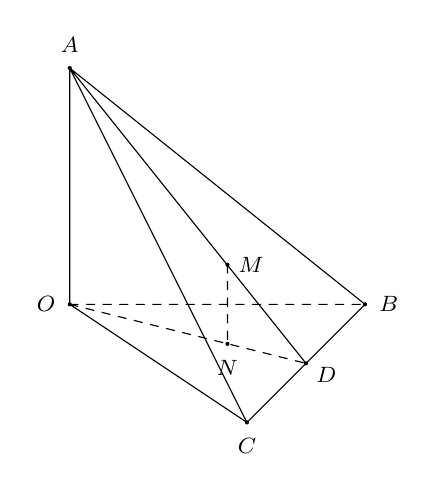
\begin{tikzpicture}[scale=0.75, font=\footnotesize, line join=round, line cap=round, >=stealth]
	\path 
	(0,4) coordinate (A)
	(5,0) coordinate (B)
	(3,-2) coordinate (C)
	(4,-1) coordinate (D)
	(2.67,0.67) coordinate (M)
	(2.67,-0.67) coordinate (N)
	(0,0) coordinate (O)
	;
	\draw (A)--(B)--(C)--(O)--cycle (A)--(D) (A)--(C);
	\draw[dashed] (M)--(N) (O)--(D) (O)--(B);
	\foreach \p/\r in {A/90,B/0,C/-90,O/180,M/0,N/-90,D/-30}
	\fill (\p) circle (1pt) node[shift={(\r:3mm)}]{$\p$};
	\end{tikzpicture}
}	
}
\end{vd}
\begin{vd}
	Cho hình chóp $S.ABC$. Các điểm $M,\ N,\ P$ tương ứng là trung điểm của $SA,\ SB,\ SC$. Đường thẳng qua $S$ vuông góc với mặt phẳng $(ABC)$ và cắt mặt phẳng đó tại $H$. Chứng minh rằng $SH\perp (MNP)$.
	\loigiai{
\immini{
Do $\heva{&MN\parallel AB\\& MP\parallel AC}$ nên $(MNP)\parallel (ABC)$.\\
Mặt khác $SH\perp (ABC)$. Do đó $SH\perp (MNP)$.
}{
	\begin{tikzpicture}[scale=0.9, font=\footnotesize, line join=round, line cap=round, >=stealth]
	\def\bc{4} % cạnh BC
	\def\ba{2} % cạnh BA
	\def\as{4} % cạnh AS
	\def\gocB{30} % góc B của đáy
	\coordinate[label=below left:$B$] (B) at (0,0);
	\coordinate[label=above right:$A$] (A) at (\gocB:\ba);
	\coordinate[label=below:$C$] (C) at (\bc,0);
	%\coordinate[label=right:$D$] (D) at ($(C)-(B)+(A)$);
	\coordinate[label=above:$S$] (S) at (75:\as); % chỉnh 75 và as để thay đổi S
	\coordinate[label=above:$M$] (M) at ($(A)!.5!(S)$);
	\coordinate[label=above right:$N$] (N) at ($(B)!.5!(S)$);
	\coordinate[label=right:$P$] (P) at ($(C)!.5!(S)$);
	%\coordinate[label=right:$Q$] (Q) at ($(D)!.5!(S)$);
	%\coordinate[label=below:$O$] (O) at ($(A)!.5!(C)$);
	\draw (N)--(P);
	\draw[dashed] (P)--(M)--(N);
	\draw (B)--(C)--(S)--cycle (S)--(C);
	\draw[dashed] (A)--(C) (S)--(A)--(B);
	\foreach \diem in {A,B,C,S,M,N,P}	\fill (\diem)circle(1.5pt);
	\end{tikzpicture}
}
}
\end{vd}
\begin{vd}%[1H3B3-2]
	Cho tứ diện $ABCD$ có $ABD$ và $DBC$ là những tam giác cân tại $A$ và $D$. Gọi $I$ là trung điểm của $BC$ và $AH$ là đường cao của tam giác $ADI$.
	\begin{enumEX}{2}
	\item Chứng minh $BC \perp AD$.
	\item Chứng minh $AH \perp (BCD)$.
	\end{enumEX}
	\loigiai{
	\begin{enumEX}{1}
	\item Chứng minh $BC \perp AD$.\\
	$AI$ là trung tuyến $\triangle ACB$ cân tại $A \Rightarrow AI \perp BC$.\\
	$DI$ là trung tuyến $\triangle DCB$ cân tại $D \Rightarrow DI \perp BC$.
	\immini{
	Ta có $ \heva{& BC\perp AI \quad(\text{cmt})\\ & BC\perp DI \quad(\text{cmt}) \\& AI \cap DI=I \\ & AI, DI \subset (ADI). } $
	$\\ \Rightarrow BC \perp (ADI) $.\\
	Mà $AD \subset (ADI) \Rightarrow BC \perp AD$.
	\item Chứng minh $AH \perp (BCD)$.\\
	Ta có $ \heva{& AH\perp DI \quad(\text{giả thiết} )\\ & AH \perp BC \quad(\text{do}\, BC \perp (ADI), AH \subset (ADI)) \\& DI\cap BC=I \\ & DI, BC \subset (BCD). } $\\
	$ \Rightarrow AH\perp (BCD) $.
		}
{
\begin{tikzpicture}[scale=1, font=\footnotesize, line join=round, line cap=round, >=stealth]
	\def\ac{4} % cạnh AC
	\def\ab{3} % cạnh AB
	\def\as{3} % cạnh AS
	\def\gocA{35} % góc A của đáy
	\coordinate[label=left:$D$] (D) at (0,0);
	\coordinate[label=right:$B$] (B) at (\ac,0);
	\coordinate[label=below left:$C$] (C) at (-\gocA:\ab);
	\coordinate[label=above:$A$] (A) at (70:\as);
	\coordinate[label=below right:$I$] (I) at ($(C)!0.5!(B)$);
	\coordinate (A') at ($(A)+(0,-\as-1)$);
	\draw[opacity=0,name path=a](A)--(A');
	\draw[opacity=0,name path=b](D)--(I);
	\path[name intersections={of= a and b}] coordinate (H)at(intersection-1);
	\fill (H)circle(1.5pt)node[below]{$H$};
	\draw (D)--(C)--(B)--(A)--cycle (A)--(C);
	\draw[dashed] (D)--(I) (A)--(H);
	\draw[line width=0.4pt,black,dashed] (D)--(B)node[scale=1,pos=0.6,black,sloped]{$|$};
	\draw[line width=0.4pt,black] (D)--(C)node[scale=1,pos=0.6,black,sloped]{$|$};
	\foreach \diem in {A,B,C,D,I}\fill (\diem)circle(1.5pt);
\end{tikzpicture}
}
	\end{enumEX}
	}
\end{vd}
\begin{vd}%[1H3B3-2]
	Cho hình chóp $ S.ABCD $ có đáy $ ABCD $ là hình vuông tâm $ O $ và $ SA \perp (ABCD) $. Gọi $ H $, $ K $ lần lượt là hình chiếu của $ A $ trên $ SB $ và $ SD $.
	\begin{enumEX}{2}
	\item Chứng minh $ BC \perp SB $ và $ CD \perp SD $.
	\item Chứng minh $ BD \perp (SAC) $.
	\item Chứng minh $ HK \perp (SAC) $.
	\item Chứng minh $ AH \perp (SBC) $.
	\item Chứng minh $ AK \perp (SCD) $.
	\item Gọi $ I $ là hình chiếu của $ A $ lên $ SC $. Chứng minh $ AH $, $ AI $, $ AK $ đồng phẳng.
	\end{enumEX}
	\loigiai{
	\begin{enumEX}{1}
	\item Chứng minh $ BC \perp SB $ và $ CD \perp SD $.
	\immini{
	Ta có $ \heva{& BC\perp AB \quad(\text{do}\, ABCD\, \text{là hình vuông})\\ & BC \perp SA \quad(\text{do}\, SA \perp (ABCD), BC \subset (ABCD)) \\& AB \cap SA=A \\ & AB, SA \subset (SAB). } $\\
	$ \Rightarrow BC \perp (SAB) $.\\
	Mà $ SB \subset (SAB) \Rightarrow BC \perp SB$.\\
	Tương tự $ \heva{& CD\perp AD \quad(\text{do}\, ABCD)\, \text{là hình vuông}\\ & CD \perp SA \quad(\text{do}\, SA \perp (ABCD), CD \subset (ABCD)) \\& AD \cap SA=A \\ & AD, SA \subset (SAD). } $\\
	$ \Rightarrow CD \perp (SAD) $.\\
	Mà $ SD \subset (SAD) \Rightarrow CD \perp SD$.
	}
	{
	\begin{tikzpicture}[scale=1, font=\footnotesize, line join=round, line cap=round, >=stealth]
	\def\bc{4} % cạnh BC
	\def\ba{2} % cạnh BA
	\def\h{4} % đường cao
	\def\gocB{30} % góc B của đáy
	\coordinate[label=below left:$B$] (B) at (0,0);
	\coordinate[label=below:$A$] (A) at (\gocB:\ba);
	\coordinate[label=below:$C$] (C) at (\bc,0);
	\coordinate[label=right:$D$] (D) at ($(C)-(B)+(A)$);
	\coordinate[label=above:$S$] (S) at ($(A)+(90:\h)$);
	\coordinate[label=above:$O$] (O) at ($(A)!0.5!(C)$);
	\coordinate[label=left:$H$] (H) at ($(S)!0.6!(B)$);
	\coordinate[label=right:$K$] (K) at ($(S)!0.6!(D)$);
	\coordinate[label=right:$I$] (I) at ($(S)!0.3!(C)$);
	\draw (B)--(C)--(D)--(S)--cycle (S)--(C);
	\draw[dashed] (A)--(D) (S)--(A)--(B) (A)--(C) (B)--(D) (A)--(H)--(K)--cycle (A)--(I);
	\foreach \diem in {A,B,C,D,S,O,H,K,I}	\fill (\diem)circle(1.5pt);
	\pic [draw=black,angle radius=2.5mm] {right angle = S--A--D};
	\pic [draw=black,angle radius=2.5mm] {right angle = A--H--B};
	\pic [draw=black,angle radius=2.5mm] {right angle = A--K--D};
	\pic [draw=black,angle radius=2.5mm] {right angle = A--I--C};
	\pic [draw=black,angle radius=2.5mm] {right angle = A--O--B};
	\pic [draw=black,angle radius=3mm] {right angle = A--B--C};
	\end{tikzpicture}
	}
	\item Chứng minh $ BD \perp (SAC) $.\\
	Ta có $ \heva{& BD\perp AC \quad(\text{do}\, AC, BD \, \text{là hai đường chéo hình vuông})\\ & BD \perp SA \quad(\text{do}\, SA \perp (ABCD), BD \subset (ABCD)) \\& SA \cap AC=A \\ & SA, AC \subset (SAC). } $\\
	$ \Rightarrow BD \perp (SAC) $.
	\item Chứng minh $ HK \perp (SAC) $.\\
	Xét $ \triangle SAB $ vuông tại $ A $, đường cao $ AH $, ta có $ SH \cdot SB =SA^2$.\qquad $ (1) $\\
	Xét $ \triangle SAD $ vuông tại $ A $, đường cao $ AK $, ta có $ SK \cdot SD =SA^2$.\qquad $ (2) $\\
	Từ $ (1) $ và $ (2) $ suy ra $ SH=SK \Rightarrow \dfrac{SH}{SB}=\dfrac{SK}{SD}\Rightarrow HK \parallel BD$.\\
	Mặt khác, $ BD \perp (SAC) $ nên $ HK \perp (SAC) $.
	\item Chứng minh $ AH \perp (SBC) $.\\
	Ta có $ \heva{& AH\perp SB \quad(H\text{ là hình chiếu của $ A $ lên $ SB $})\\ & AH \perp BC \quad(\text{do}\, BC \perp (SAB), AH \subset (SAB)) \\& SB \cap BC=B \\ & SB, BC \subset (SBC). } $\\
	$ \Rightarrow AH \perp (SBC) $.
	\item Chứng minh $ AK \perp (SCD) $.\\
	Ta có $ \heva{& AK\perp SD \quad(K\text{ là hình chiếu của $ A $ lên $ SD $})\\ & AK \perp CD \quad(\text{do}\, CD \perp (SAD), AK \subset (SAD)) \\& SD \cap CD=D \\ & SD, CD \subset (SCD). } $\\
	$ \Rightarrow AK \perp (SCD) $.
	\item Gọi $ I $ là hình chiếu của $ A $ lên $ SC $. Chứng minh $ AH $, $ AI $, $ AK $ đồng phẳng.\\
	Ta có $\heva{& AH \perp (SBC) \Rightarrow AH \perp SC \\ & AK \perp (SCD) \Rightarrow AK \perp SC.} $\\
	Mặt khác do $ AI \perp SC$ nên $ AH $, $ AI $, $ AK $ đồng phẳng. 
	\end{enumEX}
	}
\end{vd}
\subsubsection{Bài tập áp dụng}
\begin{bt}
	Cho hình chóp $S.ABCD$ có đáy $ABCD$ là hình thoi, $SA\perp (ABCD)$. Chứng minh rằng $BD\perp(SAC)$.
	\loigiai{
		\immini{Ta có $SA \perp (ABCD)\Rightarrow SA\perp BD$.\hfill $(1)$\\
			Lại có $BD\perp AC$ (vì $ABCD$ là hình thoi).\hfill $(2)$\\
			$AC,SA\subset (SAC)$, $AC$ cắt $SA$ tại $A$.\hfill$(3)$\\
			Từ $(1)$, $(2)$, $(3)$ ta suy ta $BD\perp (SAC)$.}{\begin{tikzpicture}[scale=0.7, line join=round, line cap=round]
				\tkzDefPoints{0/0/A,-1.3/-1.6/B,2.5/-1.6/C}
				\coordinate (D) at ($(A)+(C)-(B)$);
				\coordinate (S) at ($(A)+(0,3)$);
				\coordinate (O) at ($(A)!0.5!(C)$);
				\tkzDrawPolygon(S,B,C,D)
				\tkzDrawSegments(S,C)
				\tkzMarkRightAngles[size=0.3](S,A,C B,O,C)
				\tkzDrawSegments[dashed](A,S A,B A,D B,D A,C)
				\tkzDrawPoints[fill=black,size=1.5pt](D,C,A,B,S)
				\tkzLabelPoints[above](S)
				\tkzLabelPoints[below](A,B,C)
				\tkzLabelPoints[right](D)
		\end{tikzpicture}}
	}
\end{bt}
\begin{bt}%[1C8B2-2]
	Cho hình chóp $S.ABCD$ có $SA\perp (ABCD)$, đáy $ABCD$ là hình bình hành có $AC$ cắt $BD$ tại $O$. Gọi $M$ là trung điểm của $SC$. Chứng minh rằng $OM\perp (ABCD)$.
	\loigiai{
	\immini{Vì $ABCD$ là hình bình hành nên $OA=OC$. Ta có $OM$ là đường trung bình của tam giác $SAC$ nên $OM\parallel SA$. Mà $SA\perp (ABCD)$ nên $OM\perp (ABCD)$.}{\begin{tikzpicture}[scale=0.7, line join=round, line cap=round]
	\tkzDefPoints{0/0/A,-1.3/-1.6/B,2.5/-1.6/C}
	\coordinate (D) at ($(A)+(C)-(B)$);
	\coordinate (S) at ($(A)+(0,3)$);
	\tkzDrawPolygon(S,B,C,D)
	\tkzDrawSegments(S,C)
	\tkzDrawSegments[dashed](A,S A,B A,D)
	\tkzInterLL(A,C)(B,D)\tkzGetPoint{O}	
	\coordinate (M) at ($(S)!0.5!(C)$);
	\tkzDrawSegments[dashed](A,C B,D M,O)
	\tkzDrawPoints[fill=black,size=1.5pt](D,C,A,B,S,O,M)
	\tkzLabelPoints[above](S)
	\tkzLabelPoints[below](A,B,C,O)
	\tkzLabelPoints[right](D,M)
	\end{tikzpicture}}
	}
\end{bt}
\begin{bt}%[1H3B3-2]
	Cho hình chóp $S.ABCD$ có đáy là hình thoi, tâm $O$. Biết $SA=SC$ và $SB=SD$.
	\begin{listEX}[1]
		\item Chứng minh: $SO \perp(ABCD)$.
		\item Gọi $I$, $K$ lần lượt là trung điểm của $BA$ và $BC$. Chứng minh: $IK \perp SD$.
	\end{listEX}
	\loigiai 
	{\immini
		{
			\begin{listEX}[1]
				\item Ta có 
				$\heva{& SO \perp AC~\left(\text{vì}~\triangle SAC~\text{cân tại}~S\right)\\ & SO \perp BD~\left(\text{vì}~\triangle SBD~\text{cân tại}~S\right)\\ &AC, BD \subset (ABCD)\\& AC\cap BD=O}$\\
				$\Rightarrow SO \perp (ABCD)$.\\ 
				\item
				Ta có $\heva{& AC \perp BD~\left(\text{tính chất hình thoi}\right)\\ & AC \perp SO~\left(\text{vì}~SO \perp (ABCD)\right)\\ &BD, SO \subset (SBD)\\& BD\cap SO=O}$\\
				$\Rightarrow AC \perp (SBD) \Rightarrow AC \perp SD$.\\
				Ta có $IK$ là đường trung bình của $\triangle ABC$ nên $IK \parallel AC$.\\
				Mà $AC \perp SD$ nên $IK \perp SD$.
			\end{listEX}
		}
		{
			\begin{tikzpicture}[line join=round, line cap=round,thick,scale=0.6]
				\def\h{6}
				\path
				(0,0) coordinate (A)
				(-3,-3) coordinate (B)
				(6,0) coordinate (D)
				($(B)+(D)-(A)$) coordinate (C)
				(intersection of A--C and B--D) coordinate (O)
				(barycentric cs:B=1,A=1)coordinate(I)
				(barycentric cs:B=1,C=1)coordinate(K)
				;
				\path ($(0,\h)+(O)$) coordinate (S);
				\draw[dashed] (A)--(D) (A)--(S) (A)--(B) (A)--(C) (B)--(D) (S)--(O) (I)--(K);
				\draw (B)--(C) --(D);
				\draw (S)--(B) (S)--(C) (S)--(D);
				\foreach \i/\j in {A/160,B/-120,C/-45,D/0,O/-90,S/90,I/120,K/-90}\fill (\i) circle(1pt) ($(\i) + (\j:4mm)$)node{$\i$};
				\draw 
				pic[draw, angle radius=2mm]{right angle=A--O--B}
				pic[draw, angle radius=2mm]{right angle=S--O--D};
			\end{tikzpicture}
		}
	}
\end{bt}
\begin{bt}%[1H3B3-2]
	Cho hình chóp $S.ABC$ có tam giác $ABC$ vuông tại $B$ và $SA \perp (ABC)$. Gọi $AH$, $AK$ lần lượt là các đường cao trong tam giác $SAB$ và $SAC$.
	\begin{enumEX}{2}
	\item Chứng minh tam giác $SBC$ vuông.
	\item Chứng minh tam giác $AHK$ vuông.
	\item Chứng minh $SC \perp (AHK)$.
	\item Chứng minh tam giác $SHK$ vuông.
	\item Gọi $I=HK \cap BC$. Chứng minh $IA \perp (SAC)$.
	\end{enumEX}
	\loigiai{
	\begin{enumEX}{1}
	\item Chứng minh tam giác $SBC$ vuông.
	\immini
	{
	Ta có $ \heva{& BC\perp AB \quad(\triangle ABC\,\text{vuông tại } B)\\ & BC \perp SA \quad(\text{do}\, SA \perp (ABC), BC \subset (ABC)) \\& AB \cap SA=A \\ & AB, SA \subset (SAB). } $\\
	$ \Rightarrow BC \perp (SAB) $.\\
	Mà $SB \subset (SAB)$ nên $BC \perp SB$.\\
	Vậy tam giác $SBC$ vuông tại $B$.\\
	\item Chứng minh tam giác $AHK$ vuông.\\
	Ta có $ \heva{& AH\perp SB \quad(\text{giả thiết} )\\ & AH \perp BC \quad(\text{do}\, BC \perp (SAB), AH \subset (SAB)) \\& SB \cap BC=B \\ & SB, BC \subset (SBC). } $\\
	$ \Rightarrow AH \perp (SBC) $.\\
	Mà $HK \subset (SBC)$ nên $AH \perp HK$.\\
	Vậy tam giác $AHK$ vuông tại $H$.
	}
	{
	\begin{tikzpicture}[scale=1, font=\footnotesize, line join=round, line cap=round, >=stealth]
	\def\ac{4} % cạnh AC
	\def\ab{2} % cạnh AB
	\def\h{4} % chiều cao
	\def\gocA{40} % góc A của đáy
	\coordinate[label=left:$A$] (A) at (0,0);
	\coordinate[label=right:$C$] (C) at (\ac,0);
	\coordinate[label=below left:$B$] (B) at (-\gocA:\ab);
	\coordinate[label=above:$S$] (S) at ($(A)+(90:\h)$);
	\coordinate[label=right:$H$] (H) at ($(S)!0.6!(B)$);
	\coordinate[label=right:$K$] (K) at ($(S)!0.33!(C)$);
	\coordinate (H') at ($(K)!3!(H)$);
	\coordinate (B') at ($(C)!2!(B)$);
	\draw[opacity=0,name path=a](K)--(H');
	\draw[opacity=0,name path=b](B)--(B');
	%	\path[name intersections={of= a and b}] coordinate (M)at(intersection-1);
	\path[name intersections={of= a and b}] coordinate (I)at(intersection-1);
	\fill (I)circle(1.5pt)node[below]{$I$};
	\draw (B)--(C)--(S)--(A) (S)--(B) (A)--(H) (K)--(I)--(C) (A)--(I);
	\draw[dashed] (A)--(C) (A)--(K) (A)--(B);
	\foreach \diem in {A,B,C,S,H,K}	\fill (\diem)circle(1.5pt);
	\pic [draw=black,angle radius=2.5mm] {right angle = S--A--C};
	\pic [draw=black,angle radius=2.5mm] {right angle = A--B--C};
	\pic [draw=black,angle radius=2.5mm] {right angle = A--H--B};
	\pic [draw=black,angle radius=2.5mm] {right angle = A--K--C};
	\end{tikzpicture}
	}
	\item Chứng minh $SC \perp (AHK)$.\\
	Ta có $ \heva{& SC\perp AK \quad(\text{giả thiết} )\\ & SC \perp AH \quad(\text{do}\, AH \perp (SBC), SC \subset (SBC)) \\& AK\cap AH=A \\ & AK, AH \subset (AHK). } $\\
	$ \Rightarrow SC \perp (AHK) $.
	\item Chứng minh tam giác $SHK$ vuông.\\
	Ta có $ SC \perp (AHK) $. Mà $HK \subset (AHK) \Rightarrow SC \perp HK$.\\
	Vậy tam giác $SHK$ vuông tại $K$.
	\item Gọi $I=HK \cap BC$. Chứng minh $IA \perp (SAC)$.\\
	Ta có $ \heva{& IA\perp SA \quad(\text{do}\, SA \perp (ABC) )\\ & IA \perp SC \quad(\text{do}\, SC \perp (AHK), IA \subset (AHK)) \\& SA \cap SC=A \\ & SA, SC \subset (SAC). } $\\
	$ \Rightarrow IA \perp (SAC) $.
	\end{enumEX}
	}
\end{bt}
\begin{bt}%[1H3K3-2]
	Cho hình chóp $S.ABC$ có $SA \perp (ABC)$, tam giác $ABC$ vuông cân tại $B$. Gọi $G$ là trọng tâm của tam giác $SAC$ và $N$ là điểm thuộc cạnh $SB$ sao cho $SN=2NB$.
	\begin{enumEX}{2}
	\item Chứng minh $BC \perp (SAB)$.
	\item Chứng minh $NG \perp (SAC)$.
	\end{enumEX}
	\loigiai{
	\begin{enumEX}{1}
	\item Chứng minh $BC \perp (SAB)$.
	\immini{
	Ta có $ \heva{& BC\perp AB \quad( \triangle ABC\,\text{vuông cân tại}\, B)\\ & BC \perp SA \quad(\text{do}\, SA \perp (ABC), BC \subset (ABC)) \\& AB\cap SA=A \\ & AB, SA \subset (SAB). } $\\
	$ \Rightarrow BC\perp (SAB) $.
	\item Chứng minh $NG \perp (SAC)$.\\
	Ta có $ \heva{& BH\perp AC \quad( BH\,\text{là trung tuyến}\, \triangle ABC )\\ & BH \perp SA \quad(\text{do}\, SA \perp (ABC), BH \subset (ABC)) \\& AC\cap SA=A \\ & AC, SA \subset (SAC). } $\\
	$ \Rightarrow BH\perp (SAC) \quad (\ast)$\\
	Ta có $G$ là trọng tâm $\triangle SAC \Rightarrow \dfrac{SG}{GH}=2.$\\
	Lại có $\dfrac{SN}{NB}=2$. \\
	Nên theo Thales đảo trong $\triangle SBH$, ta có $NG \parallel BH$.\\
	Vậy từ $(\ast) \Rightarrow NG \perp (SAC)$.
	}
	{
	\begin{tikzpicture}[scale=0.8, font=\footnotesize, line join=round, line cap=round, >=stealth]
	\def\ac{6} % cạnh AC
	\def\ab{4} % cạnh AB
	\def\h{4} % chiều cao
	\def\gocA{50} % góc A của đáy
	\coordinate[label=left:$A$] (A) at (0,0);
	\coordinate[label=right:$C$] (C) at (\ac,0);
	\coordinate[label=above right:$H$] (H) at ($(C)!0.5!(A)$);
	\coordinate[label=below:$B$] (B) at ($(H)+(0,-2.5)$);
	\coordinate[label=above:$S$] (S) at ($(A)+(90:\h)$);
	\coordinate (M) at ($(S)!0.5!(A)$);
	\coordinate[label=above right:$G$] (G) at (intersection cs:first line={(S)--(H)}, second line={(C)--(M)});
	\coordinate (G') at ($(G)+(B)-(H)$);
	\coordinate[label=below left:$N$] (N) at (intersection cs:first line={(G)--(G')}, second line={(S)--(B)});
	\draw (A)--(B)--(C)--(S)--cycle (S)--(B);
	\draw[dashed] (A)--(C) (B)--(H)--(S) (C)--(M) (G)--(N);
	\foreach \diem in {A,B,C,S,H,M,G,N}	\fill (\diem)circle(1.5pt);
	\pic [draw=black,angle radius=2.5mm] {right angle = S--A--C};
	\pic [draw=black,angle radius=2.5mm] {right angle = A--B--C};
	\end{tikzpicture}
	}
	\end{enumEX}
	}
\end{bt}
\begin{dang}{Một số bài toán liên hệ giữa quan hệ song song và quan hệ vuông góc khác}
\end{dang}
\subsubsection{Ví dụ minh hoạ}
\begin{vd}
	Cho mặt phẳng $(P)$ và ba điểm $A$, $B$, $C$ thỏa mãn $(P)\perp AB$ và $(P)\perp BC$. Chứng minh rằng $(P)\perp AC$.
	\loigiai{
	Vì hai đường thẳng $AB$ và $AC$ cùng đi qua điểm $B$ và vuông góc với mặt phẳng $(P)$ nên hai đường thẳng này trùng nhau. Suy ra $A$, $B$, $C$ là ba điểm thẳng hàng và $(P)\perp AC$.
	}
\end{vd}
\begin{vd}%[1T8B2-2]
	\begin{enumerate}
	\item Cho hình chóp $S.ABCD$ có các cạnh bên bằng nhau, đáy $A B C D$ là hình vuông tâm $O$ (Hình bên trái). Gọi $d$ là đường thẳng đi qua $S$ và vuông góc với mặt phẳng $(ABCD)$. Chứng minh $d$ đi qua $O$.
	\item Cho đoạn thẳng $AB$ có $O$ là trung điểm. Gọi $(P)$ là mặt phẳng đi qua $O$ và vuông góc với $AB$; $M$, $N$ là hai điểm cách đều hai đầu của đoạn thẳng $A B$ sao cho $M$, $N$, $O$ không thẳng hàng (Hình bên phải). Chứng minh $M$ và $N$ thuộc mặt phẳng $(P)$.
	\end{enumerate}
	\begin{multicols}{2}
	\begin{center}
	\begin{tikzpicture}[scale=0.8,font=\footnotesize,line join = round, line cap = round, >= stealth]
	\tkzDefPoints{0/0/A, 4/0/x, -2/-1.5/y, 0/3/z}
	\coordinate (D) at ($(A)+(x)$);
	\coordinate (B) at ($(A)+(y)$);
	\coordinate (C) at ($(B)+(x)$);
	\coordinate (O) at ($(A)!1/2!(C)$);
	\coordinate (S) at ($(O)+(z)$);
	\coordinate (d) at ($(S)!1/2!(O)$);
	\tkzDrawPolygon(S,B,C)
	\draw (S)--(D)--(C);
	\draw[dashed] (S)--(A)--(B)--(D)--(A)--(C) (S)--(O);
	\tkzDrawPoints[fill=black](A,B,C,S,O)
	\tkzLabelPoints[left](A,B,d)
	\tkzLabelPoints[right](D,C)
	\tkzLabelPoints[above](S)
	\tkzLabelPoints[below](O)
	\tkzMarkRightAngle(A,O,B)
	\end{tikzpicture}
	\end{center}
	\begin{center}
	\begin{tikzpicture}[scale=0.6, font=\footnotesize, line join=round, line cap=round, >=stealth]
	\tkzDefPoints{0/0/E, 3/1/F, 0/5/H, 2/4.5/M, 1/2/O, -2/2/A,1/4.5/N}
	\tkzDefPointBy[translation = from E to H](F)
	\tkzGetPoint{G}
	\tkzDefPointBy[symmetry = center O](A)
	\tkzGetPoint{B}
	\tkzInterLL(F,G)(M,B)
	\tkzGetPoint{C}
	\tkzInterLL(F,G)(O,B)
	\tkzGetPoint{D}
	\tkzInterLL(E,H)(M,A)
	\tkzGetPoint{J}
	\tkzInterLL(E,H)(O,A)
	\tkzGetPoint{K}
	\tkzInterLL(E,H)(N,A)
	\tkzGetPoint{J'}
	\tkzLabelPoints[below](A,B,O)
	\tkzLabelPoints[above](M,N)
	\tkzDrawSegments(E,F F,D C,G G,H H,E M,O M,B B,O A,K A,J J',A N,O N,B)
	\tkzDrawSegments[dashed](M,J O,K C,D N,J')
	\end{tikzpicture}
	\end{center}
	\end{multicols}
	\loigiai{
	\begin{enumerate}
	\item Ta có $SA=SC$ suy ra $SO \perp AC$; $SB=SD$ suy ra $SO \perp BD$. Suy ra $SO \perp (ABCD)$.\\
	Theo giả thiết, ta có đường thẳng $d$ đi qua $S$ và vuông góc với $(ABCD)$.\\
	Do qua điểm $S$ chỉ có duy nhất một đường thẳng vuông góc với $(ABCD)$ nên $d$ phải trùng với đường thẳng $SO$, suy ra $d$ đi qua $O$.
	\item Ta có $MA=MB$ suy ra $OM \perp AB$; $NA=NB$ suy ra $ON \perp AB$. Suy ra $AB \perp (OMN)$.\\
	Theo giả thiết, ta có $(P)$ là mặt phẳng đi qua $O$ và vuông góc với $AB$.\\
	Do qua điểm $O$ chỉ có duy nhất một mặt phẳng vuông góc với $AB$ nên $(P)$ phải trùng với $(OMN)$, suy ra $M$ và $N$ thuộc $(P)$.
	\end{enumerate}
	}
\end{vd}
\begin{vd}%[1T8B2-2]
	\immini{
	Cho hình hộp $ABCD.A'B'C'D'$ có $AA' \perp (ABCD)$. Gọi $M$ và $N$ lần lượt là trung điểm của $AB$ và $BC$.
	\begin{enumerate}
	\item Qua $M$ vẽ đường thẳng $a$ song song với $AA'$. Chứng minh $a \perp (ABCD)$.
	\item Qua $N$ vẽ đường thẳng $b$ vuông góc với $(ABCD)$.
	Chứng minh $b \parallel AA'$.
	\end{enumerate}
	}
	{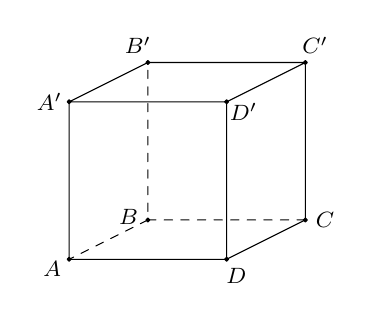
\begin{tikzpicture}[scale=.5, font=\footnotesize, line join=round, line cap=round, >=stealth]
	\path
	(0,0) coordinate (A)
	(2,1) coordinate (B)
	(6,1) coordinate (C)
	(4,0) coordinate (D)
	(0,4) coordinate (A')
	(2,5) coordinate (B')
	(6,5) coordinate (C')
	(4,4) coordinate (D')
	(5,1.5) coordinate (H)
	;
	\draw (A)--(A')--(B')--(C')--(D')--(A') (D)--(A) (D)--(C) (D)--(D') (C)--(C');
	\draw[dashed] (C)--(B)--(B') (B)--(A);
	\foreach \x/\g in {A/-150, B/170, C/0, D/-60, A'/180,B'/120,C'/60,D'/-30}
	\draw[fill=black] (\x) circle (.05)+(\g:.5) node{$\x$};
	\end{tikzpicture}}
	\loigiai{
	\begin{enumerate}
	\item Theo đề bài ta có $a \parallel AA'$ và $AA' \perp (ABCD)$, suy ra $a \perp (ABCD)$.
	\item Theo đề bài ta có $b \perp (ABCD)$ và $AA' \perp (ABCD)$, suy ra $b \parallel AA'$.
	\end{enumerate}
	}
\end{vd}
\begin{vd}
	Cho mặt phẳng $(P)$ và đường thẳng $a$ cắt $(P)$ tại $O$ sao cho $a\perp(P)$. Giả sử $b$ là đường thẳng đi qua điểm $O$ và $b\perp a$. Chứng minh rằng $b\subset (P)$.
	\loigiai{
		Ta lấy điểm $M$ trong mặt phẳng $(P)$, $M$ khác $O$. Nếu $M\in b$ thì $b\subset(P)$. Xét $M\notin b$. Gọi $c$ là đường thẳng đi qua $O$, $M$ và $(Q)$ là mặt phẳng đi qua $b$, $c$. Do $a\perp b$, $a\perp c$ nên $a\perp (Q)$. Qua điểm $O$ có hai mặt phẳng $(P)$ và $(Q)$ cùng vuông góc với đường thẳng $a$, suy ra hai mặt phẳng đó trùng nhau theo Tính chất 1. Vậy $b\subset (P)$.
	}
\end{vd}
\begin{vd}%[1T8B2-2]
	\immini{
	Cho ba đoạn thẳng $OA$, $OB$, $OC$ đôi một vuông góc với nhau.
	\begin{enumerate}
	\item Cho $M$ là trung điểm của $CA$ và $a$ là đường thẳng tùy ý đi qua $M$ và song song với mặt phẳng $(OAB)$. Chứng minh $a \perp OC$.
	\item Gọi $b$ là một đường thẳng tuỳ ý đi qua $C$ và $b$ vuông góc với $OC$. Chứng minh $b \parallel (OAB)$.
	\end{enumerate}
	}
	{
	\begin{tikzpicture}[scale=0.6, font=\footnotesize, line join=round, line cap=round, >=stealth]
	\coordinate (O) at (-2,0);
	\coordinate (A) at (-5,-3);
	\coordinate (B) at (2,0);
	\coordinate (C) at ($(O)+(0,4)$);
	\coordinate (M) at ($(A)!0.5!(C)$);
	\coordinate (H) at (0,3.5);
	\coordinate[label=above:$b$] (H') at ($(C)!-1!(H)$);
	\draw (C)--(A) (C)--(B) (A)--(B);
	\coordinate (K) at ($(B)+(M)-(O)$);
	\coordinate [label=above:$a$](K') at ($(M)!-0.6!(K)$);
	\draw(K)--(M) (H)--(H') (K)--(K');
	\draw[dashed,thin](O)--(B) (C)--(O) (O)--(A);
	\pic[draw,thin,angle radius=2mm] {right angle = C--O--A} pic[draw,thin,angle radius=2mm] {right angle = C--O--B};
	\foreach \i/\g in {C/90,O/-90,A/-90,B/0,M/130}{\draw[fill=black](\i) circle (1.5pt) ($(\i)+(\g:3mm)$) node[scale=1]{$\i$};}
	\end{tikzpicture}
	}
	\loigiai{
	\begin{enumerate}
	\item Ta có $OC \perp OA$ và $OC \perp OB$, suy ra $OC \perp (OAB) \quad (1)$.\\
	Ta có $a \parallel (OAB) \quad (2)$.\\
	Từ $(1)$ và $(2)$ suy ra $a \perp OC$.
	\item Ta có $b \perp OC \quad (3)$.\\
	Từ $(1)$ và $(3)$, suy ra $b \parallel (OAB)$.
	\end{enumerate}
	}
\end{vd}

\subsubsection{Bài tập áp dụng}
\begin{bt}
	Giả sử $ABCD$ và $ABMN$ là hai hình chữ nhật không cùng nằm trong một mặt phẳng. Chứng minh rằng $(ADN)\parallel (BCM)$.
	\loigiai{
	\immini{
	Vì hai đường thẳng $AD$, $AN$ cắt nhau trong mặt phẳng $(ADN)$, $AB\perp AD$, $AB\perp AN$ nên $AB\perp (ADN)$. Do hai đường thẳng $BC$, $BM$ cắt nhau trong mặt phẳng $(BCM)$, $AB\perp BC$, $AB\perp BM$ nên $AB\perp (BCM)$.\\
	Vì hai mặt phẳng $(ADN)$ và $(BCM)$ cùng vuông góc với $AB$ nên $(ADN)\parallel (BCM)$.}{
	\begin{tikzpicture}[line cap=round,line join=round,font=\footnotesize,>=stealth,scale=0.65]
	\coordinate[label=left:$A$] (A) at (0,0);
	\coordinate[label=right:$B$] (B) at (4,0);
	\coordinate[label=below:$D$] (D) at (1.5,-1.5);
	\coordinate[label=below:$C$] (C) at ($(B)+(D)-(A)$);
	\coordinate[label=above:$N$] (N) at	($(A)+(1,3)$);
	\coordinate[label=above:$M$] (M) at	($(B)+(1,3)$);
	\draw (A)--(D)--(N)--cycle (D)--(C)--(M)--(N)--cycle;
	\draw[dashed] (B)--(A) (B)--(C) (B)--(M);
	\foreach \x in {A,B,C,D,M,N} \draw[fill=red] (\x) circle (1pt);
	\end{tikzpicture}}	}
\end{bt}
\begin{bt}%[1C8B2-2]
	\immini{Cho hình hộp $ABCD.A'B'C'D'$ có $AA'\perp (ABCD)$. Chứng minh rằng $AA'\perp (A'B'C'D')$.}{\begin{tikzpicture}[line cap=round,line join=round,font=\footnotesize,>=stealth,scale=.7]
	\coordinate[label=left:$A$] (A) at (0,0);
	\coordinate[label=below:$B$] (B) at (-1.5,-1.5);
	\coordinate[label=right:$D$] (D) at (4,0);
	\coordinate[label=below:$C$] (C) at ($(B)+(D)-(A)$);
	\coordinate[label=left:$A'$] (A') at	($(A)+(0,3)$);
	\coordinate[label=left:$B'$] (B') at ($(B)+(A')-(A)$);
	\coordinate[label=above:$C'$] (D') at ($(D)+(A')-(A)$);
	\coordinate[label=above:$D'$] (C') at ($(B')+(D')-(A')$);
	\draw (A')--(B')--(C')--(D')--cycle (B)--(C)--(D) (B')--(C')--(C) (D)--(D') (B')--(B);
	\draw[dashed] (B)--(A)--(D) (A)--(A');
	\end{tikzpicture}}
	\loigiai{
	Ta có $AA'\perp (ABCD)$ và $(A'B'C'D')\parallel (ABCD)$ nên $AA'\perp (A'B'C'D')$.
	}
\end{bt}
\begin{bt}
	Cho hình chóp $S.ABC$ có $SA\perp (ABC)$. Mặt phẳng $(P)$ khác mặt phẳng $(ABC)$, vuông góc với đường thẳng $SA$ và lần lượt cắt các đường thẳng $SB$, $SC$ tại $B'$, $C'$. Chứng minh rằng $B'C'\parallel BC$.
	\loigiai{
	\immini{Ta có hai mặt phẳng $(ABC)$ và $(P)$ cùng vuông góc với $SA$ nên chúng song song với nhau.\\
	Hơn nữa, $BC$ và $B'C'$ lần lượt là giao tuyến của mặt phẳng $(SBC)$ với hai mặt phẳng song song trên nên chúng song song với nhau.}{\begin{tikzpicture}[scale=1,line join=round,line cap=round]
	\tkzDefPoints{0/0/A,1.2/-1.5/B,4/0/C}
	\coordinate (S) at ($(A)+(0,3)$);
	\tkzDrawPolygon(S,A,B,C)
	\coordinate (B') at ($(S)!0.7!(B)$);
	\coordinate (C') at ($(S)!0.7!(C)$);
	\coordinate (A') at ($(S)!0.7!(A)$);
	\tkzDrawSegments(S,B A',B' B',C')
	\tkzDrawSegments[dashed](A,C A',C')
	\tkzDrawPoints[fill=black,size=1.5pt](A,B,C,S,B',C')
	\tkzLabelPoints[above](S)
	\tkzLabelPoints[below](B)
	\tkzLabelPoints[left](A)
	\tkzLabelPoints[right](C)
	\tkzLabelPoints[below right](B')
	\tkzLabelPoints[above right](C')
	\tkzMarkRightAngles[size=0.3](S,A,B S,A,C)
	\end{tikzpicture}}
	}
\end{bt}
\begin{bt}
	Cho mặt phẳng $(P)$ và đường thẳng $a$ cắt nhau tại điểm $O$, $a\perp (P)$. Giả sử điểm $M$ thỏa mãn $OM\perp (P)$. Chứng minh rằng $M\in a$.
	\loigiai{
	Vì hai đường thẳng $a$ và $OM$ cùng đi qua $O$ và vuông góc với mặt phẳng $(P)$ nên hai đường thẳng này trùng nhau. Suy ra $M\in a$.}
\end{bt}
\begin{bt}
	Cho đường thẳng $d$ và mặt phẳng $(P)$ cắt nhau tại $O$. Lấy các điểm $A$, $B$ thuộc $d$ và khác $O$; các điểm $A'$, $B'$ thuộc $(P)$ thỏa mãn $AA'\perp (P)$, $BB'\perp (P)$. Chứng minh rằng $\dfrac{AA'}{BB'}=\dfrac{OA}{OB}$.
	\loigiai{
	Ta có $\heva{&AA'\perp (P)\\&BB'\perp (P)}\Rightarrow AA'\parallel BB'$.\\
	Xét tam giác $OAA'$ có $BB'\parallel AA'$ nên theo định lí Talet ta có $\dfrac{OA}{OB}=\dfrac{AA'}{BB'}$.
	}
\end{bt}
%=================
\begin{dang}{Phép chiếu vuông góc}
\end{dang}
\subsubsection{Ví dụ minh hoạ}
\begin{vd}
	Cho hình chóp $S . ABC$ có $SA=SB=SC$. Gọi $O$ là hình chiếu của $S$ trên mặt phẳng $(ABC)$.
	\begin{listEX}[1]
		\item Chứng minh rằng $O$ là tâm đường tròn ngoại tiếp tam giác $ABC$.
		\item Xác định hình chiếu của đường thẳng $SA$ trên mặt phẳng $(ABC)$.
		\item Chứng minh rằng nếu $AO \perp BC$ thì $SA \perp BC$.
		\item Xác định hình chiếu của các tam giác $SBC$, $SCA$, $SAB$ trên mặt phẳng $(ABC)$.
	\end{listEX}	
	\loigiai{
		\begin{listEX}[1]
			\item Chứng minh rằng $O$ là tâm đường tròn ngoại tiếp tam giác $ABC$.\\
			Tam giác $SOA$, $SOB$, $SOC$ bằng nhau (c-g-c). Suy ra $OA=OB=OC$. Do đó $O$ là tâm đường tròn ngoại tiếp tam giác $ABC$
			\item Xác định hình chiếu của đường thẳng $SA$ trên mặt phẳng $(ABC)$.
			\immini{
			Vì $O$ là hình chiếu của $S$ lên mặt phẳng $(ABC)$ nên $AO$ là hình chiếu của $SA$ lên mặt phẳng $(ABC)$
			\item Chứng minh rằng nếu $AO \perp BC$ thì $SA \perp BC$.\\
			Ta có $AO \perp BC$, $SO \perp BC$. Suy ra $BC\perp (SAO)\Rightarrow SA \perp BC$. 
			\item Xác định hình chiếu của các tam giác $SBC$, $SCA$, $SAB$ trên mặt phẳng $(ABC)$.\\
			Hình chiếu của tam giác $SBC$ trên mặt phẳng $(ABC)$ là tam giác $OBC$.\\
			Hình chiếu của tam giác $SAB$ trên mặt phẳng $(ABC)$ là tam giác $OAB$.\\
			Hình chiếu của tam giác $SAC$ trên mặt phẳng $(ABC)$ là tam giác $OAC$. }{%
			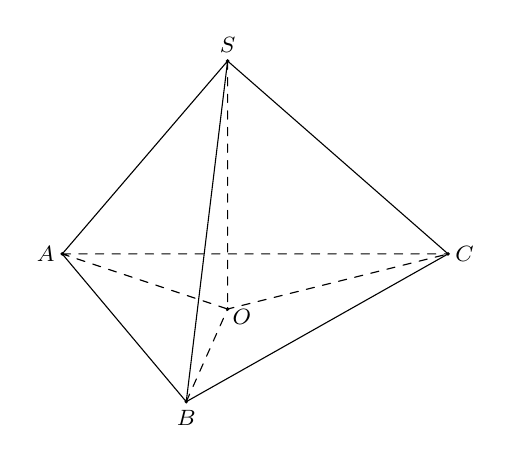
\begin{tikzpicture}[scale=.7,font=\footnotesize,line join=round,line cap=round,>=stealth]
				\path 
				(0,0)coordinate(A) 
				(7,0)coordinate(C) 
				(-50:3.5)coordinate(B) 
				(3,3.5)coordinate(S) 
				(3,-1)coordinate(O) 
				;
				\draw (S)--(A)--(B)--(C)--cycle (B)--(S) 
				;	
				\draw[dashed] (A)--(C) (S)--(O)--(A) (B)--(O)--(C);	
				\foreach \x/\g in {A/180,B/-90,C/0,S/90,O/-30}\fill[black] (\x) circle (1pt) +(\g:.3)node{$\x$};
			\end{tikzpicture}
		}
		\end{listEX}	
	}
\end{vd}
\subsubsection{Bài tập áp dụng}
\begin{bt}%%[1K8B2-5]
	Cho hình chóp $S.ABC$ có $SA \perp(ABC)$, tam giác $ABC$ vuông tại $B$.
	\begin{enumerate}
		\item Xác định hình chiếu của điềm $S$ trên mặt phẳng $(ABC)$.
		\item Xác định hình chiếu của tam giác $SBC$ trên mặt phẳng $(ABC)$.
		\item Xác định hình chiếu của tam giác $SBC$ trên mặt phẳng $(SAB)$.
	\end{enumerate}	
	\loigiai{
		\immini{
			\begin{enumerate}
				\item Do $SA \perp(ABC)$. Suy ra $A$ là hình chiếu của điểm $S$ lên mặt phẳng $(ABC)$.
				\item Hình chiếu của tam giác $SBC$ lên mặt phẳng $(ABC)$ là tam giác $ABC$.
				\item Ta có $BC\perp (SAB)$ nên $B$ là hình chiếu của điểm $C$ lên mặt phẳng $(SAB)$. Do đó hình chiếu của tam giác $SBC$ lên mặt phẳng $(SAB)$ là tam giác $SAB$.
			\end{enumerate}
		}{
			\begin{tikzpicture}[scale=0.7,>=stealth, font=\footnotesize, line join=round, line cap=round]
				\path 
				(0,0)coordinate(A) 
				(5,0)coordinate(C) 
				(-60:3)coordinate(B) 
				($(A)+(0,4)$) coordinate(S) 
				;
				\draw (S)--(A)--(B)--(C)--cycle (B)--(S) 
				pic[draw,angle radius=3mm]{right angle=S--A--B}
				pic[draw,angle radius=3mm]{right angle=S--A--C}
				pic[draw,angle radius=3mm]{right angle=A--B--C}
				;
				\draw [dashed](C)--(A) 
				;	
				\foreach \x/\g in {S/90,A/180,C/0,B/-90}\fill[black] (\x) circle (1pt) +(\g:.3)node{$\x$};
			\end{tikzpicture}
		}	
	}
\end{bt}
\begin{bt}
	\immini{Trên một sân phẳng nằm ngang, tại các điểm $A$, $B$, $C$, $D$ người ta dựng các cột thẳng đứng $AM$, $BN$, $CP$, $DQ$ và nối các sợi dây thẳng giữa $M$ và $P$, $N$ và $Q$ như hình bên.
		\begin{enumerate}
			\item Hãy chỉ ra hình chiếu của các dây $MP$ và $NQ$ trên sân.
			\item Chứng minh rằng nếu $BD\perp AC$ thì $BD\perp MP$.
			\item Chứng minh rằng nếu $ABCD$ là một hình bình hành thì các trung điểm $E$, $F$ tương ứng của các đoạn thằng $MP$ và $NQ$ có cùng hình chiếu trên sân.
	\end{enumerate}}{
		\begin{tikzpicture}[scale=1, font=\footnotesize, line join=round, line cap=round, >=stealth]
			\path 
			(0,0) coordinate (X)
			(5,0) coordinate (Y)
			(1,2.5) coordinate (Z)
			($(Y)-(X)+(Z)$) coordinate (T)
			(3, 1.2) coordinate (O)
			(1.5, 0.5) coordinate (A)
			(4, 0.5) coordinate (D)
			($(A)!2!(O)$) coordinate (C)
			($(D)!2!(O)$) coordinate (B)
			($(A)+(0,3.7)$) coordinate (M)
			($(C)+(0,2.5)$) coordinate (P)
			($(B)+(0,1)$) coordinate (N)
			($(D)+(0,2.5)$) coordinate (Q)
			($(M)!0.5!(P)$) coordinate (E)
			($(N)!0.5!(Q)$) coordinate (F);
			\fill[gray!50] (X)--(Y)--(T)--(Z)--cycle;
			\draw [red, line width =1.5pt] (A)--(M) (C)--(P) (D)--(Q) (B)--(N);
			\draw[line width =1pt] (A)--(C) (B)--(D);
			\draw[red!50!white, line width =1.5pt] (N)--(Q);
			\draw[green!80!black, line width =1.5pt] (M)--(P);
			\foreach \i/\j in {A/-145, D/-45, O/-90, B/180, C/0, M/135, P/30, E/90, N/135, F/90, Q/30}\draw (\i) circle (1pt) ++ (\j:0.3) node {$\i$};
	\end{tikzpicture}}
	\loigiai{
		\begin{enumerate}
			\item Do các cột có phương thẳng đứng và sân thuộc mặt phẳng nằm ngang nên các cột vuông góc với sân. Vậy $A$, $B$, $C$, $D$ tương ứng là hình chiếu của $M$, $N$, $P$, $Q$ trên sân. Do đó $AC$, $BD$ tương ứng là hình chiếu của $MP$, $NQ$ trên sân.
			\item Nếu $BD\perp AC$, mà $AC$ là hình chiếu của $MP$ trên sân và $BD$ thuộc sân nên theo định lý ba đường vuông góc ta có $BD\perp MP$.
			\item Nếu $ABCD$ là một hình bình hành thì các đoạn thẳng $AC$, $BD$ có chung trung điểm $O$. Do $EO$ là đường trung bình của hình thang $ACPM$ nên $EO\parallel MA$. Mặt khác, $MA$ vuông góc với sân nên $EO$ cũng vuông góc với sân. Vậy $O$ là hình chiếu của $E$ trên sân. Tương tự, $O$ cũng là hình chiếu của $F$ trên sân. Vậy $E$ và $F$ có cùng hình chiếu trên sân.
		\end{enumerate}
	}
\end{bt}
\begin{dang}{Góc giữa đường thẳng và mặt phẳng}
	Cho đường thẳng $d$ và mặt phẳng $(P)$ cắt nhau.\\
	Nếu $d\perp (P)$ thì $(d,(P))=90^{\circ}$.
	\begin{center}
	\begin{tikzpicture}[scale=0.6]
	\tkzInit[ymin=-5,ymax=0.5,xmin=-4.1,xmax=4.1]
	\tkzClip %cắt bớt phần ko gian dư
	\tkzDefPoints{-4/-4/M, -2/-1.5/Q, 2/-4/N, -0.5/-3/H}
	\tkzDefPointBy[translation = from M to N](Q) \tkzGetPoint{P}%phép tịnh tiến biến Q thành P
	\tkzDefLine[perpendicular=through H,K=0.4](Q,P) \tkzGetPoint{h}%đường qua H vuông góc QP
	\tkzInterLL(H,h)(Q,P) \tkzGetPoint{h_1}
	\coordinate[label={above right}:$A$] (A) at ($(h_1)+(0,1)$);
	\tkzDefLine[parallel=through H](Q,P) \tkzGetPoint{x}%đường qua H song song MQ
	\coordinate[label={above right}:$O$] (O) at ($(H)!0.4!(x)$);
	\tkzInterLL(A,O)(N,P) \tkzGetPoint{O_1}
	\tkzInterLL(A,O)(P,Q) \tkzGetPoint{O_3}
	\coordinate (O_2) at ($(O)!3.3!(O_1)$);
	\tkzLabelPoints[below](H)
	\tkzDrawLines[add=0 and 0.3](O,H O,A)
	\tkzDrawSegments[dashed](h_1,O_3 O,O_1)
	\tkzDrawSegments(M,N N,P P,O_3 h_1,Q Q,M A,H O_1,O_2)
	\tkzLabelLine[below left,pos=1.3](O,A){$d$}
	\tkzLabelLine[above,pos=1.3](O,H){$d'$}
	\tkzMarkRightAngle(A,H,O)
	\tkzMarkAngles[arc=l,size=0.7cm](A,O,H)
	\tkzLabelAngle[pos=0.9](A,O,H){$\varphi$}
	\tkzMarkAngles[arc=l,size=1.1cm](N,M,Q)
	\tkzLabelAngle[pos=0.7](N,M,Q){$\alpha$}
	\end{tikzpicture}
	\end{center}
	Nếu $d\not\perp (P)$ thì để xác định góc giữa $d$ và $(P)$, ta thường làm như sau
	\begin{enumerate}
	\item Xác định giao điểm $O$ của $d$ và $(P)$.
	\item Lấy một điểm $A$ trên $d$ ($A$ khác $O$). Xác định hình chiếu vuông góc (vuông góc) $H$ của $A$ lên $(P)$. Lúc đó $(d,(P))=(d,d')=\widehat{AOH}$.
	\end{enumerate}
\end{dang}
\subsubsection{Ví dụ minh hoạ}
\begin{vd}%[1C8B3-1]
	Cho hình chóp $S.ABC$ có $SA \perp(ABC)$, $SA=a$, $CA=CB=a \sqrt{7}$, $AB=2a$.
	\begin{listEX}[2]
	\item Gọi $\alpha$ là góc giữa $SB$ và $(ABC)$. Tính $\tan \alpha$.
	\item Tính góc giữa $SC$ và $(SAB)$.
	\end{listEX}
	\loigiai{
	\begin{listEX}[1]
	\item \immini{Do $SA \perp(ABC)$ nên $\alpha=\widehat{SBA}$. Tam giác $SAB$ vuông tại $A$ nên
	$$
	\tan \alpha=\tan \widehat{SBA}=\dfrac{SA}{AB}=\dfrac{a}{2a}=\dfrac{1}{2} .
	$$}{\begin{tikzpicture}[scale=.8,>=stealth, font=\footnotesize, line join=round, line cap=round]
	\path 
	(0,0)coordinate(A) 
	(5,0)coordinate(B) 
	(-60:2.5)coordinate(C) 
	($(A)+(0,3)$) coordinate(S)
	($(A)!0.5!(B)$)coordinate(M)	 
	;
	\draw (S)--(A)--(C)--(B)--cycle (C)--(S) 
	pic[draw,angle radius=3mm]{right angle=S--A--B}
	pic[draw,angle radius=3mm]{right angle=S--A--C}
	pic[draw,angle radius=3mm]{right angle=C--M--B}
	;
	\path
	(S)--(A)node[midway,left]{$a$}
	(M)--(A)node[midway,above]{$a$}
	(B)--(M)node[midway,above]{$a$}
	(C)--(A)node[midway,left]{$a\sqrt{7}$}
	(C)--(B)node[midway,right]{$a\sqrt{7}$}
	;
	\draw [dashed](S)--(M)--(C) (B)--(A) 
	;	
	\foreach \x/\g in {S/90,A/180,C/-90,M/40,B/0}\fill[black] (\x) circle (1pt) +(\g:.3)node{$\x$};
	\end{tikzpicture}}
	\item Gọi $M$ là trung điểm của $A B$. Tam giác $ABC$ cân tại $C$ nên $CM \perp AB$.\\	
	Mặt khác, từ $SA \perp(ABC)$ ta có $CM \perp SA$. Do đó $CM \perp(SAB)$.
	Vậy góc giữa $SC$ và $(SAB)$ bằng $\widehat{CSM}$.\\
	Tam giác $SAC$ vuông tại $A$ nên $SC=\sqrt{S A^2+A C^2}=\sqrt{a^2+7 a^2}=a \sqrt{8}$.\\
	Ta có $AM=\dfrac{1}{2} AB=a$. Do đó, tam giác $SAM$ vuông cân tại $A$ và $SM=a \sqrt{2}$.\\
	Tam giác $CMS$ vuông tại $M$ và $\cos \widehat{CSM}=\dfrac{SM}{SC}=\dfrac{a \sqrt{2}}{a \sqrt{8}}=\dfrac{1}{2}$.\\
	Vậy $\widehat{CSM}=60^{\circ}$ và do đó góc giữa $SC$ và $(SAB)$ bằng $60^{\circ}$.
	\end{listEX}
	}
\end{vd}
\begin{vd}%[1H3B3]
	Cho hình chóp $S.ABCD$ có đáy $ABCD$ là hình vuông cạnh $a$, $SA=a\sqrt{6}$ và $SA$ vuông góc $(ABCD)$. Hãy xác định các góc giữa
	\begin{listEX}[4]
	\item $SC$ và $(ABCD)$.
	\item $SC$ và $(SAB)$.
	\item $SB$ và $(SAC)$.
	\item $AC$ và $(SBC)$.
	\end{listEX}
	\loigiai{
	\begin{center}
	\begin{tikzpicture}[scale=0.8]
	%Hình chóp S.ABCD có SA vuông góc đáy, đáy ABCD là hình chữ nhật.
	\tkzDefPoints{0/0/A, -3/-2/B, 6/0/D}
	\coordinate (C) at ($(B)+(D)-(A)$);
	\coordinate (S) at ($(A)+(0,4.5)$);
	\tkzInterLL(A,C)(B,D) \tkzGetPoint{O}
	% Chú ý MN song song BD.
	\coordinate (M) at ($(S)!0.75!(B)$);
	\coordinate (N) at ($(S)!0.6!(D)$);
	% vẽ đoạn thẳng
	\draw[thick] (S)--(C);
	\draw[thick] (S)--(D);
	\draw[thick] (S)--(B);
	\draw[thick] (B)--(C);
	\draw[thick] (C)--(D) (M)--(C);
	\draw[dashed] (O)--(S)--(A);
	\draw[dashed] (D)--(A);
	\draw[dashed] (A)--(B);
	\draw[dashed] (A)--(C);
	\draw[dashed] (D)--(B);
	%\draw[dashed] (A)--(N);
	\draw[dashed] (A)--(M);
	%\draw[dashed] (M)--(N);
	% Gán nhãn các điểm
	\tkzLabelPoints[below](A)
	\tkzLabelPoints[right](D)
	\tkzLabelPoints[below](B)
	\tkzLabelPoints[below](C)
	\tkzLabelPoints[above](S)
	\tkzLabelPoints[right](O)
	%\tkzLabelPoints[right](N)
	\tkzLabelPoints[left](M)
	% Kí hiệu các góc
	\tkzMarkRightAngle(S,A,D)
	\tkzMarkRightAngle(S,A,B)
	\tkzMarkRightAngle(A,M,S)
	%\tkzMarkRightAngle(A,N,S)
	\tkzMarkRightAngle(A,O,B)
	% Vẽ các điểm
	\tkzDrawPoints(S,A,B,C,D,O,M)
	\tkzMarkAngles[mark=|,arc=l,size=0.7cm](S,C,A)
	\tkzMarkAngles[mark=||,arc=l,size=1.2cm](B,S,C)
	\tkzMarkAngles[mark=|||,arc=l,size=0.5cm](B,S,O)
	\tkzMarkAngles[mark=x,arc=l,size=1.3cm](A,C,M)
	%\tkzLabelAngle[pos=0.9](A,O,H){$\varphi$}
	\end{tikzpicture}
	\end{center}
	\begin{enumerate}
	\item Vì $AC$ là hình chiếu vuông góc của $SC$ lên $(ABCD)$ nên góc giữa $SC$ và $(ABCD)$ là $\widehat{SCA}$.\\
	Trong tam giác $SCA$, ta có $\tan\widehat{SCA}=\dfrac{SA}{SC}=\sqrt{3}$ nên $\left(SC,(ABCD)\right)=\widehat{SCA}=60^{\circ}$.
	\item Vì $BC\perp (SAB)$ tại $B$ nên $SB$ là hình chiếu vuông góc của $SC$ lên $(SAB)$.\\
	Do đó $\left(SC,(SAB)\right)=(SC,SB)=\widehat{CSB}$.\\
	Trong tam giác $SCB$, ta có $\tan\widehat{CSB}=\dfrac{BC}{SB}=\dfrac{a}{a\sqrt{7}}$ nên $\left(SC,(SAB)\right)=\arctan\dfrac{1}{\sqrt{7}}$.
	\item Vì $BO\perp (SAC)$ tại $O$ nên $SO$ là hình chiếu vuông góc của $SB$ lên $(SAC)$.\\ Do đó $\left(SB,(SAC)\right)=(SB,SO)=\widehat{BSO}$.\\
	Trong tam giác $SBO$, ta có $\sin\widehat{BSO}=\dfrac{BO}{SB}=\dfrac{\dfrac{a\sqrt{2}}{2}}{a\sqrt{7}}=\dfrac{1}{\sqrt{14}}$ nên $\left(SB,(SAC)\right)=\arcsin\dfrac{1}{\sqrt{14}}$.
	\item Gọi $M$ là hình chiếu vuông góc của $A$ lên $SB$. Lúc đó $AM\perp SB$ và $AM\perp BC$ (vì $BC\perp(SAB)$ và $AM\subset (SAB)$) nên $AM\perp (SBC)$ tại $M$. Do đó $MC$ là hình chiếu vuông góc của $AC$ lên $(SBC)$.\\ 
	Suy ra $\left(AC,(SBC)\right)=(AC,MC)=\widehat{ACM}$.\\
	Trong tam giác $SAB$, ta có $AM=\dfrac{SA.AB}{SB}=\dfrac{a\sqrt{6}}{\sqrt{7}}$ và trong tam giác $ACM$, ta có $\sin\widehat{ACM}=\dfrac{MA}{AC}=\dfrac{\sqrt{21}}{7}$ nên $\left(AC,(SBC)\right)=\arcsin\dfrac{\sqrt{21}}{7}$.
	\end{enumerate}
	}
\end{vd}
\begin{vd}%[1H3G3]
	Cho hình chóp $S.ABCD$ có đáy là hình vuông cạnh $a$, tâm $O$, $SO$ vuông góc $(ABCD)$. Gọi $M, N$ lần lượt là trung điểm $SA, BC$. Biết rằng góc giữa $MN$ và $(ABCD)$ bằng $60^{\circ}$. Tính góc giữa $MN$ và $(SBD)$.
	\loigiai{
	\begin{center}
	\begin{tikzpicture}
	\tkzDefPoints{0/0/O, -4/-1/A, 1/-1/B, 0/5.5/S}
	\tkzDefPointBy[symmetry = center O](A)
	\tkzGetPoint{C}
	\tkzDefPointBy[symmetry = center O](B)
	\tkzGetPoint{D}
	\tkzDefMidPoint(S,A)
	\tkzGetPoint{M}
	\tkzDefMidPoint(B,C)
	\tkzGetPoint{N}
	\tkzDefMidPoint(A,O)
	\tkzGetPoint{H}
	\tkzDefMidPoint(S,D)
	\tkzGetPoint{K}
	\tkzDrawSegments[dashed](A,D A,C D,C D,B S,D S,O M,N M,H N,H C,K O,K M,K)
	\tkzDrawSegments(A,B B,C S,A S,B S,C)
	\tkzMarkRightAngle[size=.2](B,O,C)
	\tkzMarkRightAngle[size=.2](M,H,N)
	\tkzMarkRightAngle[size=.2](K,O,C)
	\tkzLabelPoints[below](O,A,B,N,H)
	\tkzLabelPoints[above left](S,M,K)
	\tkzLabelPoints[right](C)
	\tkzLabelPoints[left](D)
	\tkzMarkAngles[mark=|,arc=l,size=0.5cm](O,K,C)
	\tkzMarkAngles[arc=l,size=0.7cm](M,N,H)
	%\tkzMarkSegments[mark=||](S,A S,B S,C S,D)
	\end{tikzpicture}
	\end{center}
	Gọi $H$ là trung điểm $AO$. Ta có $MH\parallel SO$ nên $MH\perp (ABCD)$, suy ra $HN$ là hình chiếu vuông góc của $MN$ lên $(ABCD)$. Do đó $\left(MN,(ABCD)\right)=(MN,KN)=\widehat{MNK}=60^{\circ}$.\\
	Trong tam giác $HCN$, ta có $HN^2=HC^2+CN^2-2HC.CN.\cos\widehat{HCN}$, suy ra $HN=\dfrac{a\sqrt{10}}{4}$.\\
	Mà trong tam giác $MNH$, ta có $\sqrt{3}=\tan\widehat{MNH}=\dfrac{MH}{HN}$ nên $MH=\dfrac{a\sqrt{30}}{4}$, suy ra $SO=2MH=\dfrac{a\sqrt{30}}{2}$.\\
	Gọi $K$ là trung điểm $SD$.\\
	Ta có $MKCN$ là hình bình hành nên $MN$ song song $KC$. Do đó $\left(MN,(SBD)\right)=\left(KC,(SBD)\right)$.\\
	Mà $CO\perp (SBD)$ tại $O$ (do $CO\perp DO$ và $CO\perp SO$) nên $KO$ là hình chiếu vuông góc của $KC$ lên $(SBD)$. Suy ra $\left(KC,(SBD)\right)=\left(KC,KO\right)=\widehat{CKO}$.\\
	Ta có $OK=\dfrac{1}{2}SD=\dfrac{1}{2}\sqrt{OD^2+OS^2}=a\sqrt{2}$.\\
	Mặt khác, trong tam giác $COK$, ta có $\tan\widehat{CKO}=\dfrac{OC}{OK}=\dfrac{1}{2}$, suy ra $\left(KC,(SBD)\right)=\arctan\widehat{CKO}=\arctan\dfrac{1}{2}\approx 26^{\circ}33'$. 
	}
\end{vd}
\subsubsection{Bài tập áp dụng}
\begin{bt}%[1H3B3]
	Cho hình chóp $S.ABC$ có đáy $ABC$ là tam giác đều cạnh $a$, $SA=2a$ và $SA$ vuông góc với đáy. Tính góc giữa
	\begin{listEX}[2]
	\item $SC$ và $(ABC)$.
	\item $SC$ và $(SAB)$.
	\end{listEX}
	\loigiai{
	\begin{center}
	\begin{tikzpicture}[scale=1]
	%Hình chóp S.ABC có SA vuông góc đáy, đáy ABC là tam giác vuông tại B.
	\tkzDefPoints{0/0/A, 2.5/-2/B, 6/0/C}
	\coordinate (S) at ($(A)+(0,4)$);
	\coordinate (M) at ($(A)!0.5!(B)$);
	%\coordinate (N) at ($(S)!0.4!(C)$);
	\draw[thick] (M)--(S)--(A);
	\draw[thick] (S)--(C);
	\draw[thick] (A)--(B);
	\draw[thick] (B)--(C);
	\draw[thick] (B)--(S);
	%\draw (A)--(M);
	%\draw (N)--(M);
	\draw[dashed] (A)--(C)--(M);
	%\draw[dashed] (A)--(N);
	\tkzLabelPoints[left](A)
	\tkzLabelPoints[right](C)
	\tkzLabelPoints[below](B)
	\tkzLabelPoints[above](S)
	%\tkzLabelPoints[right](N)
	\tkzLabelPoints[left](M)
	\tkzMarkRightAngle(S,A,C)
	\tkzMarkRightAngle(S,A,B)
	\tkzMarkRightAngle(A,M,B)
	\tkzMarkRightAngle(B,M,C)
	\tkzDrawPoints(S,A,B,C)
	\tkzMarkAngles[mark=|,arc=l,size=0.7cm](S,C,A)
	\tkzMarkAngles[mark=||,arc=l,size=0.7cm](M,S,C)
	\end{tikzpicture}
	\end{center}
	\begin{enumerate}
	\item Vì $AC$ là hình chiếu vuông góc của $SC$ lên $(ABC)$ nên $\left(SC,(ABC)\right)=(SC,AC)=\widehat{SCA}$.\\
	Ta có $\tan\widehat{SCA}=\dfrac{SA}{AC}=2$ nên $\left(SC,(ABC)\right)=\arctan2\approx 63^{\circ}$.
	\item Gọi $M$ là trung điểm $AB$.
	Vì $\heva{CM&\perp AB \\ CM&\perp SA \ (\text{vì} \ SA\perp (ABC))}$ nên $CM\perp (SAB)$ tại $M$.\\
	Suy ra $SM$ là hình chiếu vuông góc của $SC$ lên $(SAB)$.\\
	Do đó $\left(SC,(SAB)\right)=(SC,SM)=\widehat{CSM}$.\\
	Trong tam giác $SMC$, ta có $\tan\widehat{CSM}=\dfrac{MC}{SM}=\dfrac{MC}{\sqrt{SA^2+AM^2}}=\dfrac{\dfrac{a\sqrt{3}}{2}}{\sqrt{4a^2+\dfrac{a^2}{4}}}=\dfrac{\sqrt{51}}{17}$.\\
	Vậy $(SC,(SAB))=\arctan\dfrac{\sqrt{51}}{17}\approx 23^{\circ}$.
	\end{enumerate}
	}
\end{bt}
\begin{bt}%[1H3B3]
	Cho hình chóp $S.ABCD$ có đáy $ABCD$ là hình vuông tâm $O$, cạnh $a$, $SO$ vuông góc $(ABCD)$ và $SO=a\sqrt{6}$.
	\begin{enumerate}
	\item Tính góc giữa cạnh bên $SC$ và mặt đáy.
	\item Tính góc giữa $SO$ và $(SAD)$.
	\item Gọi $I$ là trung điểm $BC$. Tính góc giữa $SI$ và $(SAD)$.
	\end{enumerate}
	\loigiai{\begin{center}
	\begin{tikzpicture}
	\tkzDefPoints{0/0/O, -4/-1/A, 1/-1/B, 0/4.5/S}
	\tkzDefPointBy[symmetry = center O](A)
	\tkzGetPoint{C}
	\tkzDefPointBy[symmetry = center O](B)
	\tkzGetPoint{D}
	\tkzDefMidPoint(A,D)
	\tkzGetPoint{K}
	\tkzDefMidPoint(B,C)
	\tkzGetPoint{I}
	\coordinate (H) at ($(S)!0.8!(K)$);
	\tkzDefLine[parallel=through I](O,H) \tkzGetPoint{d}
	\tkzInterLL(d,I)(S,K) \tkzGetPoint{E}
	\tkzDrawSegments[dashed](A,D A,C D,C D,B S,D S,O K,I K,S I,S O,H I,E)
	\tkzDrawSegments(A,B B,C S,A S,B S,C)
	\tkzMarkRightAngle[size=.2](B,O,C)
	\tkzMarkRightAngle[size=.2](S,H,O)
	\tkzMarkRightAngle[size=.2](S,E,I)
	\tkzLabelPoints[below](O,A,B,I,K)
	\tkzLabelPoints[above left](S)
	\tkzLabelPoints[above](E,H)
	\tkzLabelPoints[right](C)
	\tkzLabelPoints[left](D)
	\tkzMarkAngles[mark=|,arc=l,size=0.7cm](S,C,A)
	\tkzMarkAngles[arc=l,size=0.7cm](E,S,I)
	%\tkzMarkSegments[mark=||](S,A S,B S,C S,D)
	\end{tikzpicture}
	\end{center}
	\begin{enumerate}
	\item Vì $OC$ là hình chiếu vuông góc của $SC$ lên $(ABCD)$ nên $(SC,(ABCD))=(SC,OC)=\widehat{SCO}$.\\
	Trong tam giác $SOC$, ta có $\tan\widehat{SCO}=\dfrac{SO}{OC}=2\sqrt{3}$, do đó $(SC,(ABCD))=\arctan2\sqrt{3}\approx 74^{\circ}$.
	\item Gọi $K$ là trung điểm $AD$ và $H$ là hình chiếu vuông góc của $O$ lên $SK$. Ta có $OH\perp SK$ và $OH\perp AD$ (vì $AD\perp (SKO)$) nên $OH\perp (SAD)$, do đó $H$ là hình chiếu vuông góc của $O$ lên $(SAD)$, suy ra $SH$ là hình chiếu vuông góc của $SO$ lên $(SAD)$.\\ 
	Do đó $(SO,(SAD))=(SO,SH)=\widehat{HSO}$.\\
	Trong tam giác $SOK$, ta có $\tan\widehat{HSO}=\tan\widehat{KSO}=\dfrac{OK}{OS}=\dfrac{\sqrt{3}}{6}$. Suy ra $(SO,(SAD))=\arctan\dfrac{\sqrt{6}}{12}\approx 12^{\circ}$.
	\item Trong tam giác $SKI$, kẻ $IE$ vuông góc $SK$ tại $E$. Lúc đó $IE\perp (SAD)$ (do $IE \parallel OH$). Suy ra $SE$ là hình chiếu vuông góc của $SI$ lên $(SAD)$.\\
	Do đó $(SI,(SAD))=(SI,SE)=\widehat{ISE}=2\widehat{HSO}\approx 24^{\circ}$.
	\end{enumerate}
	}
\end{bt}
\begin{bt}%[1H3K3]
	Cho hình chóp $S.ABC$ có đáy $ABC$ là tam giác vuông cân tại $A$, $BC=a$, $SA=SB=SC=\dfrac{a\sqrt{3}}{2}$. Tính góc giữa $SA$ và $(ABC)$.
	\loigiai{
	\immini{
	Gọi $H$ là hình chiếu vuông góc của $S$ lên $(ABC)$. Lúc đó ba tam giác $SAH, SBH$ và $SCH$ bằng nhau (vì chúng là 3 tam giác vuông có chung cạnh $SH$ và có ba cạnh $SA, SB, SC$ bằng nhau).\\
	Suy ra $HA=HB=HC$ nên $H$ là tâm đường tròn ngoại tiếp tam giác vuông $ABC$, suy ra $H$ là trung điểm $BC$.\\
	Do đó $HA$ là hình chiếu vuông góc của $SA$ lên $(ABC)$, suy ra $(SA,(ABC))=(SA,AH)=\widehat{SAH}$.\\
	Ta có $\cos{SAH}=\dfrac{AH}{SA}=\dfrac{\dfrac{BC}{2}}{SA}=\dfrac{1}{\sqrt{3}}
	$,\\
	suy ra $(SA,(ABC))=\arccos\dfrac{\sqrt{3}}{3}\approx 55^{\circ}$.
}{
	\begin{tikzpicture}[scale=0.7]
	%Định nghĩa các điểm
	\tkzDefPoints{0/0/A, 8/0/B}
	\path(A)++(-25:6)coordinate(C);
	\tkzDefMidPoint(B,C) \tkzGetPoint{H}
	\path(H)++(90:6)coordinate(S);
	\tkzLabelPoints[above left](A,S)
	\tkzLabelPoints[below right](C,H,B)
	%Nối các điểm
	\tkzDrawSegments(S,A S,B S,C S,H A,C B,C)
	\tkzDrawSegments[style=dashed](A,B A,H)
	\tkzMarkRightAngle[size=.4](B,A,C)
	\tkzMarkRightAngle[size=.3](S,H,B)
	\tkzMarkAngles[mark=|,arc=l,size=0.7cm](H,A,S)
	\end{tikzpicture}
}
}
\end{bt}
\begin{bt}%[1H3K3]
	Cho hình chóp $S.ABCD$ có đáy là hình thang vuông tại $A$ và $B$, $AB=BC=a$, $AD=2a$. Cạnh bên $SA=a\sqrt{2}$ và vuông góc với đáy. Tính góc giữa đường thẳng $SB$ và mặt phẳng $(SAC)$.
	\loigiai{
	\begin{center}
	\begin{tikzpicture}[scale=0.7]
	%Định nghĩa các điểm
	\tkzDefPoints{0/0/A, 8/0/D}
	\path(A)++(-135:3)coordinate(B);
	\path(B)++(0:4)coordinate(C);
	\tkzDefMidPoint(A,D) \tkzGetPoint{I}
	\path(A)++(90:6)coordinate(S);
	\tkzInterLL(A,C)(B,I) \tkzGetPoint{O}
	\tkzLabelPoints[above left](A,S,I)
	\tkzLabelPoints[below right](C,D,B)
	\tkzLabelPoints[below](O)
	%Nối các điểm
	\tkzDrawSegments(C,D S,B S,C S,D B,C)
	\tkzDrawSegments[style=dashed](A,B A,D S,A A,C B,I I,C S,O)
	\tkzMarkRightAngle[size=.3](B,A,D)
	\tkzMarkRightAngle[size=.3](S,A,D)
	\tkzMarkRightAngle[size=.2](I,O,C)
	\tkzMarkRightAngle[size=.3](S,O,B)
	\tkzMarkAngles[mark=|,arc=l,size=1.5cm](B,S,O)
	\end{tikzpicture}
	\end{center}
	Gọi $I$ là trung điểm $AD$. Lúc đó $ABCI$ là hình vuông, suy ra $BI\perp AC$ (tại $O$).\\
	Mà $SA\perp (ABCD)$ nên $BI\perp SA$. Do đó $BI\perp (SAC)$ tại $O$ nên $SO$ là hình chiếu vuông góc của $SB$ lên $(SAC)$, suy ra $(SB,(SAC))=(SB,SO)=\widehat{BSO}$.\\
	Trong tam giác $SBO$, ta có $\sin\widehat{BSO}=\dfrac{BO}{SB}=\dfrac{\dfrac{BI}{2}}{\sqrt{SA^2+AB^2}}=\dfrac{\sqrt{6}}{6}$, suy ra $(SB,(SAC))=\arcsin\dfrac{\sqrt{6}}{6}\approx 24^{\circ}$.
	}
\end{bt}
\begin{bt}%[1H3B3]
	Cho hình lăng trụ tam giác $ABC.A'B'C'$ có đáy là tam giác đều cạnh $a$ và $AA'$ vuông góc $(ABC)$. Đường chéo $BC'$ của mặt bên $(BCC'B')$ hợp với $(ABB'A')$ một góc $30^{\circ}$.
	\begin{enumerate}
	\item Tính $AA'$.
	\item Gọi $M, N$ lần lượt là trung điểm $AC$ và $BB'$. Tính góc giữa $MN$ và $(ACC'A')$.
	\end{enumerate}
	\loigiai{\begin{center}
	\begin{tikzpicture}[scale=0.7]
	%Định nghĩa các điểm
	\tkzDefPoints{0/0/A, 6/0/C}
	\path(A)++(-25:4.5)coordinate(B)++(90:7)coordinate(B');
	\path(A)++(90:7)coordinate(A')++(0:6)coordinate(C');
	\tkzDefMidPoint(A',B') \tkzGetPoint{I}
	\tkzDefMidPoint(A,C) \tkzGetPoint{M}
	\tkzDefMidPoint(B,B') \tkzGetPoint{N}
	\tkzDefMidPoint(A',C') \tkzGetPoint{M'}
	\tkzDefMidPoint(M,M') \tkzGetPoint{H}
	\tkzLabelPoints[above left](A')
	\tkzLabelPoints[above right](C',H,M')
	\tkzLabelPoints[below right](C,B,B',N)
	\tkzLabelPoints[below left](A,I,M)
	%Nối các điểm
	\tkzDrawSegments(A,A' B,B' C,C' A,B B,C A',B' B',C' C',A' B,C' B,I C',I)
	\tkzDrawSegments[style=dashed](A,C M,M' H,N M,N M,B)
	\tkzMarkRightAngle[size=.4](A',A,B)
	\tkzMarkRightAngle[size=.3](C',I,B')
	\tkzMarkRightAngle[size=.3](B,M,A)
	\tkzMarkRightAngle[size=.3](N,H,M)
	\tkzMarkAngles[mark=|,arc=l,size=0.7cm](N,M,H)
	\end{tikzpicture}
	\end{center}
	\begin{enumerate}
	\item Gọi $I$ là trung điểm $A'B'$. Ta có $C'I\perp A'B'$ và $C'I\perp BB'$ nên $C'I\perp (ABB'A')$ tại $I$. Do đó $IB$ là hình chiếu vuông góc của $C'B$ lên $(ABB'A')$. Suy ra $(BC',(ABB'A'))=\widehat{C'BI}=30^{\circ}$. \\
	Trong tam giác $C'IB$, ta có $\tan\widehat{C'BI}=\dfrac{IC'}{IB}$, suy ra $IB=\dfrac{3a}{2}$. Khi đó $AA'=BB'=\sqrt{IB^2-IB'^2}=a\sqrt{2}$.
	\item Gọi $M'$ là trung điểm $A'C'$ và $H$ là trung điểm $MM'$.\\
	Ta có $BM\perp (ACC'A')$ (vì $BM\perp AC$ và $BM\perp AA'$) mà $HN\parallel BM$ nên $HN\perp (ACC'A')$ tại $H$. Suy ra $MH$ là hình chiếu vuông góc của $MN$ lên $(ACC'A')$.\\
	Do đó $(MN,(ACC'A'))=(MN,MH)=\widehat{NMH}$.
	Mà trong tam giác $NMH$, ta có $\tan\widehat{NMH}=\dfrac{HN}{MH}=\dfrac{\sqrt{6}}{2}$.\\
	Vậy $(MN,(ACC'A'))=\arctan\dfrac{\sqrt{6}}{2}\approx 51^{\circ}$.
	\end{enumerate}
	}
\end{bt}
%%%%%%%%%%%%%%%%%%%
% \subsection{Bài tập rèn luyện}
% \begin{bt}%[1K8BM-2]
% 	Cho hình chóp $S.ABC$ có đáy là tam giác cân tại $A$ và $SA\perp (ABC)$. Gọi $M$ là trung điểm của $BC$. Chứng minh rằng
% 	\begin{listEX}[2]
% 	\item $BC\perp (SAM)$.
% 	\item Tam giác $SBC$ cân tại $S$.
% 	\end{listEX}
% 	\loigiai{
% 	\begin{center}
% 	\begin{tikzpicture}[scale=0.8, font=\footnotesize, line join=round, line cap=round, >=stealth]
% 	\path 
% 	(0,4) coordinate (S)
% 	(5,0) coordinate (B)
% 	(3,-2) coordinate (C)
% 	(4,-1) coordinate (M)
% 	(0,0) coordinate (A)
% 	;
% 	\draw (S)--(B)--(C)--(A)--cycle (S)--(M) (S)--(C);
% 	\draw[dashed] (A)--(M) (A)--(B);
% 	\foreach \p/\r in {S/90,B/0,C/-90,A/180,M/-30}
% 	\fill (\p) circle (1pt) node[shift={(\r:3mm)}]{$\p$};
% 	\end{tikzpicture}
% 	\end{center}
% 	\begin{enumEX}{1}
% 	\item Xét $BC$ và $(SAM)$ có:
% 	$$\heva{&BC\perp AM\ (\triangle ABC\ \text{cân tại} A)\\& BC\perp SA\\& SA\cap AM=\lbrace A\rbrace}\Rightarrow BC\perp (SAM).$$
% 	\item Vì $BC\perp (SAM)$ nên $BC\perp SM$.\\
% 	Xét tam giác $SBC$ có $SM$ vừa là đường trung tuyến vừa là đường cao nên $\triangle SBC$ là tam giác cân tại $S$. 
% 	\end{enumEX}
% 	}
% \end{bt}
% \begin{bt}%[1T8B2-2]
% 	Cho hình chóp $S.ABCD$ có $SA \perp(ABCD)$. Cho biết $ABCD$ là hình thang vuông tại $A$ và $D$, $AB=2AD$.
% 	\begin{enumerate}
% 	\item Chứng minh $CD \perp(SAD)$;
% 	\item Gọi $M$ là trung điểm của $AB$. Chứng minh $CM \perp (SAB)$.
% 	\end{enumerate}
% 	\loigiai{
% 	\immini{
% 	\begin{enumerate}
% 	\item Ta có $CD \perp AD \quad (1)$.\\
% 	Mặt khác $CD \perp SA \quad (2)$ do $SA \perp (ABCD) $.\\
% 	Từ $(1)$ và $(2)$ suy ra $CD \perp (SAD)$.
% 	\item Ta có $SA \perp CM \quad (3)$ do $SA \perp (ABCD) $.\\
% 	Mặt khác, $CM \parallel AD \Rightarrow CM \perp AB \quad (4)$.\\
% 	Từ $(3)$ và $(4)$ suy ra đpcm.
% 	\end{enumerate}
% 	}
% 	{
% 	\begin{tikzpicture}[scale=0.5, font=\footnotesize, line join=round, line cap=round, >=stealth]
% 	\coordinate (A) at (0,0);
% 	\coordinate (D) at (-2,-3);
% 	\coordinate (B) at (8,0);
% 	\coordinate (C) at ($(D)+(4.5,0)-(A)$);
% 	\coordinate (S) at ($(A)+(0,5)$);
% 	\coordinate (M) at ($(A)!0.5!(B)$);
% 	\draw(S)--(D) (S)--(C) (S)--(B) (D)--(C)--(B);
% 	\draw[dashed,thin](S)--(A) (A)--(D) (A)--(B) (C)--(M);
% 	\pic[draw,thin,angle radius=3mm] {right angle = S--A--B};
% 	\foreach \i/\g in {S/90,A/-90,B/-90,C/-90,D/-90,M/90}{\draw[fill=black](\i) circle (1.5pt) ($(\i)+(\g:3mm)$) node[scale=1]{$\i$};}
% 	\end{tikzpicture}
% 	}
% 	}
% \end{bt}
% \begin{bt}%[1T8B2-2]
% 	Cho hình vuông $ABCD$. Gọi $H$, $K$ lần lượt là trung điểm của $AB$, $AD$. Trên đường thẳng vuông góc với $(ABCD)$ tại $H$, lấy điểm $S$. Chứng minh rằng:
% 	\begin{enumEX}{2}
% 	\item $AC \perp (SHK)$;
% 	\item $CK \perp (SDH)$.
% 	\end{enumEX}
% 	\loigiai{
% 	\begin{center}
% 	\begin{tikzpicture}[scale=.65, font=\footnotesize, line join=round, line cap=round, >=stealth]
% 	\coordinate (A) at (0,0);
% 	\coordinate (B) at (-2,-3);
% 	\coordinate (D) at (7,0);
% 	\coordinate (C) at ($(B)+(D)-(A)$);
% 	\coordinate (S) at ($(-1,0)+(0,5)$);
% 	\coordinate (H) at ($(A)!0.5!(B)$);
% 	\coordinate (K) at ($(A)!0.5!(D)$);
% 	\coordinate (I) at (intersection of H--D and C--K);
% 	\draw(S)--(B) (S)--(C) (S)--(D) (B)--(C)--(D);
% 	\draw[dashed,thin](S)--(A) (A)--(B) (A)--(D) (S)--(H) (S)--(K)--(H) (A)--(C) (H)--(D) (C)--(K);
% 	\foreach \i/\g in {S/90,A/-90,B/-90,C/-90,D/0,H/180,K/45,I/-30}{\draw[fill=black](\i) circle (1.5pt) ($(\i)+(\g:3mm)$) node[scale=1]{$\i$};}
% 	\end{tikzpicture}
% 	\end{center}
% 	\begin{enumerate}
% 	\item Theo đề bài ta có $SH \perp (ABCD)$ mà $AC \subset (ABCD)$ nên $SH \perp AC \quad (1)$.\\
% 	Vì $HK$ là đường trung bình của $\triangle ABD \Rightarrow HK \parallel BD$.\\
% 	Mà $BD \perp AC$ (Vì $BD$ và $AC$ là hai đường chéo của hình vuông $ABCD$).\\
% 	Suy ra $HK \perp AC \quad (2)$.\\
% 	Từ $(1)$ và $(2)$ ta được $\heva{&AC \perp SH \subset (SHK)\\ & AC \perp HK \subset (SHK)\\ & SH \cup HK =H} \Rightarrow AC \perp (SHK)$.
% 	\item Gọi $I=CK \cap DH$.\\
% 	Suy ra, $\triangle IDC$ có $\widehat{IDC}+\widehat{ICD}=\widehat{IDC}+\widehat{ADH}=90^\circ \Rightarrow CK \perp DH \quad (3)$.\\
% 	Mà $AH \perp (ABCD) \Rightarrow AH \perp CK \quad (4)$.\\
% 	Từ $(3)$ và $(4)$ suy ra $CK \perp (SDH)$.
% 	\end{enumerate}
% 	}
% \end{bt}
% \begin{bt}%[1C8B2-2]
% 	Cho tứ diện $ABCD$ có $AB\perp (BCD)$, các tam giác $BCD$ và $ACD$ là những tam giác nhọn. Gọi $H$ và $K$ lần lượt là trực tâm của các tam giác $BCD$, $ACD$. Chứng minh rằng:
% 	\begin{listEX}[2]
% 	\item $CD\perp (ABH)$.
% 	\item $CD\perp (ABK)$.
% 	\item! Ba đường thẳng $AK$, $BH$, $CD$ cùng đi qua một điểm.
% 	\end{listEX}
% 	\loigiai{
% 	\immini{\begin{enumerate}
% 	\item Ta có $CD\perp BH$ (vì $H$ là trực tâm $\triangle BCD$),
% 	$CD\perp AB$ (vì $AB\perp (BCD)$) và
% 	$BH,AB\subset (ABH)$ nên
% 	$CD\perp (ABH)$.
% 	\item Ta có $CD\perp AK$ (vì $K$ là trực tâm $\triangle ACD$),
% 	$CD\perp AB$ (vì $AB\perp (BCD)$) và
% 	$AK,AB\subset (ABK)$ nên
% 	$CD\perp(ABK)$.
% 	\item Ta có hai mặt phẳng $(ABH)$ và $(ABK)$ cùng vuông góc với $CD$ nên chúng song song hoặc trùng nhau. Hơn nữa chúng có chung 2 điểm $A$, $B$ nên trùng nhau.\\
% 	Hay $4$ điểm $A,B,H,K$ đồng phẳng.\\
% 	Gọi $I$ là giao điểm của $BH$ và $CD$.\\
% 	Ta có $I$ vừa thuộc $CD$, vừa thuộc $BH$ nên nằm trên giao tuyến $AK$ của hai mặt phẳng $(ABK)$ và $(ACD)$.\\
% 	Vậy ba đường thẳng $BH$, $AK$, $CD$ đồng quy.
% 	\end{enumerate} }{\begin{tikzpicture}[scale=1,line join=round,line cap=round]
% 	\tkzDefPoints{0/0/B,1.2/-1.5/C,4/0/D}
% 	\coordinate (A) at ($(B)+(0,3)$);
% 	\coordinate (I) at ($(C)!0.4!(D)$);
% 	\coordinate (H) at ($(B)!2/3!(I)$);
% 	\coordinate (K) at ($(A)!2/3!(I)$);	
% 	\tkzDrawPolygon(A,B,C,D)
% 	\tkzDrawSegments(A,B A,C A,I)
% 	\tkzDrawSegments[dashed](B,D B,I)
% 	\tkzDrawPoints[fill=black,size=1.5pt](A,B,C,D,H,K,I)
% 	\tkzLabelPoints[above](A,K)
% 	\tkzLabelPoints[below](B,H,I)
% 	\tkzLabelPoints[below](C)
% 	\tkzLabelPoints[right](D)
% 	\end{tikzpicture}}
% 	}
% \end{bt}
% \begin{bt}%[1C8K2-2]
% 	Cho tứ diện $ABCD$ có $AB\perp (BCD)$, $BC\perp CD$. Gọi $M$, $N$ lần lượt là hình chiếu vuông góc của $B$ trên $AC$ và $AD$. Chứng minh rằng:
% 	\begin{listEX}[2]
% 	\item $CD\perp BM$;
% 	\item $BM\perp MN$.
% 	\end{listEX}
% 	\loigiai{	
% 	\immini{\begin{enumerate}
% 	\item Ta có $CD\perp AB$ (vì $AB\perp (BCD)$),
% 	$CD\perp BC$ (giả thiết) và
% 	$AB, BC\subset (ABC)$ nên $CD\perp (ABC)$.\\
% 	Suy ra $CD \perp BM$.
% 	\item Ta có $BM\perp AC$ ($M$ là hình chiếu của $B$ trên $AC$) và
% 	$BM\perp CD$ (chứng minh trên) nên
% 	$BM\perp (ACD)$, do đó
% 	$BM\perp MN$.
% 	\end{enumerate}}{\begin{tikzpicture}[scale=1,line join=round,line cap=round]
% 	\tkzDefPoints{0/0/B,1.2/-1.5/C,4/0/D}
% 	\coordinate (A) at ($(B)+(0,3)$);
% 	\coordinate (M) at ($(A)!0.5!(C)$);
% 	\coordinate (N) at ($(A)!0.6!(D)$);	
% 	\tkzDrawPolygon(A,B,C,D)
% 	\tkzDrawSegments(A,B A,C B,M M,N)
% 	\tkzDrawSegments[dashed](B,D B,N)
% 	\tkzDrawPoints[fill=black,size=1.5pt](A,B,C,D,M,N)
% 	\tkzLabelPoints[above](A)
% 	\tkzLabelPoints[below](B,C)
% 	\tkzLabelPoints[above right](M,N)
% 	\tkzLabelPoints[right](D)
% 	\end{tikzpicture}}
% 	}
% \end{bt}
% \begin{bt}%[1C8B2-2]
% 	Cho hình chóp $O.ABC$ có $\widehat{AOB}=\widehat{BOC}=\widehat{COA}=90^{\circ}$. Chứng minh rằng:
% 	\begin{listEX}[3]
% 	\item $BC\perp OA$;
% 	\item $CA\perp OB$;
% 	\item $AB\perp OC$.
% 	\end{listEX}
% 	\loigiai{
% 	\immini{\begin{enumerate}
% 	\item Ta có $\heva{&OA\perp OC\\&OA\perp OB\\&OB,OC\subset (OBC)}\Rightarrow OA\perp (OBC)\Rightarrow OA\perp BC$.
% 	\item Ta có $\heva{&OB\perp OA\\&OB\perp OC\\&OA,OC\subset (OAC)}\Rightarrow OB\perp (OAC)\Rightarrow OB\perp AC$.
% 	\item Tương tự, ta chứng minh được $OC\perp (OAB)\Rightarrow OC\perp AB$.
% 	\end{enumerate}}{\begin{tikzpicture}[scale=1, line join=round, line cap=round]
% 	\tkzDefPoints{0/0/A,1.3/-1.6/B,4.5/0/C,1/3.5/O}
% 	\tkzDrawPolygon(A,B,C,O)
% 	\tkzDrawSegments(O,B)
% 	\tkzDrawSegments[dashed](A,C)
% 	\tkzDrawPoints[fill=black,size=1.5pt](A,B,C,O)
% 	\tkzLabelPoints[above](O)
% 	\tkzLabelPoints[below](B)
% 	\tkzLabelPoints[left](A)
% 	\tkzLabelPoints[right](C)
% 	\tkzMarkRightAngles[size=0.3](A,O,B B,O,C A,O,C)
% 	\end{tikzpicture}}
% 	}
% \end{bt}
% \begin{bt}%[1K8BM-2]
% 	Cho hình chóp $S.ABCD$ có đáy $ABCD$ là hình chữ nhật và $SA\perp (ABCD)$. Chứng minh rằng các mặt bên của hình chóp $S.ABCD$ là các tam giác vuông.
% 	\loigiai{
% \immini{
% 	\begin{itemize}
% 	\item Vì $SA \perp (ABCD)$ nên $SA\perp AD$ suy ra $\triangle SAD$ vuông tại $A$.\\
% 	Chứng minh tương tự $\triangle SAB$ vuông tại $A$.
% 	\item Xét $CD$ và $(SAD)$ có $\heva{&CD\perp SA\ (SA \perp (ABCD))\\&CD\perp AD}\Rightarrow CD\perp (SAD)$.\\
% 	Suy ra $CD\perp SD$ hay $\triangle SCD$ vuông tại $D$.\\
% 	Chứng minh tương tự ta có $\triangle SBC$ vuông tại $B$.
% 	\end{itemize}}{%
% 		\begin{tikzpicture}[scale=1, font=\footnotesize, line join=round, line cap=round, >=stealth]
% 		\def\bc{4} % cạnh BC
% 		\def\ba{2} % cạnh BA
% 		\def\as{4} % cạnh AS
% 		\def\gocB{30} % góc B của đáy
% 		\coordinate[label=below left:$B$] (B) at (0,0);
% 		\coordinate[label=above right:$A$] (A) at (\gocB:\ba);
% 		\coordinate[label=below:$C$] (C) at (\bc,0);
% 		\coordinate[label=right:$D$] (D) at ($(C)-(B)+(A)$);
% 		\coordinate[label=above:$S$] (S) at (65:\as); % chỉnh 75 và as để thay đổi S
% 		\draw (B)--(C)--(D)--(S)--cycle (S)--(C);
% 		\draw[dashed] (A)--(D) (S)--(A)--(B);
% 		\foreach \diem in {A,B,C,D,S}	\fill (\diem)circle(1.5pt);
% 	\end{tikzpicture}
% }
% 	}
% \end{bt}
% \begin{bt}
% 	Cho hình chóp $S.ABCD$ có đáy là hình chữ nhật và $SA \perp (ABCD)$. Gọi $M$, $N$ tương ứng là hình chiếu của $A$ trên $SB$, $SD$. Chứng minh rằng $AM \perp (SBC)$, $AN \perp (SCD)$, $SC \perp (AMN)$.
% 	\loigiai{
% 	\immini{
% 	Ta có $\heva{&BC \perp AB \\ &BC \perp SA} \Rightarrow BC \perp (SAB) \Rightarrow BC \perp AM$.\\
% 	$\heva{&AM \perp SB\\&AM \perp BC} \Rightarrow AM \perp (SBC)$.\\
% 	Ta có 
% 	$\heva{&CD \perp AD \\ &CD \perp SA} \Rightarrow CD \perp (SAD) \Rightarrow CD \perp AN$.\\
% 	$\heva{&AN \perp SD\\&AN \perp CD} \Rightarrow AN \perp (SCD)$.\\
% 	Ta có $\heva{&SC \perp AN \ (\text{vì} \ AN \perp (SCD))\\&SC \perp AM \ (\text{vì} \ AM \perp (SBC))} \Rightarrow SC \perp (AMN)$.}{\begin{tikzpicture}[scale=0.8, font=\footnotesize, line join=round, line cap=round, >=stealth]
% 	\path 
% 	(0:0) coordinate (D)
% 	++(0:4) coordinate (C)
% 	++(45:2.5) coordinate (B)
% 	++(180:4) coordinate (A)
% 	(A)++(90:4.3) coordinate (S)
% 	($(S)!.5!(B)$) coordinate (M)
% 	($(S)!0.6!(D)$) coordinate (N);
% 	\draw (S)--(B) (S)--(C) (S)--(D) (B)--(C)--(D) 
% 	pic [draw, angle radius=2.5mm]{right angle=S--A--B}
% 	pic [draw, angle radius=2.5mm]{right angle=A--M--B}
% 	pic [draw, angle radius=2.5mm]{right angle=A--N--D};
% 	\draw [dashed] (D)--(A)--(B) (S)--(A) (A)--(M) (A)--(N)--(M);
% 	\foreach \x/\g in
% 	{A/180,B/0, C/0, D/180, S/90,M/0,N/180}
% 	\fill[black](\x) circle (1pt)
% 	($(\x)+(\g:3mm)$) node{\x};
% 	\end{tikzpicture}	}
% 	}
% \end{bt}
% \begin{bt}%[1T8B2-2]
% 	Cho hình chóp $S.ABC$ có $SA=SB=SC=a$, $\widehat{ASB}=90^\circ$, $\widehat{BSC}=60^\circ$ và $\widehat{ASC}=120^\circ$. Gọi $I$ là trung điểm cạnh $AC$. Chứng minh $SI \perp (ABC)$.
% 	\loigiai{
% 	\immini{
% 	Hình chóp $S.ABC$ có $SA=SB=SC$ nên chân đường vuông góc kẻ từ $S$ tới đáy là tâm đường tròn ngoại tiếp tam giác $ABC$.\\
% 	Ta có $\triangle SAB$ vuông cân tại $S$, $SA=SB=a \Rightarrow AB=a\sqrt{2}$.\\
% 	Mặt khác, $\triangle SBC$ cân tại $S$ có $\widehat{BSC}=60^\circ \Rightarrow \triangle SBC$ đều.\\
% 	Suy ra $BC=SB=SC=a$.\\
% 	Lại có $\triangle SAC$ cân tại $S$ và $\widehat{ASC}=120^\circ$. Áp dụng định lý Côsin, ta có 
% 	$$AC=\sqrt{SA^2+SC^2-2\cdot SA\cdot SC \cdot \cos 120^\circ}=\sqrt{a^2+a^2-2\cdot a\cdot a \cdot \dfrac{-1}{2}}=a\sqrt{3}.$$
% 	Xét tam giác $\triangle ABC$, ta thấy $AB^2+BC^2=AC^2$.\\
% 	Suy ra, tam giác $ABC$ vuông tại $B$.\\
% 	Do đó, tâm đường tròn ngoại tiếp tam giác $\triangle ABC$ là trung điểm của cạnh $AC$.\\
% 	Vậy $SI \perp (ABC)$.
% 	}
% 	{
% 	\begin{tikzpicture}[scale=0.8, font=\footnotesize, line join=round, line cap=round, >=stealth]
% 	\coordinate (A) at (-2,0);
% 	\coordinate (B) at (2,-2);
% 	\coordinate (C) at (3,0);
% 	\coordinate (M) at ($(A)!0.5!(B)$);
% 	\coordinate (O) at ($(C)!2/3!(M)$);
% 	\coordinate (S) at ($(O)+(0,4)$);
% 	\coordinate (I) at ($(A)!(S)!(C)$);
% 	\draw(S)--(A) (S)--(B) (S)--(C) (B)--(C) (A)--(B) ;
% 	\draw[dashed,thin](A)--(C) (S)--(I);
% 	\foreach \i/\g in {S/90,A/180,B/-90,C/0,I/-90}{\draw[fill=black](\i) circle (1.5pt) ($(\i)+(\g:3mm)$) node[scale=1]{$\i$};}
% 	\end{tikzpicture}
% 	}
% 	}
% \end{bt}
% %%%%%%%%%%%%%%%
% \begin{bt}%[1H3B3-2]
% 	Cho tứ diện $SABC$ có đáy $ABC$ vuông tại $A$, biết $S B \perp(ABC)$ và $SB=AB$. Gọi $H$, $I$, $K$ lần lượt là trung điểm của $SA$, $BC$ và $AB$. Chứng minh:
% 	\begin{listEX}[4]
% 	\item $AC \perp(SAB)$.
% 	\item $BH \perp(SAC)$.
% 	\item $KI \perp SA$.
% 	\item $AB \perp IH$.
% 	\end{listEX}
% 	\loigiai 
% 	{\immini
% 	{	\begin{listEX}
% 	\item Chứng minh $A C \perp(SAB)$. \\
% 	Ta có $\heva{& SA\perp (ABC) \\ & AC\subset (ABC)}\Rightarrow AC\perp SA$.\\
% 	Mà $AC\perp AB$; $SA, AB\subset (SAB)$ và $SA\cap AB=A$ nên $AC\perp (SAB)$.
% 	\item Chứng minh $BH \perp(SAC)$.\\
% 	$\heva{& AC\perp (SAB) \\ & BH\subset (SAB)}\Rightarrow BH\perp AC$.\\
% 	Do $SB=AB$ nên tam giác $SAB$ cân tại $B$, suy ra trung tuyến $BH$ là đường cao.\\
% 	Do đó ta có $\heva{& BH\perp AC, BH \perp SA\\& AC, SA\subset(SAC)\\ &AC\cap SA=A}\Rightarrow BH\perp (SAC)$.
% 	\end{listEX}
% 	}
% 	{
% 	\begin{tikzpicture}[font=\footnotesize,line join=round, line cap=round,thick,scale=0.9]
% 	\def\h{4}
% 	\path
% 	(0,0) coordinate (B)
% 	(5,0) coordinate (C)
% 	(2,-2) coordinate (A)
% 	;
% 	\path ($(0,\h)+(B)$) coordinate (S)
% 	(barycentric cs:S=1,A=1)coordinate(H)
% 	(barycentric cs:B=1,C=1)coordinate(I)
% 	(barycentric cs:B=1,A=1)coordinate(K)
% 	;
% 	\draw[dashed] (B)--(C) (S)--(H) (H)--(I) --(K);
% 	\draw (S) -- (B)-- (A)--(C) --cycle (S)--(A) (B) --(H) --(K);
% 	\draw 
% 	pic[draw, angle radius=3mm]{right angle=S--B--C}
% 	pic[draw, angle radius=2mm]{right angle=B--A--C}
% 	pic[draw, angle radius=2mm]{right angle=B--H--S};
% 	\draw;
% 	\foreach \i/\j in {A/-90,B/190,C/-45,S/90,H/60,I/60,K/180}\fill (\i) circle(1pt) ($(\i) + (\j:3mm)$)node{$\i$};
% 	\path (H)--(S)node[midway]{$/$} (H)--(A)node[midway]{$/$};
% 	\path (B)--(K)node[midway]{$//$} (A)--(K)node[midway]{$//$};
% 	%	\path (B)--(I)node[midway]{$///$} (I)--(C)node[midway]{$///$};
% 	\end{tikzpicture}
% 	}
% 	\begin{listEX}
% 	\item[c)] Chứng minh $KI \perp SA$.\\
% 	$KI$ là đường trung bình tam giác $BAC$ nên $KI\parallel AC$.\\
% 	Ta có $\heva{& KI\parallel AC \\ & AC\perp (SAB)}\Rightarrow KI\perp (SAB)\Rightarrow KI \perp SA$.\\
% 	\item[d)] Chứng minh $AB \perp IH$.\\
% 	$HK$ là đường trung bình tam giác $SAB$ nên $HK\parallel SB\Rightarrow HK\perp (ABC)$.\\
% 	Do đó $KI$ là hình chiếu vuông góc của $HI$ lên mặt phẳng $(ABC)$.\\
% 	Mà $AB\perp KI$ (vì $KI\parallel AC$) nên $AB \perp IH$.
% 	\end{listEX}
% 	}
% \end{bt}
% \begin{bt}%[1H3K3-2]
% 	Cho tứ diện $ABCD$ có $AB \perp CD$ và $AC \perp BD$. Gọi $H$ là hình chiếu vuông góc của $A$ xuống mặt phẳng $(BCD)$. Chứng minh $H$ là trực tâm của tam giác $BCD$ và $AD\perp BC$.
% 	\loigiai 
% 	{\immini
% 		{
% 			Ta có $\heva{&AH\perp (BCD)\\& CD, BD\subset (BCD)}\Rightarrow CD\perp AH, BD\perp AH$.\\
% 			Do đó $\heva{&CD\perp AH, CD\perp AB\\&AH,AB\subset(ABH)\\&AH\cap AB=A}\Rightarrow CD\perp (ABH)\Rightarrow CD\perp BH\quad (1)$.\\
% 			Tương tự $\heva{&BD\perp AH, BD\perp AC\\&AH,AC\subset(ACH)\\&AH\cap AC=A}\Rightarrow BD\perp (ACH)\Rightarrow BD\perp CH\quad (2)$.\\
% 			Từ $(1)$ và $(2)$ suy ra $H$ là trực tâm của tam giác $BCD$.\\
% 			Ta có $\heva{&BC\perp AH, BC\perp DH\\&AH,BH\subset(ADH)\\&AH\cap BH=H}\Rightarrow BC\perp (ADH)\Rightarrow BC\perp AD$.\\
% 		}
% 		{
% 			\begin{tikzpicture}[font=\footnotesize,line join=round, line cap=round,thick,scale=0.85]
% 				\def\h{5}
% 				\path
% 				(0,0) coordinate (B)
% 				(6,0) coordinate (D)
% 				(2,-2) coordinate (C)
% 				(barycentric cs:B=1,C=1,D=1)coordinate(H)
% 				;
% 				\path ($(0,\h)+(H)$) coordinate (A)
% 				(intersection of B--H and D--C) coordinate (M)
% 				(intersection of C--H and B--D) coordinate (N)
% 				;
% 				\draw[dashed] (B)--(D) (A)--(H) (B)--(M) (C)--(N);
% 				\draw (A) -- (B)-- (C)--(D) --cycle (A)--(C);
% 				\draw 
% 				pic[draw, angle radius=2mm]{right angle=A--H--M}
% 				pic[draw, angle radius=2mm]{right angle=C--N--D}
% 				pic[draw, angle radius=2mm]{right angle=B--M--C};
% 				\draw;
% 				\foreach \i/\j in {B/180,C/-90,D/0,A/90,H/-70,M/-30,N/90}\fill (\i) circle(1pt) ($(\i) + (\j:3mm)$)node{$\i$};
% 			\end{tikzpicture}
% 		}
% 	}
% \end{bt}
% \begin{bt}%[1H3B3-2]
% 	Cho tứ diện $S.ABC$ có $SA$ vuông góc với mặt phẳng $(ABC)$. Gọi $H$, $K$ lần lượt là trực tâm của tam giác $ABC$ và $SBC$. Chứng minh
% 	\begin{listEX}[3]
% 	\item $AH$, $SK$, $BC$ đồng quy.
% 	\item $SC \perp (BHK)$.
% 	\item $HK \perp(SBC)$.
% 	\end{listEX}
% 	\loigiai 
% 	{\immini
% 	{	\begin{listEX}
% 	\item[a)] Chứng minh $AH$, $SK$, $BC$ đồng quy.\\
% 	Gọi $E=AH\cap BC$\\
% 	Ta có: $\heva{&BC\perp AE\\&BC\perp SA\\&AE, SA \subset (SAE)\\& AE\cap SA=A}\Rightarrow BC\perp (SAE)\Rightarrow BC\perp SE$.\\
% 	Vì $SK\perp BC$, suy ra ba điểm $S$, $K$, $E$ thẳng hàng.\\
% 	Kết luận ba đường thẳng $AH$, $BC$, $SK$ đồng quy tại điểm $E$.
% 	\item[b)] Chứng minh: $SC \perp (BHK)$.\\
% 	Ta có $\heva{&BH\perp AC\\& BH\perp SA\\&AC, SA \subset (SAC)\\& AC\cap SA=A}\Rightarrow BH \perp (SAC)\Rightarrow BH\perp SC$.\\
% 	Do đó ta có $\heva{&SC\perp BH\\& SC\perp BK\\&BH, BK \subset (BHK)\\& BH\cap BK=B}\Rightarrow SC\perp (BHK)$.
% 	\end{listEX}
% 	}
% 	{
% 	\begin{tikzpicture}[font=\footnotesize,line join=round, line cap=round,thick,scale=0.9]
% 	\def\h{4}
% 	\path
% 	(0,0) coordinate (A)
% 	(5,0) coordinate (C)
% 	(2,-2) coordinate (B)
% 	;
% 	\path ($(0,\h)+(A)$) coordinate (S)
% 	(barycentric cs:B=1,C=1)coordinate(E)
% 	(barycentric cs:A=1,E=1.3)coordinate(H)
% 	(barycentric cs:S=1,E=3)coordinate(K)
% 	(intersection of B--H and A--C) coordinate (M)
% 	(intersection of B--K and S--C) coordinate (N)
% 	;
% 	\draw[dashed] (A)--(C) (A)--(E) (B)--(M) (H)--(K);
% 	\draw (S) -- (A)-- (B)--(C) --cycle (S)--(B) (S)--(E) (B)--(N);
% 	\draw 
% 	pic[draw, angle radius=2mm]{right angle=B--N--C}
% 	pic[draw, angle radius=2mm]{right angle=B--M--A}
% 	pic[draw, angle radius=2mm]{right angle=S--E--C}
% 	pic[draw, angle radius=2mm]{right angle=A--E--B};
% 	\draw;
% 	\foreach \i/\j in {B/-90,A/190,C/-45,S/90,H/-140,K/-10,E/-30,M/120,N/60}\fill (\i) circle(1pt) ($(\i) + (\j:3mm)$)node{$\i$};
% 	\end{tikzpicture}
% 	}	
% 	\begin{listEX}
% 	\item[c)] Chứng minh: $HK \perp(SBC)$.\\
% 	Ta có $BC\perp (SAE)\Rightarrow BC\perp HK \quad(1)$\\
% 	Mặt khác $SC\perp (BHK)\Rightarrow SC\perp HK \quad(2)$\\
% 	Từ $(1)$ và $(2)$ suy ra $HK\perp (SBC)$.
% 	\end{listEX}
% 	}
% \end{bt}

% \begin{bt}%[1H3B3-2]
% 	Cho hình chóp $S.ABCD$ có đáy là hình vuông cạnh $a$. Tam giác $SAB$ đều và $SC=a\sqrt{2}$. Gọi $H$, $K$ lần lượt là trung điểm của $AB$ và $AD$. Chứng minh:
% 	\begin{listEX}[3]
% 	\item $SH \perp(ABCD)$.
% 	\item $AC \perp SK$.
% 	\item $CK \perp SD$.
% 	\end{listEX}
% 	\loigiai 
% 	{\immini
% 	{\begin{listEX}
% 	\item[a)] Chứng minh: $SH \perp(ABCD)$.\\
% 	Trong $\triangle BCH$ có $HC^2=BH^2+BC^2=\dfrac{5a^2}{4}$ \\
% 	và $SH=\dfrac{a\sqrt{3}}{2}$ ($SH$ là đường cao $\triangle SAB$ đều).\\
% 	Trong $\triangle SCH$ có $SC^2=SH^2+HC^2=2a^2$.\\
% 	Suy ra tam giác $SHC$ vuông tại $H$.\\
% 	Do đó $\heva{& SH\perp AB, SH\perp HC \\& AB, HC\subset (ABCD)\\ & AB\cap HC=H}\Rightarrow SH\perp (ABCD)$.
% 	\end{listEX}
% 	}
% 	{
% 	\begin{tikzpicture}[line join=round, line cap=round,thick,scale=0.6]
% 	\def\h{6}
% 	\path
% 	(0,0) coordinate (A)
% 	(-3,-3) coordinate (B)
% 	(6,0) coordinate (D)
% 	($(B)+(D)-(A)$) coordinate (C)
% 	(intersection of A--C and B--D) coordinate (O)
% 	(barycentric cs:B=1,A=1)coordinate(H)
% 	(barycentric cs:D=1,A=1)coordinate(K)
% 	;
% 	\path ($(0,\h)+(H)$) coordinate (S)
% 	(intersection of H--D and C--K) coordinate (I);
% 	\draw[dashed] (A)--(D) (A)--(S) (A)--(B) (A)--(C) (B)--(D) (S)--(H) (C)--(H)--(K) --cycle (H)--(D);
% 	\draw (B)--(C) --(D);
% 	\draw (S)--(B) (S)--(C) (S)--(D);
% 	\foreach \i/\j in {A/160,B/-120,C/-45,D/0,O/-90,S/90,H/180,K/60}\fill (\i) circle(1pt) ($(\i) + (\j:4mm)$)node{$\i$};
% 	\draw 
% 	pic[draw, angle radius=2mm]{right angle=A--O--B}
% 	pic[draw, angle radius=2mm]{right angle=C--B--A}
% 	pic[draw, angle radius=2mm]{right angle=B--H--S}
% 	pic[draw, angle radius=2mm]{right angle=K--I--D};
% 	\end{tikzpicture}
% 	}
% 	\immini
% 	{\begin{listEX}
% 	\item[b)] Chứng minh: $AC \perp SK$.\\
% 	Ta có $\heva{& HK\parallel BD \\& BD\perp AC }\Rightarrow AC\perp HK$.
% 	\\ Có $\heva{& AC\perp SH, AC\perp HK \\& SH,HK\subset (SHK) \\&SH\cap HK=H}\Rightarrow AC\perp (SHK)\Rightarrow AC\perp SK$.
% 	\end{listEX}	
% 	}
% 	{
% 	\begin{tikzpicture}[scale=0.75] 
% 	\path
% 	(0,4) coordinate (A)
% 	(0,0) coordinate (B)
% 	(4,4) coordinate (D)
% 	($(B)+(D)-(A)$) coordinate (C)
% 	(barycentric cs:B=1,A=1)coordinate(H)
% 	(barycentric cs:D=1,A=1)coordinate(K)
% 	(intersection of C--K and H--D) coordinate (I)
% 	;
% 	\draw (A)--(B)--(C)--(D)--cycle (A)--(C) (H)--(K) (B)--(D)
% 	(K)--(C) (H)--(D);
% 	\foreach \i/\j in {A/160,B/-120,C/-45,D/0,H/180,K/60}\fill (\i) circle(1pt) ($(\i) + (\j:4mm)$)node{$\i$};
% 	\draw 
% 	pic[draw, angle radius=2mm]{right angle=K--I--H};
% 	\end{tikzpicture}
% 	}
% 	\begin{listEX}
% 	\item[c)] Chứng minh: $CK \perp SD$.\\
% 	Dễ dàng chứng minh $\triangle CDK=\triangle DAH$.
% 	\\ Suy ra $\widehat{CKD}=\widehat{AHD}$ mà $\widehat{AHD}+\widehat{ADH}=90^\circ $
% 	$\Rightarrow \widehat{CKD}+\widehat{ADH}=90^\circ \Rightarrow CK\perp DH$.
% 	\\ Ta có $\heva{& CK\perp SH, CK\perp DH \\& SH,DH\subset (SHD)\\& SH\cap DH=H}\Rightarrow CK\perp (SHD)\Rightarrow CK\perp SD$ (đpcm).
% 	\end{listEX}	
% 	}
% \end{bt}

% \begin{bt}%[1H3B3-2]
% 	Cho hình chóp $S.ABCD$ có đáy là hình vuông $ABCD$ tâm $O$. Gọi $M$, $N$ lần lượt là trung điểm của $BC$, $CD$ và $SA=SB=SC=SD$. Gọi $H$ là hình chiếu của $O$ lên cạnh $SN$.
% 	\begin{listEX}[3]
% 	\item Chứng minh: $SO \perp(ABCD)$.
% 	\item Chứng minh: $MN \perp SA$.
% 	\item Chứng minh: $OH \perp(SCD)$.
% 	\end{listEX}
% 	\loigiai 
% 	{\immini
% 	{
% 	\begin{listEX}[1]
% 	\item Ta có 
% 	$\heva{& OA=OB=OC=OD\left(\text{vì}~ABCD~\text{hình vuông}~S\right)\\ & SA=SB=SC=SD}$\\
% 	$\Rightarrow SO \perp (ABCD)$. 
% 	\item Ta có $\heva{& BD \perp AC~\left(\text{tính chất hình vuông}\right)\\ & BD \perp SO~\left(\text{vì}~SO \perp (ABCD)\right)\\ &AC, SO \subset (SAC)\\& AC\cap SO=O}$\\
% 	$\Rightarrow BD \perp (SAC) \Rightarrow BD \perp SA$.\\
% 	Ta có $MN$ là đường trung bình của $\triangle CBD$ nên $MN \parallel BD$.\\
% 	Mà $BD \perp SA$ nên $MN \perp SA$.
% 	\end{listEX}
% 	}
% 	{
% 	\begin{tikzpicture}[line join=round, line cap=round,thick,scale=0.6]
% 	\def\h{6}
% 	\path
% 	(0,0) coordinate (A)
% 	(-3,-3) coordinate (B)
% 	(6,0) coordinate (D)
% 	($(B)+(D)-(A)$) coordinate (C)
% 	(intersection of A--C and B--D) coordinate (O)
% 	(barycentric cs:B=1,C=1)coordinate(M)
% 	(barycentric cs:D=1,C=1)coordinate(N)
% 	;
% 	\path ($(0,\h)+(O)$) coordinate (S)
% 	(barycentric cs:S=1,N=2)coordinate(H);
% 	\draw[dashed] (A)--(D) (A)--(S) (A)--(B) (A)--(C) (B)--(D) (S)--(O) (M)--(N) (O)--(N) (O)--(H);
% 	\draw (B)--(C) --(D) (S)--(N);
% 	\draw (S)--(B) (S)--(C) (S)--(D);
% 	\foreach \i/\j in {A/160,B/-120,C/-45,D/0,O/-90,S/90,M/-90,N/0,H/60}\fill (\i) circle(1pt) ($(\i) + (\j:4mm)$)node{$\i$};
% 	\draw 
% 	pic[draw, angle radius=2mm]{right angle=A--O--B}
% 	pic[draw, angle radius=2mm]{right angle=S--O--D};
% 	\end{tikzpicture}
% 	}
% 	\begin{listEX}[1]
% 	\item[c)] $\heva{& CD \perp SN~\left(\text{vì}~\triangle SCD~\text{cân tại}~S\right)\\ & CD \perp SO~\left(\text{vì}~SO \perp (ABCD)\right)\\ &SN, SO \subset (SOH)\\& SN\cap SO=S}
% 	\Rightarrow CD\perp (SON)$.\\
% 	Mà $OH\subset (SON)$ nên $OH \perp CD$.\\
% 	Ta có $\heva{& OH \perp CD\\ & OH \perp SN\\ &CD, SN\subset (SCD)\\& CD\cap SN=N} \Rightarrow OH\perp (SCD)$.\\
% 	\end{listEX}
% 	}
% \end{bt}
% \begin{bt}%[1H3B3-2]
% 	Cho hình chóp $S.ABC$ có $SA=SB=SC=a$, $\widehat{ASB}=120^{\circ}$, $\widehat{BSC}=90^{\circ}$, $\widehat{CSA}=60^{\circ}$.
% 	\begin{listEX}[1]
% 		\item Chứng minh tam giác $ABC$ vuông.
% 		\item Xác định hình chiếu $H$ của $S$ trên mặt phẳng $(ABC)$. Tính độ dài $SH$ theo $a$. \dapso{$SH=\dfrac{a}{2}$}
% 	\end{listEX}
% 	\loigiai{
% 		\immini
% 		{
% 			\begin{listEX}[1]
% 				\item $AB^2= SA^2+SB^2-2SA\cdot SB\cos\widehat{ASB}=3a^2\Rightarrow AB=a\sqrt{3}$.\\
% 				$BC^2=SB^2+SC^2=2a^2\Rightarrow BC=a\sqrt{2}$.\\
% 				$AC^2= SA^2+SC^2-2SA\cdot SC\cos\widehat{CSA}=a^2\Rightarrow AC=a$.\\
% 				Ta có $AB^2=BC^2+AC^2$.\\
% 				Vậy tam giác $ABC$ vuông tại $C$.
% 				\item Vì $\heva{& SH\perp (ABC) \\ & SA=SB=SC}$ nên $HA=HB=HC$.\\
% 				Do đó $H$ là trung điểm của $AB$.\\
% 				Vì tam giác $ASH$ là nửa tam giác đều nên $SH=\dfrac{SA}{2}=\dfrac{a}{2}$.
% 			\end{listEX}	
% 		}
% 		{
% 			\begin{tikzpicture}[font=\footnotesize,line join=round, line cap=round,thick,scale=0.7]
% 				\def\h{5}
% 				\path
% 				(0,0) coordinate (A)
% 				(6,0) coordinate (B)
% 				(2,-2) coordinate (C)
% 				(barycentric cs:B=1,A=1)coordinate(H)
% 				;
% 				\path ($(0,\h)+(H)$) coordinate (S)
% 				;
% 				\draw[dashed] (B)--(A) (S)--(H);
% 				\draw (B) -- (C)-- (A)--(S) --cycle (S)--(C) ;
% 				\draw 
% 				pic[draw, angle radius=3mm]{right angle=C--S--B}
% 				pic[draw, angle radius=2mm]{right angle=S--H--B};
% 				\foreach \i/\j in {A/180,B/0,C/-90,S/90,H/-90}\fill (\i) circle(1pt) ($(\i) + (\j:3mm)$)node{$\i$};
% 			\end{tikzpicture}
% 		}
% 	}
% \end{bt}
% \begin{bt}
% 	Bạn Vinh thả quả dọi chìm vào thùng nước. Hỏi khi dây dọi căng và mặt nước yên lặng thì đường thẳng chứa dây dọi có vuông góc với mặt phẳng chứa mặt nước trong thùng hay không?
% 	\loigiai{Đường thẳng chứa dây dọi vuông góc với mặt phẳng chứa nước trong thùng vì mặt nước lúc yên lặng là một mặt phẳng nằm ngang. }
% \end{bt}
% \begin{bt}
% 	\immini{
% 	Một cột bóng rổ được dựng trên một sân phẳng. Bạn Hùng đo khoảng cách từ một điểm trên sân, cách chân cột $1$ m đến một điểm trên cột, cách chân cột $1$ m được kết quả là $1{,}5\mathrm{~m}$ (Hình bên). Nếu phép đo của Hùng là chính xác thì cột có vuông góc với sân hay không? Có thể kết luận rằng cột không có phương thẳng đứng hay không?}{\begin{tikzpicture}[scale=0.8, font=\footnotesize, line join=round, line cap=round, >=stealth]
% 	\path 
% 	(0,0) coordinate (A) 
% 	(0,4) coordinate (S)
% 	(-1.5,4) coordinate (M)
% 	(1.5,4) coordinate (N)
% 	(1.5,6) coordinate (P)
% 	(-1.5,6) coordinate (Q)
% 	(-2,0) coordinate (B) 
% 	(0,2) coordinate (C);
% 	\draw [line width=3pt] (S)--(A) ;
% 	\draw [line width=2pt, blue]	 (M)--(N)--(P)--(Q)--cycle ;
% 	\draw (A)--(C) node[midway,right]{$1$ m} (B)--(A) node[midway,below]{$1$ m};
% 	\draw [dashed] (B)--(C) node[midway,sloped,above]{$1 {,}5$ m} ; 	
% 	\foreach \x/\g in
% 	{A/180,B/0, C/0}
% 	\fill[red](\x) circle (1pt)
% 	($(\x)+(\g:3mm)$) ;
% 	\end{tikzpicture}	}
% 	\loigiai{\immini{Ta có $1^2+1^2=2 \neq 1{,} 5^2$ hay $AB^2+AC^2 \neq BC^2$.\\ Do đó tam giác $ABC$ không vuông tại $A$. Suy ra $AC$ không vuông góc với $AB$.\\
% 	Vậy cột không vuông góc với sân.\\
% 	Ta không thể kết luận cột không có phương thẳng đứng vì mặt sân phẳng chưa chắc nằm ngang (có thể mặt sân không vuông góc với phương thẳng đứng tại điểm đặt chân trụ).}
% 	{\begin{tikzpicture}[scale=0.8, font=\footnotesize, line join=round, line cap=round, >=stealth]
% 	\path 
% 	(0,0) coordinate (A) 
% 	(0,4) coordinate (S)
% 	(-1.5,4) coordinate (M)
% 	(1.5,4) coordinate (N)
% 	(1.5,6) coordinate (P)
% 	(-1.5,6) coordinate (Q)
% 	(-2,0) coordinate (B) 
% 	(0,2) coordinate (C);
% 	\draw [line width=3pt] (S)--(A) ;
% 	\draw [line width=2pt, blue]	 (M)--(N)--(P)--(Q)--cycle ;
% 	\draw (A)--(C) node[midway,right]{$1$ m} (B)--(A) node[midway,below]{$1$ m};
% 	\draw [dashed] (B)--(C) node[midway,sloped,above]{$1 {,}5$ m} ;
% 	\foreach \x/\g in
% 	{A/0,B/180, C/0}
% 	\fill[black](\x) circle (1pt)
% 	($(\x)+(\g:3mm)$) node{\x} ;
% 	\end{tikzpicture}}
% 	}
% \end{bt}
%%%%%%%%%%%%%%
\subsection{Bài tập trắc nghiệm}
\Opensolutionfile{ans}[ans/ansTL-11K7-23]
\begin{ex}%[1H3Y3-1]
	Khẳng định nào sau đây đúng?
	\choice
	{Hai mặt phẳng cùng vuông góc với một mặt phẳng thì song song với nhau}
	{\True Hai đường thẳng phân biệt cùng vuông góc với một mặt phẳng thì song song với nhau}
	{Hai mặt phẳng song song khi và chỉ khi góc giữa chúng bằng $0^\circ$}
	{Hai đường thẳng trong không gian cắt nhau khi và chỉ khi góc giữa chúng lớn hơn $0^\circ$ và nhỏ hơn $90^\circ$}
	\loigiai{
	\lq\lq  Hai đường thẳng phân biệt cùng vuông góc với một mặt phẳng thì song song với nhau\rq\rq.
	}
\end{ex}
\begin{ex}%[1H3B3-1]
	Cho hai đường thẳng phân biệt $a, b$ và mặt phẳng $(P),$ trong đó $a\perp (P).$ Chọn mệnh đề \textbf{sai} trong các mệnh đề dưới đây.
	\choice
	{Nếu $b\parallel a$ thì $b\perp (P)$}
	{Nếu $b\perp (P)$ thì $a\parallel b$}
	{\True Nếu $a\perp b$ thì $b\parallel (P)$}
	{Nếu $b\subset (P)$ thì $b\perp a$}
	\loigiai{
	Mệnh đề sai là ``Nếu $a\perp b$ thì $b\parallel (P)$'', vì $b$ có thể nằm trong $(P)$.}
	%<MyLT>
\end{ex}
\begin{ex}%[1H3Y3-1]
	Cho hai đường thẳng phân biệt $a$, $b$ và mặt phẳng $(\alpha)$. Trong các mệnh đề sau, mệnh đề nào \textbf{đúng}?
	\choice
	{Nếu $a\parallel (\alpha)$ và $b\parallel (\alpha)$ thì $b\parallel a$}
	{Nếu $a\perp (\alpha)$ và $b\perp (\alpha)$ thì $b\parallel (\alpha)$}
	{\True Nếu $a\parallel (\alpha)$ và $b\perp (\alpha)$ thì $a\perp b$}
	{Nếu $a\parallel (\alpha)$ và $b\perp a$ thì $b\perp (\alpha)$}
	\loigiai{
	\begin{itemize}
	\item Nếu $a\parallel (\alpha)$ và $b\parallel (\alpha)$ thì $b\parallel a$. Sai vì $a$ và $b$ có thể chéo nhau.
	\item Nếu $a\perp (\alpha)$ và $b\perp (\alpha)$ thì $b\parallel (\alpha)$. Sai vì nếu $a\perp (\alpha)$ và $b\perp (\alpha)$ thì $b\parallel a$.
	\item Nếu $a\parallel (\alpha)$ và $b\perp (\alpha)$ thì $a\perp b$. Đúng.
	\item Nếu $a\parallel (\alpha)$ và $b\perp a$ thì $b\perp (\alpha)$. Sai, ví dụ $b\subset (\alpha)$ và $b\perp a$ nhưng $b\not\perp (\alpha)$.
	\end{itemize}
	}
\end{ex}
\begin{ex}%[1H3Y3-1]
	Trong không gian cho đường thẳng $\Delta$ và điểm $O$. Qua $O$ có bao nhiêu đường thẳng vuông góc với $\Delta$?
	\choice
	{\True Vô số}
	{$3$}
	{$2$}
	{$1$}
	\loigiai{
	Trong không gian cho đường thẳng $\Delta$ và điểm $O$. Qua $O$ có vô số đường thẳng vuông góc với $\Delta$, nằm trên mặt phẳng đi qua $O$ và vuông góc với $\Delta$.}
\end{ex}
\begin{ex}%[1H3Y3-1]
	Trong không gian, số mặt phẳng đi qua điểm $M$ và vuông góc với đường thẳng $a$ là
	\choice
	{\True $1$}
	{$2$}
	{$0$}
	{vô số}
	\loigiai
	{
	Trong không gian, có một và chỉ một mặt phẳng đi qua điểm $M$ và vuông góc với đường thẳng $a$.
	}
\end{ex}
\begin{ex}%[1H3Y3-1]
	Trong không gian cho các đường thẳng $a$, $b$, $c$ và mặt phẳng $(P)$. Mệnh đề nào sau đây là \textbf{sai}?
	\choice
	{Nếu $a\perp (P)$ và $b\parallel (P)$ thì $a\perp b$}
	{Nếu $a\perp b$, $c\perp b$ và $a$ cắt $c$ thì $b$ vuông góc với mặt phẳng chứa $a$ và $c$}
	{Nếu $a\parallel b$ và $b\perp c$ thì $c\perp a$}
	{\True Nếu $a\perp b$ và $b\perp c$ thì $a\parallel c$}
	\loigiai{
	Xét hình tứ diện $OABC$ vuông đỉnh $O$. Khi đó $OB$ vuông góc với $OA$ và $OC$ nhưng $OA$ và $OC$ không song song. Mệnh đề \lq\lq  Nếu $a\perp b$ và $b\perp c$ thì $a\parallel c$\rq\rq\ sai.
	}
\end{ex}
\begin{ex}%[1H3B3-1]
	Chọn mệnh đề đúng trong các mệnh đề sau
	\choice
	{Nếu $a \parallel (\alpha)$ và $b \perp a$ thì $b \parallel (\alpha)$}
	{Nếu $a \parallel (\alpha)$ và $b \perp a$ thì $b \perp (\alpha)$}
	{\True Nếu $a \parallel (\alpha)$ và $b \perp (\alpha)$ thì $a \perp b$}
	{Nếu $a \parallel (\alpha)$ và $b \parallel a$ thì $b \parallel (\alpha)$}
	\loigiai{
	Nếu $a \parallel (\alpha)$ và $b \perp (\alpha)$ thì $a \perp b$.
	}
\end{ex}
\begin{ex}%[1H3B3-1]
	Trong không gian cho đường thẳng $a$ và điểm $M$. Có bao nhiêu đường thẳng đi qua $M$ và vuông góc với đường thẳng $a$?
	\choice
	{Không có}
	{Có hai}
	{\True Có vô số}
	{Có một và chỉ một}
	\loigiai{
	Có vô số đường thẳng đi qua điểm $M$ và vuông góc với đường thẳng $a$. Các đường thẳng này thuộc mặt phẳng đi qua $M$ và vuông góc với đường thẳng $a$.
	}
\end{ex}
\begin{ex}%[1H3K3-1]
	Trong không gian, cho hai đường thẳng phân biệt $a,b$ và mặt phẳng $(P)$, trong đó $a\perp (P)$. Trong các mệnh đề sau, có bao nhiêu mệnh đề đúng?
	\begin{multicols}{2}
	\begin{enumerate}[(I)]
	\item Nếu $b\parallel a$ thì $b\perp (P)$.
	\item Nếu $b\perp (P)$ thì $b\parallel a$.
	\item Nếu $b\perp a$ thì $b\parallel (P)$.
	\item Nếu $b\parallel (P)$ thì $b\perp a$.
	\end{enumerate}
	\end{multicols}
	\choice
	{$1$}
	{$ 2$}
	{$4 $}
	{\True $ 3$}
	\loigiai{Mệnh đề (I), (II) và (IV) đều đúng (do có trong phần lý thuyết ở Sách giáo khoa). Mệnh đề (III) sai vì kết luận thiếu trường hợp $b$ có thể nằm trong (P).
	}
\end{ex}
\begin{ex}%[1H3Y3-2]
	Cho hình chóp $S.ABCD$ có đáy là hình vuông, $SA\perp (ABCD)$. Mệnh đề nào sau đây đúng? 
	\choice
	{\True $AB\perp (SAD)$}
	{$AB\perp (SAC)$}
	{$AB\perp (SBC)$}
	{$AB\perp (SCD)$}
	\loigiai{
	Ta có $SA\perp (ABCD)$ nên $SA\perp AB$, mà $AB\perp AD$ nên $AB\perp (SAD)$.
	}
\end{ex}
\begin{ex}%[1H3Y3-2]
	Cho hình chóp $S.ABC$ có đáy là tam giác đều, biết $SA\perp (ABC)$. Khẳng định nào sau đây là khẳng định \textbf{đúng}?
	\choice
	{$AB\perp BC$}
	{\True $SA\perp BC$}
	{$SB\perp AB$}
	{$SC\perp BC$}
	\loigiai
	{Vì $SA\perp (ABC)$ nên $SA\perp AB$, $SA\perp BC$ và $SA\perp AC$.}
\end{ex}
\begin{ex}%[1H3B3-2]
	Cho hình chóp $S.ABCD$ có đáy $ABCD$ là hình thoi tâm $O$. Biết rằng $SA=SC$, $SB=SD$. Khẳng định nào sau đây là đúng?
	\choice
	{$CD\perp (SBD)$}
	{$AB\perp (SAC)$}
	{\True $SO\perp (ABCD)$}
	{$CD\perp AC$}
	\loigiai{
	\immini{
	Vì $SA=SC$ nên $\triangle SAC$ cân tại $S$.\\
	Mà $O$ là trung điểm $AC$ nên $SO\perp AC$.\\
	Tương tự, ta cũng có $SO\perp BD$.\\
	Mà $AC\cap BD=O\subset (ABCD) \Rightarrow SO\perp (ABCD)$.}
	{\begin{tikzpicture}[scale=.5,font=\footnotesize, line join=round, line cap=round,>=stealth]
	\tkzDefPoints{0/0/B, 5/0/C, 7.5/2.5/D}
	\coordinate (A) at ($(B)+(D)-(C)$);
	\coordinate (O) at ($(A)!.5!(C)$);
	\coordinate (S) at ($(O)+(0,5)$);
	\coordinate (J) at ($(D)!.5!(C)$);
	\coordinate (K) at ($(S)!.65!(J)$);
	\tkzDrawSegments[dashed](S,A S,O A,C)
	\tkzDrawPolygon(S,B,C,D)
	\tkzDrawPolygon[dashed](A,B,D)
	\tkzDrawSegments(S,C)
	\tkzDrawPoints[fill=black](A,B,C,D,S,O)
	\tkzLabelPoints[above left](A)
	\tkzLabelPoints[above](S)
	\tkzLabelPoints[below](B,C,O)
	\tkzLabelPoints[above right](D)
	\tkzMarkRightAngle(S,O,D)
	\tkzMarkRightAngle(S,O,C)
	\end{tikzpicture}}}
	%<MyLT>
\end{ex}
\begin{ex}%[1H3B3-2]
	Cho tứ diện $ABCD$. Gọi $H$ là trực tâm của tam giác $BCD$ và $AH$ vuông góc với mặt phẳng đáy. Khẳng định nào dưới đây là đúng?
	\choice
	{\True $AB\perp CD$}
	{$AB=CD$}
	{$AC=BD$}
	{$CD\perp BD$}
	\loigiai{
	\immini{
	Vì $AH$ vuông góc với $(BCD)$ nên $AH\perp CD$. \hfill (1)\\
	Do $H$ là trực tâm của tam giác $BCD$ nên $ BH\perp CD$. \hfill (2)\\
	Từ $(1), (2)$ suy ra $\heva{
	& CD\perp AH \\
	& CD\perp BH \\} \Rightarrow CD\perp (ABH) \Rightarrow CD\perp AB$.}
	{\begin{tikzpicture}[scale=.6,font=\footnotesize, line join=round, line cap=round,>=stealth]
	\tkzDefPoints{0/0/B, 6/0/D, 4/-2.5/C}
	\coordinate (E) at ($(C)!.5!(D)$);
	\coordinate (H) at ($(B)!.67!(E)$);
	\coordinate (A) at ($(H)+(0,4.5)$);
	\tkzDrawSegments[dashed](E,B A,H B,D)
	\tkzDrawPolygon(A,B,C,D)
	\tkzDrawPoints[fill=black](A,B,C,D,H)
	\tkzDrawSegments(A,C)
	\tkzLabelPoints[left](B)
	\tkzLabelPoints[right](D)
	\tkzLabelPoints[above](A)
	\tkzLabelPoints[below](C)
	\tkzLabelPoints[below left](H)
	\tkzMarkRightAngle(B,H,A)
	\end{tikzpicture}}}
	%<MyLT>
\end{ex}
\begin{ex}%[1H3Y3-1]
	Cho hình chóp $ S.ABCD $ có $ SA \perp (ABCD) $ và đáy $ ABCD $ là hình vuông tâm $ O $. Gọi $ I $ là trung điểm của $ SC $. Xét các khẳng định sau
	\begin{enumerate}[1.]
	\item $ OI \perp (ABCD) $.
	\item $ BD \perp SC $.
	\item $ (SAC) $ là mặt phẳng trung trực của đoạn $ BD $.
	\item $ SB = SC = SD $.
	\end{enumerate}
	Trong bốn khẳng định trên, số khẳng định \textbf{sai} là?
	\choice
	{\True $ 1 $}
	{$ 4 $}
	{$ 2 $}
	{$ 3 $}
	\loigiai{
	\immini{
	\begin{itemize}
	\item Ta có $ OI \parallel SA \Rightarrow OI \perp (ABCD) $.
	\item Ta có $ \heva{& BD \perp AC \\ &BD \perp SA} \Rightarrow BD \perp (SAC) \Rightarrow BD \perp SC $.
	\item Ta có $ (SAC) $ đi qua trung điểm và vuông góc với đoạn $ BD $ nên $ (SAC) $ là mặt phẳng trung trực của đoạn $ BD $.
	\item Ta có $ SB = SD < SC $ do $ (AB < AC) $.
	\end{itemize}
	}{
	\begin{tikzpicture}
	\tkzDefPoint(0,0){A}
	\tkzDefShiftPoint[A](0:3.3){D}
	\tkzDefShiftPoint[A](-140:2){B}
	\tkzDefShiftPoint[B](0:3.3){C}
	\tkzDefShiftPoint[A](90:3){S}
	\tkzDefMidPoint(A,C) \tkzGetPoint{O}
	\tkzDefMidPoint(S,C) \tkzGetPoint{I}
	\tkzDrawSegments[dashed](S,A A,B A,D O,I A,C B,D)
	\tkzDrawSegments(B,C S,B S,C S,D D,C)
	\tkzDrawPoints[fill = black](A,B,C,S,D,O,I)
	%	\tkzLabelPoints(B,C)
	\tkzLabelPoints[left](A,S,I)
	\tkzLabelPoints[below](D,O,B,C)
	\tkzMarkRightAngles[size = 0.2](S,A,B S,A,D D,A,B)
	\end{tikzpicture}
	}
	}
\end{ex}
\begin{ex}%[1H3K3-2]
	Cho hình chóp $S.ABCD$ có đáy $ABCD$ là hình chữ nhật, cạnh bên $SA$ vuông góc với mặt phẳng đáy. Gọi $AE$, $AF$ lần lượt là đường cao của tam giác $SAB$ và tam giác $SAD$. Khẳng định nào dưới đây là đúng?
	\choice
	{\True $SC\perp (AEF)$}
	{$SC\perp (AED)$}
	{$SC\perp (AFB)$}
	{$SC\perp (AEC)$}
	\loigiai{
		\immini{
			Vì $SA$ vuông góc với mặt phẳng $(ABCD)$ nên $SA\perp BC$.\\
			Mà $AB\perp BC$ nên suy ra $BC\perp (SAB) \Rightarrow BC\perp AE\subset (SAB)$.\\
			Tam giác $SAB$ có đường cao $AE$ $ \Rightarrow AE\perp SB$.\\
			Mà $AE\perp BC \Rightarrow AE\perp (SBC) \Rightarrow AE\perp SC$.\\
			Tương tự, ta chứng minh được $AF\perp SC$. Do đó $SC\perp (AEF)$.}
		{\begin{tikzpicture}[xscale=.55,yscale=0.4,font=\footnotesize, line join=round, line cap=round,>=stealth]
				\tkzDefPoints{0/0/B, 6/0/C, 8.5/2.5/D}
				\coordinate (A) at ($(B)+(D)-(C)$);
				\coordinate (S) at ($(A)+(0,5)$);
				\coordinate (E) at ($(S)!.5!(B)$);
				\coordinate (F) at ($(S)!.5!(D)$);
				\tkzDrawSegments[dashed](S,A A,C)
				\tkzDrawPolygon(S,B,C,D)
				\tkzDrawPolygon[dashed](A,B,D)
				\tkzDrawPolygon[dashed](A,E,F)
				\tkzDrawPoints[fill=black](A,B,C,D,E,F,S)
				\tkzDrawSegments(S,C)
				\tkzLabelPoints[above left](E)
				\tkzLabelPoints[above](S)
				\tkzLabelPoints[below](B,C,A)
				\tkzLabelPoints[above right](D,F)
				\tkzMarkRightAngle(A,E,B)
				\tkzMarkRightAngle(A,F,D)
	\end{tikzpicture}}}
	%<MyLT>
\end{ex}
\begin{ex}%[1H3B3-2]
	Cho hình chóp $S.ABCD$ với đáy $ABCD$ là hình thang vuông tại $A$ và $D$, có $AD=CD=a$, $AB=2a$. Cạnh bên $SA$ vuông góc với đáy $(ABCD)$, $E$ là trung điểm của $AB$. Chỉ ra mệnh đề \textbf{sai} trong các mệnh đề dưới đây.
	\choice
	{$CE\perp (SAB)$}
	{\True $CE\perp (SDC)$}
	{$CB\perp (SAC)$}
	{Tam giác $SDC$ vuông tại $D$}
	\loigiai{
	\immini{
	Từ giả thết suy ra $ADCE$ là hình vuông $ \Rightarrow \heva{
	& CE\perp AB \\
	& CE=AD=a.}$\\
	Ta có $\heva{
	& CE\perp AB \\
	& CE\perp SA~(\text{do} SA\perp (ABCD)) \\} \Rightarrow CE\perp (SAB)$.\\
	Do đó $CE\perp (SAB)$ đúng.\\
	Vì $CE=AD=a$ nên $CE=\dfrac{1}{2}AB$.\\
	$ \Rightarrow \triangle ABC$ vuông tại $C \Rightarrow CB\perp AB$.\\
	Kết hợp với $CB\perp SA$ (do $SA\perp (ABCD)$) suy ra $CB\perp (SAC)$.\\
	Do đó $CB\perp (SAC)$ đúng.
	}
	{\begin{tikzpicture}[scale=.5,font=\footnotesize, line join=round, line cap=round,>=stealth]
	\tkzDefPoints{0/0/B, 6/0/I, 8/2/D}
	\coordinate (A) at ($(B)+(D)-(I)$);
	\coordinate (S) at ($(A)+(0,5)$);
	\coordinate (E) at ($(A)!.5!(D)$);
	\coordinate (C) at ($(I)!.5!(B)$);
	\tkzDrawSegments[dashed](A,C S,A A,B A,D C,E)
	\tkzDrawPolygon(S,B,C,D)
	\tkzDrawSegments(S,C)
	\tkzDrawPoints[fill=black](A,B,C,D,S,E)
	\tkzLabelPoints[above left](A)
	\tkzLabelPoints[above](S,E)
	\tkzLabelPoints[below](B,C)
	\tkzLabelPoints[above right](D)
	\tkzMarkRightAngle(S,A,D)
	\end{tikzpicture}}\noindent
	Ta có $\heva{
	& CD\perp AD \\
	& CD\perp SA ~(\text{do} SA\perp (ABCD)) \\} \Rightarrow CD\perp (SAD) \Rightarrow CD\perp SD$. Do đó Tam giác $SDC$ vuông tại $D$ là đúng.\\
	Dùng phương pháp loại trừ, suy ra Tam giác $SDC$ vuông tại $D$ là phương án sai.}
	%<MyLT>
\end{ex}
\begin{ex}%[1H3B3-2]
	Cho hình chóp $S.ABC$ có đáy $ABC$ là tam giác vuông tại $B$, cạnh bên $SA$ vuông góc với đáy. Gọi $H$ là chân đường cao kẻ từ $A$ của tam giác $SAB$. Khẳng định nào dưới đây là \textbf{sai}?
	\choice
	{$AH\perp BC$}
	{\True $AH\perp AC$}
	{$AH\perp SC$}
	{$SA\perp BC$}
	\loigiai{
	\immini{
	Theo bài ra, ta có $SA\perp (ABC)$ mà $BC\subset (ABC) \Rightarrow SA\perp BC$.\\
	Tam giác $ABC$ vuông tại $B$, có $AB\perp BC$.\\
	$ \Rightarrow $ $BC\perp (SAB) \Rightarrow BC\perp AH$.\\
	Khi đó $\heva{
	& AH\perp SB \\
	& AH\perp BC \\} \Rightarrow AH\perp (SBC) \Rightarrow AH\perp SC$.\\
	Nếu có $AH\perp AC$, trong khi $SA\perp AC$ thì $AC\perp (SAH)$\\
	$ \Rightarrow AC\perp AB$ (vô lý).}
	{\begin{tikzpicture}[scale=.5,font=\footnotesize, line join=round, line cap=round,>=stealth]
	\tkzDefPoints{0/0/A, 6/0/C, 2.5/-3/B}
	\coordinate (S) at ($(A)+(0,4)$);
	\coordinate (H) at ($(S)!.4!(B)$);
	\tkzDrawSegments[dashed](A,C)
	\tkzDrawPolygon(S,A,B,C)
	\tkzDrawPoints[fill=black](S,A,B,C,H)
	\tkzDrawSegments(S,B A,H)
	\tkzLabelPoints[left](A)
	\tkzLabelPoints[above right](H)
	\tkzLabelPoints[right](C)
	\tkzLabelPoints[above](S)
	\tkzLabelPoints[below](B)
	\tkzMarkRightAngle(B,H,A)
	\end{tikzpicture}}}
	%<MyLT>
\end{ex}
\begin{ex}%[1H3B3-2]
	Cho hình chóp $S.ABC$ có đáy $ABC$ là tam giác cân tại $C$. Cạnh bên $SA$ vuông góc với đáy. Gọi $H$, $K$ lần lượt là trung điểm của $AB$ và $SB$. Khẳng định nào dưới đây \textbf{sai}?
	\choice
	{$CH\perp AK$}
	{\True $AK\perp SB$}
	{$CH\perp SB$}
	{$CH\perp SA$}
	\loigiai{
	\immini{
	Vì $H$ là trung điểm của $AB$, tam giác $ABC$ cân suy ra $CH\perp AB$.\\
	Ta có $SA\perp (ABC) \Rightarrow SA\perp CH$.\\
	Mà $CH\perp AB$ suy ra $CH\perp (SAB)$.\\
	Mặt khác $AK\subset (SAB)$.\\
	Nên $ CH$ vuông góc với các đường thẳng $SA$, $SB$, $AK$. \\
	Và $AK\perp SB$ chỉ xảy ra khi và chỉ khi tam giác $SAB$ cân tại $S$.}
	{\begin{tikzpicture}[scale=.45,font=\footnotesize, line join=round, line cap=round,>=stealth]
	\tkzDefPoints{0/0/A, 6/0/C, 2.5/-3/B}
	\coordinate (S) at ($(A)+(0,4)$);
	\coordinate (H) at ($(A)!.5!(B)$);
	\coordinate (K) at ($(B)!.5!(S)$);
	\tkzDrawSegments[dashed](A,C C,H)
	\tkzDrawPoints[fill=black](S,A,B,C,H,K)
	\tkzDrawPolygon(S,A,B,C)
	\tkzDrawSegments(S,B A,K)
	\tkzLabelPoints[left](A)
	\tkzLabelPoints[above right](K)
	\tkzLabelPoints[right](C)
	\tkzLabelPoints[above](S)
	\tkzLabelPoints[below](H,B)
	\tkzMarkRightAngle(B,H,A)
	\end{tikzpicture}}}
	%<MyLT>
\end{ex}
\begin{ex}%[1H3Y3-2]
	Cho hình chóp $S.ABCD$ có đáy là hình vuông $ABCD$, $SA$ vuông góc với đáy. Kẻ $AH$ vuông góc với $SB$ ($H\in SB$). Chọn mệnh đề đúng.
	\choice
	{\True $AH\perp SC$}
	{$AH\perp (SBD)$}
	{$AH\perp (SCD)$}
	{$AH\perp SD$}
	\loigiai{
	\immini{
	Ta có $\heva{&SA\perp BC \\ &AB\perp BC}\Rightarrow BC\perp (SAB)\Rightarrow BC\perp AH$.\\
	Mà $AH\perp SB$ nên $AH\perp (SBC)\Rightarrow AH\perp SC$.
	}{
	\begin{tikzpicture}[scale=0.8, font=\footnotesize, line join=round, line cap=round,>=stealth]
	\tkzInit[xmin=-0.45, xmax=4.5, ymin=0, ymax=4.5]
	\tkzClip
	\tkzDefPoints{0/0.6/D,1.2/1.3/A,3.8/1.3/B,1.2/3.8/S}
	\tkzDefPointBy[translation=from A to B](D)\tkzGetPoint{C}
	\tkzDefPointBy[homothety=center S ratio 2/5](B)\tkzGetPoint{H}
	\tkzDrawPoints[fill=black](A,B,C,D,S,H)
	\tkzDrawSegments(B,C C,D S,B S,C S,D)
	\tkzDrawSegments[dashed](A,B D,A A,H S,A)
	\tkzLabelPoints[above](S)
	\tkzLabelPoints[below](D,C,A)
	\tkzLabelPoints[right](B)
	\tkzLabelPoints[above right](H)
	\tkzMarkRightAngles(A,H,B)
	\end{tikzpicture}
	}
	}
\end{ex}
\begin{ex}%[1H3Y3-2]
	Cho hình chóp $S.ABCD$ có đáy là hình bình hành, hai đường chéo $AC$, $BD$ cắt nhau tại $O$ và $SA = SB = SC = SD$. Khi đó, khẳng định nào sau đây là \textbf{sai}?
	\choice
	{\True $AC\perp BD$}
	{$SO\perp BD$}
	{$SO\perp AC$}
	{$SO\perp (ABCD)$}
	\loigiai{
	\immini{
	\vspace*{-4mm}
	\begin{itemize}
	\item Vì $ABCD$ là hình bình hành nên khẳng định $AC\perp BD$ là sai.
	\item Ta có $\triangle SAC$, $\triangle SBD$ cân tại $O$ có $SO$ là trung tuyến nên $SO$ đồng thời là đường cao $\Rightarrow SO\perp AC$, $SO\perp BD$.
	\item Vì $SO\perp AC$, $SO\perp BD$ nên $SO\perp (ABCD)$.
	\end{itemize}	
	}{
	\begin{tikzpicture}[scale=0.8, font=\footnotesize, line join=round, line cap=round, >=stealth]
	\tikzset{label style/.style={font=\footnotesize}}
	\tkzDefPoints{0/0/D,3.5/0/C,1.5/1.5/A}
	\coordinate (B) at ($(A)+(C)-(D)$);
	\tkzInterLL(A,C)(B,D) \tkzGetPoint{O}
	\coordinate (S) at ($(O)+(0,3.5)$);
	\tkzDrawPolygon(S,B,C,D)
	\tkzDrawSegments(S,C)
	\tkzDrawSegments[dashed](A,S A,B A,D A,C B,D S,O)
	\tkzDrawPoints[fill=black](D,C,A,B,O,S)
	\pgfresetboundingbox
	\tkzLabelPoints[above](S)
	\tkzLabelPoints[left](A,D)
	\tkzLabelPoints[right](B,C)
	\tkzLabelPoints[above right](O)
	\end{tikzpicture}
	}
	}
\end{ex}
\begin{ex}%[1H3B3-2]
	Cho hình lập phương $ABCD.A'B'C'D'$. Có bao nhiêu phát biểu đúng trong các phát biểu sau
	\begin{listEX}[4] 	
	\item $AC\perp B'D'$ 
	\item $AC\perp B'C'$ 
	\item $AC\perp DD'$ 
	\item $AC'\perp BD$ 
	\end {listEX}
	\choice
	{$4$}
	{$\True 3$}
	{$2$}
	{$1$}
	\loigiai{
	\immini
	{
	Ta có $AC\perp\left(BDD'B'\right)\Rightarrow AC\perp B'D'$.\\
	Do $BC \parallel B'C'$ và $\left(BC,AC\right)=45^\circ $ $\Rightarrow\left(B'C',AC\right)=45^{\circ}.$\\
	Mà $DD'\perp\left(ABCD\right)\Rightarrow DD'\perp AC$\\
	$BD\perp\left(ACC'A'\right)$ $\Rightarrow BD\perp AC'.$}
	{\begin{tikzpicture}[line cap=round,line join=round,x=1.0cm,y=1.0cm,>=stealth,scale=0.8]
	\tkzDefPoints{0/0/A,3/0/B,4/1.5/C}
	\coordinate (D) at ($(A)+(C)-(B)$);
	\coordinate (A') at ($(A)!1!90:(B)$);
	\coordinate (B') at ($(B)!1!-90:(A)$);
	\coordinate (C') at ($(C)!1!-90:(D)$);
	\coordinate (D') at ($(D)!1!90:(C)$);
	\tkzDrawSegments[dashed](A,D D,C D,D')
	\tkzLabelPoints[](A,B,C,A')
	\tkzLabelPoints[above](C',D')
	\tkzLabelPoints[above left](D)
	\tkzLabelPoints[right](B')
	\tkzDrawPolygon(A,B,B',A') \tkzDrawPolygon(A',B',C',D') \tkzDrawPolygon(B,C,C',B')
	\draw[dashed] (A)--(C');
	\tkzDrawPoints[fill=black](A,B,C,D,A',B',C',D')
	\end{tikzpicture}}
	.}
	\end{ex}
\begin{ex}%[1H3B3-2]
	Cho tứ diện $ABCD$ có $AB=AC$, $DB=DC$. Khẳng định nào sau đây là đúng?
	\choice
	{$AB\perp BC$}
	{$CD\perp (ABD)$}
	{\True $BC\perp AD$}
	{$AB\perp (ABC)$}
	\loigiai{
	\immini{
	Gọi $K$ là trung điểm $BC$.\\
	Ta có: $\heva{&AK\perp BC\\&DK\perp BC} \Rightarrow BC\perp (ADK) \Rightarrow BC \perp AD$. 	
	}{
	\begin{tikzpicture}[scale=.8,x=0.8cm,y=0.8cm]
	\tkzDefPoints{0/0/A, 3/-2.5/B, 7/0/C, 0/5/v}
	\tkzDefMidPoint(B,C)\tkzGetPoint{K}
	\coordinate (G) at ($(A)!2/3!(K)$);
	\coordinate (D) at ($(G)+(v)$);
	\tkzDrawSegments(C,D A,B A,D B,D B,C D,K)
	\tkzDrawSegments[dashed](A,C A,K)
	\tkzDrawPoints[fill=black](A,B,C,D,K)
	\tkzLabelPoints[left](A)
	\tkzLabelPoints[right](C)
	\tkzLabelPoints[below](B,K) 	
	\tkzLabelPoints[above](D)
	\tkzMarkRightAngles(A,K,B D,K,B)
	\end{tikzpicture}
	}
	}
	\end{ex}
\begin{ex}%[1H3B3-2]
	Cho hình chóp $S.ABCD$ có đáy là hình vuông, cạnh bên $SA$ vuông góc với đáy $(ABCD)$.\\
	Khẳng định nào sau đây \textbf{sai}?
	\choice
	{\True $CD\perp (SBC)$}
	{$SA\perp (ABC)$}
	{$BC\perp (SAB)$}
	{$BD\perp (SAC)$}
	\loigiai{
	\immini{Từ giả thiết, ta có : $SA\perp (ABC)$.\\
	Ta có : $\heva{&BC\perp AB\\&BC\perp SA} \Rightarrow BC\perp (SAB)$.\\
	Ta có: $\heva{&BD\perp AC\\	&BD\perp SA} \Rightarrow BD\perp (SAC)$.\\
	Do đó: $CD\perp (SBC)$ sai.
	}
	{\begin{tikzpicture}[line join=round, line cap=round,thick,scale=0.4]
	\tikzset{label style/.style={font=\footnotesize}}
	\coordinate (A) at (0,0);
	\coordinate (B) at (-2,-3);
	\coordinate (D) at (7,0);
	\coordinate (C) at ($(B)+(D)-(A)$);
	\coordinate (S) at ($(A)+(0,5)$);
	\tkzDrawSegments(S,B S,C S,D B,C C,D)
	\tkzDrawSegments[dashed,thin](A,D A,B S,A)
	\tkzMarkRightAngles[size=0.4,thin](S,A,D S,A,B B,A,D)
	\tkzDrawPoints[fill=black,size=2pt](S,A,B,C,D)
	\tkzLabelPoints[above](S)
	\tkzLabelPoints[below](A,B,D)
	\tkzLabelPoints[right](C)
	\end{tikzpicture}}
	}
	\end{ex}
\begin{ex}%[1H3B3-2]
	Cho hình chóp $S.ABCD$ có đáy $ABCD$ là hình vuông, $SA$ vuông góc với $(ABCD)$. Mệnh đề nào dưới đây \textbf{sai}?
	\choice
	{$SA \perp BD$}
	{$CD \perp SD$}
	{\True $SD \perp AC$}
	{$BC \perp SB$}
	\loigiai{
	\immini{
	$SA \perp (ABCD) \Rightarrow SA \perp BD$\\
	$\heva{&CD \perp AD\\ & CD \perp SA} \Rightarrow CD \perp (SAD) \Rightarrow CD \perp SD$\\
	$\heva{&BC \perp AB\\& BC \perp SA} \Rightarrow BC \perp (SAB) \Rightarrow BC \perp SB $\\
	Mệnh đề $SD \perp AC$ là sai.
	}{
	\begin{tikzpicture}[scale=0.8, font=\footnotesize, line join=round, line cap=round, >=stealth]
	\tkzDefPoints{0/0/A, 3/0/D, -2/-1/B, 0/3/S}
	\tkzDefPointBy[translation=from A to D](B)\tkzGetPoint{C}
	\tkzDrawSegments(S,B S,C S,D B,C C,D)
	\tkzDrawSegments[dashed](S,A A,B A,D)
	\tkzLabelPoints[above](S)
	\tkzLabelPoints[left](A)
	\tkzLabelPoints[below](B,C)
	\tkzLabelPoints[right](D)
	\tkzDrawPoints[fill=black](S,A,B,C,D)
	\end{tikzpicture}
	}
	}
\end{ex}
\begin{ex}%[1H3B3-2]
	Cho tứ diện $ABCD$ có $AB=AC=2$, $DB=DC=3$. Khẳng định nào sau đây \textbf{đúng}?
	\choice
	{\True $BC\perp AD$}
	{$AC\perp BD$}
	{$AB\perp (BCD)$}
	{$DC\perp (ABC)$}
	\loigiai{
	\immini{
	Gọi $M$ là trung điểm của $BC$.\\
	Do $\Delta ABC$ cân tại $A$ $\left(AB=AC\right)$\\
	$\Rightarrow AM\perp BC$ \qquad $(1)$.\\
	Tương tự, do $\Delta BCD$ cân tại $D$ $\left(DB=DC\right)$\\
	$\Rightarrow DM\perp BC$ \qquad $(2)$.\\
	Từ $(1)$ và $(2)$ suy ra $BC\perp (AMD)$.\\
	$\Rightarrow BC\perp AD$.
	}{
	\begin{tikzpicture}[scale=0.8, font=\footnotesize, line join=round, line cap=round, >=stealth]
	\tkzDefPoints{0/0/B,1.3/-1.6/C,4.5/0/D,1/3/A}
	\coordinate (M) at ($(C)!0.5!(B)$);
	\tkzDrawPolygon(A,B,C,D)
	\tkzDrawSegments(A,C A,M)
	\tkzDrawSegments[dashed](B,D M,D)
	\tkzDrawPoints[fill=black,size=2pt](A,B,C,D,M)
	\tkzLabelPoints[above](A)
	\tkzLabelPoints[below](C)
	\tkzLabelPoints[left](B)
	\tkzLabelPoints[right](D)
	\tkzLabelPoints[below left](M)
	\end{tikzpicture}
	}
	}
	\end{ex}
\begin{ex}%[1H3B3-2]
	\immini
	{Cho hình lập phương $ABCD.A'B'C'D'$. Tính góc giữa $AC'$ và $BD$.
	\choice
	{\True $90^\circ$}
	{$45^\circ$}
	{$60^\circ$}
	{$120^\circ$}}
	{\begin{tikzpicture}[line cap=round,line join=round,font=\footnotesize,>=stealth,scale=0.6]
	\fill (0,0) coordinate [label=above left:$A$] (A) circle(1pt)
	(4,0) coordinate [label=below right:$B$] (B) circle(1pt)
	(-120:2) coordinate [label=below:$D$] (D) circle(1pt)
	($(B)+(D)$) coordinate [label=below:$C$] (C) circle(1pt)
	(0,3) coordinate [label=above:$A'$] (A') circle(1pt)
	($(A')+(B)$) coordinate [label=above:$B'$] (B') circle(1pt)
	($(A')+(D)$) coordinate [label=left:$D'$] (D') circle(1pt)
	($(A')+(C)$) coordinate [label=right:$C'$] (C') circle(1pt);
	\draw (D')--(D)--(C)--(B)--(B')--(A')--(D')--(C')--(B') (C)--(C');
	\draw[dashed] (A')--(A)--(D) (A)--(B);
	\end{tikzpicture}}
	\loigiai
	{
	\immini
	{Ta có $\heva{&BD\perp AC\text{(do $ABCD$ là hình vuông)}\\&BD\perp CC'}\Rightarrow BD\perp AC'$.\\
	Do đó góc giữa $AC'$ và $BD$ bằng $90^\circ$.}
	{\begin{tikzpicture}[line cap=round,line join=round,font=\footnotesize,>=stealth,scale=0.6]
	\fill (0,0) coordinate [label=above left:$A$] (A) circle(1pt)
	(4,0) coordinate [label=below right:$B$] (B) circle(1pt)
	(-120:2) coordinate [label=below:$D$] (D) circle(1pt)
	($(B)+(D)$) coordinate [label=below:$C$] (C) circle(1pt)
	(0,3) coordinate [label=above:$A'$] (A') circle(1pt)
	($(A')+(B)$) coordinate [label=above:$B'$] (B') circle(1pt)
	($(A')+(D)$) coordinate [label=left:$D'$] (D') circle(1pt)
	($(A')+(C)$) coordinate [label=right:$C'$] (C') circle(1pt);
	\draw (D')--(D)--(C)--(B)--(B')--(A')--(D')--(C')--(B') (C)--(C');
	\draw[dashed] (A')--(A)--(D) (C)--(A)--(B)--(D) (A)--(C');
	\end{tikzpicture}}
	}
	\end{ex}
\begin{ex}%[1H3B3-2]
	\immini{
	Cho hình chóp $S.ABCD$ có đáy $ABCD$ là hình vuông và $SB$ vuông góc với mặt phẳng $(ABCD)$ (tham khảo hình vẽ). Khẳng định nào sau đây đúng?
	\choice
	{$AC\perp (SCD)$}
	{\True $AC\perp (SBD)$}
	{$AC\perp (SBC)$}
	{$AC\perp (SAB)$}}{\begin{tikzpicture}[scale=0.65, line join=round, line cap=round,>=stealth]
	\tkzDefPoints{0/0/A, 6/2/C, 2/2/B}
	\coordinate (D) at ($(C)+(A)-(B)$);
	\coordinate (S) at ($(B)+(0,3.25)$);
	\tkzDrawSegments(D,C S,C S,D S,A A,D)
	\tkzDrawSegments[dashed](A,B B,C A,C B,D S,B)
	\tkzDrawPoints(S,A,B,C,D)
	\tkzLabelPoints[left](B,A)
	\tkzLabelPoints[above left](S)
	\tkzLabelPoints[right](D,C)
	\end{tikzpicture}}
	\loigiai{
	Từ giả thiết $ABCD$ là hình vuông và $SB$ vuông góc với đáy.\\
	Ta có $\heva{&AC\perp BD\\&AC\perp SB}\Rightarrow AC\perp (SBD)$.
	}
	\end{ex}
\begin{ex}%[1H3B3-2]
	Cho hình chóp $S.ABC$ có đáy $ABC$ vuông tại $B$, $SA$ vuông góc với đáy $ABC$. Khẳng định nào dưới đây là {\bf sai}?
	\choice
	{$SB \perp BC$}
	{$SA \perp AB$}
	{\True $SB \perp AC$}
	{$SA \perp BC$}
	\loigiai{
	Ta có $SA \perp (ABC)$ nên $SA \perp AB$ và $SA \perp BC$.\\
	Mặt khác ta có $\heva{& SA \perp BC \\ & AB \perp BC}$ nên $BC \perp (SAB)$, suy ra $SB \perp BC$.\\
	Vậy khẳng định sai là ``$SB \perp AC$''.
	}
	\end{ex}
\begin{ex}%[1H3B3-2]
	\immini{Cho hình lập phương $ABCD.A'B'C'D'$. Khi đó góc giữa hai đường thẳng $BD$ và $A'C'$ bằng
	\choice
	{\True $90^{\circ}$}
	{$30^{\circ}$}
	{$60^{\circ}$}
	{$45^{\circ}$}
	}
	{\begin{tikzpicture}[scale=0.6, font=\footnotesize, line join = round, line cap = round, >=stealth]
	\tkzDefPoints{3/4.5/A, 2/3/B, 5.5/3/C}
	\coordinate (D) at ($(A)+(C)-(B)$);
	\coordinate (A') at ($(A)+(0,-3.25)$);
	\coordinate (B') at ($(B)+(A')-(A)$);
	\coordinate (C') at ($(C)+(A')-(A)$);
	\coordinate (D') at ($(D)+(A')-(A)$);
	\tkzDrawPoints[fill=black](A,B,C,D,A',B',C',D')	
	\tkzLabelPoints[above](A,D)
	\tkzLabelPoints[left](A',B)
	\tkzLabelPoints[below](B',C')
	\tkzLabelPoints[right](C,D')
	\tkzDrawSegments(A,B B,C C,D D,A B,B' C,C' D,D' B',C' C',D' B,D)
	\tkzDrawSegments[dashed](A',B' A',D' A,A' A',C')
	\end{tikzpicture}
	}
	\loigiai{Ta có $\heva{&A'C' \perp B'D' \\ & A'C' \perp BB'} \Rightarrow A'C' \perp (BDD'B') \Rightarrow A'C' \perp BD$.\\
	Vậy góc giữa hai đường thẳng $BD$ và $A'C'$ bằng $90^{\circ}$.
	}
	\end{ex}
\begin{ex}%[1H3B3-2]
	Cho hình chóp $S.ABC$ có $SA\perp (ABC)$ và $\triangle ABC$ vuông ở $B$. Gọi $AH$ là đường cao của $\triangle SAB$. Khẳng định nào sau đây là \textbf{sai?} 
	\choice
	{$SA \perp BC$}
	{\True $AH \perp AC$}
	{$AH \perp BC $}
	{$ AH \perp SC$}
	\loigiai{
	\immini
	{Ta có $AH\perp(SBC)\Rightarrow AH\perp BC$ và $AH\perp SC$.\\
	Ta có $SA\perp (ABC) \Rightarrow SA\perp BC$.\\
	Vậy khẳng định \textbf{sai} là $AH\perp AC$.}
	{\begin{tikzpicture}[line cap=round,line join=round,x=1.0cm,y=1.0cm,>=stealth,xscale=0.6,yscale=0.5]
	\tkzDefPoints{0/0/A, 5/0/C, 3/-2/B}
	\coordinate (S) at ($(A)!1!90:(C)$);
	\coordinate (H) at ($(S)!0.4!(B)$);
	\tkzDrawSegments[dashed](A,C) \tkzDrawSegments(A,H)
	\tkzLabelPoints[above](S)
	\tkzLabelPoints[below left](A)
	\tkzLabelPoints[right](B,H,C)
	\tkzMarkRightAngles[size=0.2](A,B,C A,H,B)
	\tkzDrawPolygon(S,A,B) \tkzDrawPolygon(S,B,C)
	\tkzDrawPoints(H,S,A,B,C)
	\end{tikzpicture}}
	}
	\end{ex}
\begin{ex}%[1H3B3-2]
	Cho hình chóp $S.ABC$ có $SA\perp ( ABC)$ và $\triangle ABC$ vuông ở $C$, $AH$ là đường cao của $\triangle SAC$
	.Khẳng định nào sau đây đúng?
	\choice
	{$SA\perp SC$}
	{\True $AH\perp BC$}
	{$SA\perp AH$}
	{$AH\perp AC$}
	\loigiai{
	\immini{Vì $SA\perp (ABC)$ nên $BC\perp SA$, kết hợp với $BC\perp AC$ suy ra $BC\perp (SAC)$, do đó $BC\perp AH$.
	}{
	\begin{tikzpicture}[xscale=1,yscale=0.85]
	\tkzInit[xmin=-1,ymin=-2,xmax=4,ymax=4]
	\tkzClip
	\tkzDefPoints{0/3/S,0/0/A,2/-1/C,3/0/B}
	\tkzDefBarycentricPoint(S=1,C=1)\tkzGetPoint{H}
	\tkzDrawSegments(S,A A,C C,B B,S S,C A,H)
	\tkzDrawSegments[dashed](A,B)
	\tkzLabelPoints[left](A)
	\tkzLabelPoints[right](B)
	\tkzLabelPoints[below](C)
	\tkzLabelPoints[above](S)
	\tkzLabelPoints[right](H)
	\tkzDrawPoints(S,A,B,C,H)
	\tkzMarkRightAngles[](A,C,B A,H,C S,A,C S,A,B)
	\end{tikzpicture} 
	}
	}
	\end{ex}
\begin{ex}%[1H3B3-2]
	Cho hình chóp $S.ABC$ có $SA= SB = SC$ và tam giác $ABC$ vuông tại $A$. Vẽ $SH\perp (ABC), H\in (ABC)$. Khẳng định nào sau đây đúng?
	\choice
	{\True $H$ trùng với trung điểm của $BC$}
	{$H$ trùng với trực tâm tam giác $ABC$}
	{$H$ trùng với trọng tâm tam giác $ABC$}
	{$H$ trùng với trung điểm của $AC$}
	\loigiai{
	\immini{Do $SA=SB=SC$ nên $H$ là tâm đường tròn ngoại tiếp tam giác $ABC$, suy ra $H$ là trung điểm của $BC$.
	}{
	\begin{tikzpicture}[xscale=1,yscale=0.85]
	\tkzInit[xmin=-1.5,ymin=-2,xmax=5,ymax=4]
	\tkzClip
	\tkzDefPoints{0/0/B,1/-1/A,4/0/C,2/3/S,2/0/H}
	\tkzDrawSegments(S,B B,A A,C C,S S,A)
	\tkzDrawSegments[dashed](B,C S,H)
	\tkzLabelPoints[left](B)
	\tkzLabelPoints[right](C)
	\tkzLabelPoints[below](A,H)
	\tkzLabelPoints[above](S)
	\tkzDrawPoints(S,A,B,C,H)
	\tkzMarkRightAngles[](B,A,C S,H,B)
	\tkzMarkSegments[mark=s|](S,A S,B S,C)
	\end{tikzpicture} 
	}
	}
	\end{ex}
\begin{ex}%[1H3B3-2]
	Cho tứ diện $ABCD$ có $AC = AD$ và $BC = BD$. Khẳng định nào sau đây đúng?
	\choice
	{$AB\perp ( ABC)$}
	{$BC\perp CD$}
	{\True $AB\perp CD$}
	{$CD\perp ( ABC)$}
	\loigiai{
	\immini{Theo giả thiết thì $A$ và $B$ cách đều $C, D$ nên $A,B$ nằm trên mặt phẳng trung trực của $CD$. Vậy $AB\perp CD$.
	}{
	\begin{tikzpicture}
	\tkzInit[xmin=-1.5,ymin=-2,xmax=6,ymax=4]
	\tkzClip
	\tkzDefPoints{0/0/B,1/-1/A,4/0/C,2/3/D}
	\tkzDefMidPoint(C,D)\tkzGetPoint{M}
	\tkzDrawSegments(D,B B,A A,C C,D D,A A,M)
	\tkzDrawSegments[dashed](B,C B,M)
	\tkzLabelPoints[left](B)
	\tkzLabelPoints[right](C)
	\tkzLabelPoints[below](A)
	\tkzLabelPoints[above](D)
	\tkzDrawPoints(A,B,C,D)
	\tkzMarkSegments[mark=s|](A,C A,D)
	\tkzMarkSegments[mark=s||](B,C B,D)
	\end{tikzpicture}}
	}
	\end{ex}
\begin{ex}%[1H3B3-2]
	Cho hình chóp $S.ABCD$ có đáy$ ABCD$ là hình thoi tâm $O$. Biết $SA = SC$ và $SB = SD$. Khẳng định nào sau đây \textbf{sai}?
	\choice
	{$BD \perp ( SAC)$}
	{\True $AB \perp ( SBC)$}
	{$SO\perp (ABCD)$}
	{$AC \perp ( SBD) $}
	\loigiai{
	\immini{Theo giả thiết $AC,BD, SO$ đôi một vuông góc, do đó $SO\perp (ABCD), BD \perp ( SAC), AC \perp ( SBD)$, do $AB$ có thể không vuông góc với $BC$ nên ``$AB \perp ( SBC)$'' là \textbf{sai}.
	}{
	\begin{tikzpicture}
	\tkzInit[xmin=-1,ymin=-1,xmax=6,ymax=4]
	\tkzClip
	\tkzDefPoints{0/0/A,3/0/B,5/1/C}
	\tkzDefPointBy[ translation = from B to A](C)\tkzGetPoint{D}
	\tkzDefBarycentricPoint(A=1,B=1,C=1,D=1)\tkzGetPoint{O}
	\tkzDefLine[perpendicular=through O,K=1](A,B) \tkzGetPoint{S}
	\tkzDrawSegments(A,B B,C S,A S,B S,C)
	\tkzDrawSegments[dashed](S,D C,D D,A A,C B,D S,O)
	\tkzLabelPoints[above right](C,O)
	\tkzLabelPoints[above left](D)
	\tkzLabelPoints[above](S)
	\tkzLabelPoints[below](A,B)
	\tkzDrawPoints(S,A,B,C,D,O)
	\tkzMarkSegments[mark=s|](S,A S,C)
	\tkzMarkSegments[mark=s||](S,B S,D)
	\tkzMarkRightAngles[](S,O,A A,O,B)
	\end{tikzpicture}
	}
	}
	\end{ex}
\begin{ex}%[1H3B3-2]
	Cho hình chóp tứ giác đều $S.ABCD$ với $O$ là tâm đa giác đáy $ABCD$. Khẳng định nào sau đây \textbf{sai}?
	\choice
	{$BD\perp (SAC)$}
	{\True $BC\perp (SAB)$}
	{$AC\perp (SBD)$}
	{$OS\perp (ABCD)$}
	\loigiai{
	\immini{Vì $S.ABCD$ là hình chóp đều nên $OS\perp (ABCD)$ nên phương án D đúng.\\
	Mặt khác $AC\perp BD$ suy ra $BD\perp (SAC)$ và $AC\perp (SBD)$ nên phương án A và C đúng. \\
	Từ đó suy ra không thể có $BC\perp (SAB).$}
	{\begin{tikzpicture}[scale=0.6]
	\tkzDefPoints{0/0/A, -2/-1.5/D, 3/-1.5/C}
	\coordinate (B) at ($(A)+(C)-(D)$);
	\coordinate (O) at ($(A)!.5!(C)$);
	\coordinate (S) at ($(O)+(-0.3,5)$);
	\tkzDrawSegments[dashed](S,A A,D A,B A,C B,D S,O)
	\tkzDrawSegments(S,D S,B C,D C,B S,C)
	\tkzLabelPoints[left](A,D)
	\tkzLabelPoints[below right](C,B)
	\tkzLabelPoints[above right](S)
	\tkzLabelPoints[below left](O)
	\tkzMarkRightAngle(S,O,B)
	\tkzMarkRightAngle(S,O,A)
	\end{tikzpicture}}}
	\end{ex}
\begin{ex}%[1H3B3-2]
	Cho hình chóp $S.ABC$ có đáy $ABC$ là tam giác đều, cạnh bên $SA$ vuông góc với đáy, $M$ là trung điểm $BC$, $J$ là trung điểm $BM$. Khẳng định nào sau đây đúng ?
	\choice
	{\True $BC \perp (SAM)$}
	{$BC \perp (SAC)$}
	{$BC \perp (SAJ)$}
	{$BC \perp (SAB)$}
	\loigiai{
	\immini{
	Vì tam giác $ABC$ đều và $M$ là trung điểm $BC$ nên $BC \perp AM$.\\
	Khi đó $\left\{\begin{aligned}
	&BC \perp AM\\
	&BC \perp SA\left(SA \perp (ABC)\right)\\
	\end{aligned}\right. \Rightarrow BC \perp (SAM)$.}{\begin{tikzpicture}[scale=0.7,line join=round,line cap=round]
	\tkzDefPoints{0/0/A,1.2/-1.5/B,4/0/C}
	\coordinate (S) at ($(A)+(0,3)$);
	\coordinate (M) at ($(C)!0.5!(B)$);
	\tkzDrawPolygon(S,A,B,C)
	\tkzDrawSegments(S,B S,M)
	\tkzDrawSegments[dashed](A,C A,M)
	\tkzDrawPoints[fill=black,size=2pt](A,B,C,S,M)
	\tkzLabelPoints[above](S)
	\tkzLabelPoints[below](B)
	\tkzLabelPoints[left](A)
	\tkzLabelPoints[right](C,M)
	\end{tikzpicture}}}
	\end{ex}
\begin{ex}%[1H3K3-2]
	Cho tứ diện đều $ABCD$ có điểm $M$ là trung điểm của cạnh $CD$. Chọn mệnh đề {\bf sai} trong các mệnh đề sau.
	\choice{\True $BM\perp AD$}{$BM\perp CD$}{$AM\perp CD$}{$AB\perp CD$}
	\loigiai{
	\immini
	{
	Ta có
	\begin{itemize}
	\item $BM\perp CD$ (vì tam giác $BCD$ đều).
	\item $AM\perp CD$ (vì tam giác $ACD$ đều).
	\item $DC\perp (ABM)\Rightarrow DC\perp AB$.
	\end{itemize}
	Vậy khẳng định \lq\lq  $BM\perp AD$\rq\rq\ là mệnh đề sai.
	}
	{
	\begin{tikzpicture}[scale=.5, line join = round, line cap = round]
	\tikzset{label style/.style={font=\footnotesize}}
	\tkzDefPoints{0/0/B,7/0/C,2/-3/D}
	\tkzCentroid(B,C,D) \tkzGetPoint{G}
	\coordinate (A) at ($(G)+(0,5)$);
	\coordinate (M) at ($(C)!.5!(D)$);
	\tkzDrawPolygon(A,B,D,C)
	\tkzDrawSegments(A,D A,M)
	\tkzDrawSegments[dashed](B,C B,M)
	\tkzDrawPoints[fill=black](A,B,C,D,M)
	\tkzLabelPoints[above](A)
	\tkzLabelPoints[below](D,M)
	\tkzLabelPoints[left](B)
	\tkzLabelPoints[right](C)
	\end{tikzpicture}
	}	
	}
	\end{ex}
\begin{ex}%[1H3K3-2]
	Cho hình lập phương $ABCD.A_{1}B_{1}C_{1}D_{1}$, đường thẳng $AC_{1}$ vuông góc với mặt phẳng nào sau đây?
	\choice
	{$ \left(A_{1}DC_{1} \right) $}
	{\True $ \left(A_{1}BD \right) $}
	{$ \left(A_{1}CD_{1} \right) $}
	{$ \left(A_{1}B_{1}CD \right) $}
	\loigiai{
	\immini{Ta có $CC_1\perp (ABCD)$ nên $CC_1\perp BD$.\\
	Lại có $AC\perp BD $ (do $ABCD$ là hình vuông), suy ra $BD\perp(ACC_1)$,
	suy ra $AC_1\perp BD$.\\ Chứng minh tương tự ta cũng có $AC_1\perp A_1D$.\\
	Từ đây ta được $AC_1\perp (A_1BD)$.}{\begin{tikzpicture}[scale=.4, line join = round, line cap = round]
	\tikzset{label style/.style={font=\footnotesize}}
	\tkzDefPoints{0/0/D_1,5/0/C_1,2/2/A_1}
	\coordinate (B_1) at ($(A_1)+(C_1)-(D_1)$);
	\tkzDefSquare(D_1,C_1) \tkzGetPoints{C}{D}
	\tkzDefSquare(A_1,B_1) \tkzGetPoints{B}{A}
	\tkzDrawPolygon(A,B,B_1,C_1,D_1,D)
	\tkzDrawSegments(C,B C,D C,C_1)
	\tkzDrawSegments[dashed](A_1,A A_1,B_1 A_1,D_1 A,C_1)
	\tkzDrawPoints(A_1,B_1,C_1,D_1,C,D,B,A)
	\tkzLabelPoints[above](A,B)
	\tkzLabelPoints[below](D_1,C_1)
	\tkzLabelPoints[left](A_1,D)
	\tkzLabelPoints[right](C,B_1)
	\end{tikzpicture}
	}
	}
	\end{ex}
\begin{ex}%[1H3K3-2]
	Cho hình chóp $S.ABCD$ có đáy $ABCD$ là hình chữ nhật và $SA$ vuông góc với mặt phẳng $(ABCD)$. Gọi $AE$, $AF$ lần lượt là các đường cao của tam giác $SAB$ và $SAD$. Mệnh đề nào sau đây đúng?
	\choice
	{$SC \perp (AED)$}
	{$SC \perp (ACE)$}
	{$SC \perp (AFB)$}
	{\True $SC \perp (AEF)$}
	\loigiai{	
	\immini{
	Ta có $\heva{& BC \perp AB\\ &BC \perp SA}
	\Rightarrow BC \perp (SAB)
	\Rightarrow BC \perp AE$ (1).\\
	Mặt khác ta có $AE \perp SB$ (2).\\
	Từ (1) và (2) ta có $AE \perp (SBC)$ $ \Rightarrow AE \perp SC$ (*).\\
	Chứng minh tương tự ta cũng có $AF \perp (SDC)$ \\
	$ \Rightarrow AF \perp SC$ (**).\\
	Từ (*) và (**) ta có $SC \perp (AEF)$.
	}{
	\begin{tikzpicture}[scale=0.6]
	\tkzDefPoints{0/0/A, -2/-2/B, 3/-2/C}
	\coordinate (D) at ($(A)+(C)-(B)$);
	\coordinate (S) at ($(A)+(0,4.5)$);
	\coordinate (E) at ($(S)!0.5!(B)$);
	\coordinate (F) at ($(S)!0.5!(D)$);
	\tkzDrawSegments[dashed](S,A A,B A,D A,E A,F)
	\tkzDrawPolygon(S,C,D)
	\tkzDrawSegments(S,B B,C)
	\tkzLabelPoints[left](B,E)
	\tkzLabelPoints[right](C,D,F)
	\tkzLabelPoints[above](S)
	\tkzLabelPoints[below](A)
	\tkzMarkRightAngle(D,A,S)
	\tkzMarkRightAngle(A,E,B)
	\tkzMarkRightAngle(A,F,D)
	\tkzMarkRightAngle(A,B,C)
	\tkzMarkRightAngle(A,D,C)
	\end{tikzpicture}
	}	
	}
	\end{ex}
\begin{ex}%[1H3K3-2]
	Cho hình chóp $S.ABCD$ có đáy $ABCD$ là hình thoi tâm $O$. Biết $SA=SC, SB=SD$. Khẳng định nào sau đây \textbf{sai}?
	\choice
	{$AC\perp (SBD)$}
	{$AC\perp SO$}
	{$AC\perp SB$}
	{\True $SC\perp AD$}
	\loigiai{
	\immini{Do $SA=SC$ nên $AC\perp SO$, mặt khác do $ABCD$ là hình thoi nên $AC\perp BD$. Từ đó nhận được $AC\perp (SBD)$. Hiển nhiên $AC\perp SB$.\\
	Giả sử $SC\perp AD$, do $AD\parallel BC$ nên $SC\perp BC$, theo định lí ``Ba đường vuông góc'' thì $OC\perp BC$, điều này là vô lí.\\
	Vậy khẳng định \textbf{sai} là ``$SC\perp AD$''.
	}{
	\begin{tikzpicture}
	\tkzInit[xmin=-1.5,ymin=-2,xmax=6,ymax=4]
	\tkzClip
	\tkzDefPoints{0/0/A,3/0/B,5/1/C}
	\tkzDefPointBy[ translation = from B to A](C)\tkzGetPoint{D}
	\tkzDefBarycentricPoint(A=1,B=1,C=1,D=1)\tkzGetPoint{O}
	\tkzDefLine[perpendicular=through O,K=1](A,B) \tkzGetPoint{S}
	\tkzDrawSegments(A,B B,C S,A S,B S,C)
	\tkzDrawSegments[dashed](S,D C,D D,A A,C B,D S,O)
	\tkzLabelPoints[above right](C,O)
	\tkzLabelPoints[above left](D)
	\tkzLabelPoints[above](S)
	\tkzLabelPoints[below](A,B)
	\tkzMarkSegments[mark=s|](S,A S,C)
	\tkzMarkSegments[mark=s||](S,B S,D)
	\tkzMarkRightAngles[](S,O,A A,O,B)
	\end{tikzpicture} 
	}
	}
	\end{ex}
\begin{ex}%[1H3K3-2]
	Trong hình hộp $ABCD.A'B'C'D'$ có tất cả các cạnh đều bằng nhau. Trong các mệnh đề sau, mệnh đề nào \textbf{sai}?
	\choice
	{\True $BB'\perp BD$}
	{$A'C'\perp BD$}
	{$A'B\perp DC'$}
	{$BC'\perp A'D$}
	\loigiai{
	\immini{Do $ABCD$, $A'B'BA$, $BB'C'C$ là các hình thoi nên \\
	$\heva{&AC\perp BD\\&B'D'\parallel BD}\Rightarrow A'C'\perp BD$.
	\\ $\heva{&A'B\perp AB'\\&DC'\parallel AB'}\Rightarrow A'B\perp DC'$.
	\\ $\heva{&BC'\perp B'C\\&A'D\parallel B'C}\Rightarrow BC'\perp A'D$.\\
	Nếu hình hộp $ABCD.A'B'C'D'$ không phải là hình hộp đứng thì ta không có $BB'\perp BD$.
	}
	{\begin{tikzpicture}[scale=.6]
	\tkzDefPoints{-1/-2/x, 6/0/y, 0/4/z, 0/0/A}
	\coordinate (B) at ($(A)+(x)$);
	\coordinate (C) at ($(B)+(y)$);
	\coordinate (D) at ($(C)-(x)$);
	\coordinate (A') at ($(A)+(z)$);
	\coordinate (B') at ($(B)+(z)$);
	\coordinate (C') at ($(C)+(z)$);
	\coordinate (D') at ($(D)+(z)$);
	\tkzDrawSegments[dashed](B,A A,D A,A');
	\tkzDrawSegments(D,C D,D');
	\tkzDrawPolygon(A',B',C',D');
	\tkzDrawPolygon(B,B',C',C);
	\tkzDrawPoints(A,B,C,D,A',B',C',D');
	\tkzLabelPoints[right](C,D,C',D');
	\tkzLabelPoints[left](A, B);
	\tkzLabelPoints[left](A', B');
	\end{tikzpicture}}
	}
	\end{ex}
	\Closesolutionfile{ans}
	% \indapan{10}{ans/ansTL-11K7-25}